\documentclass[a4paper,10pt,twoside]{article}
\usepackage[utf8x]{inputenc}
\usepackage[english]{babel}
\usepackage[usenames,dvipsnames,figures]{xcolor}
\usepackage{lmodern,tikz,makeidx,graphicx,eurosym,amsmath,comment,titlesec,subcaption,multirow,hyperref,url,enumerate,chemfig,sectsty,mathrsfs,amssymb,amsthm,multicol,fancyhdr,setspace,indentfirst,multicol,gensymb,textcomp,booktabs,bookmark,array,tikz,mathtools,tabulary,xcolor,tcolorbox}
\usepackage[neverdecrease]{paralist}
\usepackage[authoryear]{natbib}
\usepackage[autostyle]{csquotes}
\usepackage[final]{pdfpages}
\usepackage{mhchem}
\usepackage[top=3cm, bottom=3cm, left=3cm, right=3cm]{geometry}
\usepackage[linesnumbered,ruled]{algorithm2e}
\usetikzlibrary{matrix,chains,positioning,decorations.pathreplacing,arrows}

\newtheorem{theorem}{Theorem}
\newcommand\myeq{\mathrel{\overset{\makebox[0pt]{\mbox{\normalfont\tiny\sffamily a}}}{=}}}

\makeatletter
\def\mathcolor#1#{\@mathcolor{#1}}
\def\@mathcolor#1#2#3{%
  \protect\leavevmode
  \begingroup
    \color#1{#2}#3%
  \endgroup
}
\makeatother


\RequirePackage{amsmath,amssymb,latexsym}
\hypersetup{
    colorlinks=false, % false: boxed links; true: colored links
    linkcolor=black, % color of internal links (change box color with linkbordercolor)
    citecolor=black, % color of links to bibliography
    filecolor=black, % color of file links
    urlcolor=black % color of external links
}

\setlength\columnsep{26pt}

\newcommand\norm[1]{\left\lVert#1\right\rVert}

\newcommand\MyBox[2]{
  \fbox{\lower0.75cm
    \vbox to 1.7cm{\vfil
      \hbox to 1.7cm{\hfil\parbox{1.4cm}{#1\\#2}\hfil}
      \vfil}%
  }%
}

\newcommand{\HRule}{\rule{\linewidth}{0.5mm}}
\newcommand{\angstrom}{\mbox{\normalfont\AA}}
\newlength{\drop}
\newtheorem{definition}{Definition}[section]

\newtcolorbox{redbox}[1]{colback=red!5!white,colframe=red!5!white}


% Set TOC depth to only show sections.
\setcounter{tocdepth}{1}

\pagestyle{fancy}
\setlength{\headheight}{25pt}
\lhead{\textbf{Philip Hartout}}
\rhead{\textbf{Introduction to Machine Learning - Summary}}
\rfoot{}

\title{Introduction to Machine Learning \\ Summary}
\author{Philip Hartout}
\date{\today}

\begin{document}

\maketitle

\tableofcontents


\section{Linear Regression}
Objective, approximate:
\begin{align*}
    f(x) &= w_1x_1+\ldots+w_dx_d+w_0\\
        &= \sum_{i=1}^{d}w_ix_i+w_0\\
        &= \mathbf{w}^{T}\mathbf{x}+w_0
\end{align*}
$\forall \mathbf{x}, \mathbf{w}\in\mathbb{R}^{d}$. This expression can be further compressed to the homogeneous representation where $\forall \mathbf{\tilde{x}}, \mathbf{\tilde{w}}\in\mathbb{R}^{d+1}$, i.e. $\tilde{x}_{d+1}=1$. We have w.l.o.g.:
\begin{align*}
f(x) = \mathbf{w}^{T}\mathbf{x}
\end{align*}
Quantify errors using residuals:
\begin{align*}
    r_i &= y_i-f(x_i)\\
        &= y_i-\mathbf{w}^{T}\mathbf{x_i}
\end{align*}
We can use squared residuals and sum over all residuals to get the cost:
\begin{align}
    \label{objective_lse}
    \hat{R}(w) &= \sum_{i=1}^{n}r_i^2\\
               &= \sum_{i=1}^{n}(y_i-\mathbf{w}^{T}\mathbf{x_i})^2
\end{align}
Optimization objective to find optimal weight vector $\mathbf{w}$ with least squares is the following:
\begin{equation*}
    \mathbf{w} = \arg\min_{\mathbf{w}}\displaystyle\sum_{i=1}^{n}\left(y_i-w^{T}x_i\right)^2
\end{equation*}

\subsection{Closed form solution}
This can be solved in closed form:
\begin{equation*}
    \mathbf{\hat{w}} = (\mathbf{X}^{T}\mathbf{X})^{-1}\mathbf{X}^{T}\mathbf{y}
\end{equation*}

where:
\begin{equation*}
    X =
    \begin{bmatrix}
        X_{1,1} & \ldots & X_{1,d}\\
        \vdots & \ddots & \vdots\\
        X_{n,1} & \ldots & X_{n,d}\\
    \end{bmatrix}
    \text{ and }
    y =
    \begin{bmatrix}
        y_{1} \\
        \vdots \\
        y_{n}
    \end{bmatrix}
\end{equation*}

\subsection{Optimization}
\subsubsection{Requirements}
Requires a convex objective function.
\begin{definition}[Convexity]
    A function is convex iff $\forall \mathbf{x},\mathbf{x}', \lambda\in[0,1] \text{ it holds that } f(\lambda x+(1-\lambda)x')\leq \lambda f(x)+(1-\lambda)f(x')$
\end{definition}
Note that the least squares objective function defined in \ref{objective_lse} is convex.
\subsubsection{Gradient descent}
We start with an arbitrary $w_0\in\mathbb{R}^d$, then for $t=0,1,2,\ldots$ we perform the following operation:
\begin{equation*}
    w_{t+1} = w_t -\eta_t\nabla\hat{R}(w_t)
\end{equation*}
where $\eta_t$ is the learning rate.\\
Under mild assumptions, if the step size is sufficiently small, the gradient descent procedure converges to a stationary point, where the gradient is zero. For convex objectives, it therefore finds the optimal solution. In the case of the squared loss and a constant step size (e.g. 0.5), the algorithm converges at linear rate. If you look at the difference in empirical value at iteration $t$ and compare that with the optimal value, then the gap is going to shrink at linear rate. If we look for a solution within a margin $\epsilon$, it is found in $\mathcal{O}(\ln(\frac{1}{\epsilon}))$ iterations. The fact that the objective function congerges at linear rate can be formally described
as follows:

\begin{equation*}
    \exists t_0 \forall t\geq t_0, \exists \alpha<1 \text{ s.t. } (\hat{R}(w_{t+1})-\hat{R}(\hat{w}))\leq\alpha(\hat{R}(w_{t})-\hat{R}(\hat{w}))
\end{equation*}

where $\hat{w}$ is the optimal value for the hyperparameters.\\
For computing the gradient, we recall that:
\begin{equation*}
    \nabla\hat{R}(\hat{w}) =
    \begin{bmatrix}
        \frac{\partial}{\partial w_1}\hat{R}(w) & \ldots & \frac{\partial}{\partial w_d}\hat{R}(w)
    \end{bmatrix}
\end{equation*}
In one dimension, we have that:
\begin{align*}
    \nabla\hat{R}(w) &= \frac{d}{dw}\hat{R}(w) = \frac{d}{dw}\sum_{i=1}^{n}(y_i-w\cdot x_i)^2\\
    &= \sum_{i=1}^{n}\frac{d}{dw}(y_i-w\cdot x_i)^2\\
    &=2(y_i-w\cdot x_i)\cdot(-x_i)\\
    &=\sum_{i=1}^{n}2(y_i-w\cdot x_i)\cdot(-x_i)\\
    &=-2\sum_{i=1}^{n}r_i x_i.\\
\end{align*}
In $d$-dimension, we have that:
\begin{equation*}
    \nabla\hat{R}(w)=-2\sum_{i=1}^{n}r_i x_i,
\end{equation*}
where $r_i\in\mathbb{R}$ and $x_i\in\mathbb{R}^d$

\subsubsection{Adaptive step size for gradient descent}

The step size can be updates adaptively, via either:
\begin{enumerate}
    \item \textbf{Line search}:\\
    Suppose at iteration $t$, we have $w_t$, $g_t=\nabla\hat{R}(w_t)$. We then define:
    \begin{equation*}
        y_t^{*} = \arg\min_{y\in[0,\infty)}\hat{R}(w_t)-\eta g_t
    \end{equation*}
    \item \textbf{Bold driver heuristic}:
    \begin{itemize}
        \item If the function decreases, increase the step size.
        \begin{equation*}
            \text{If }\hat{R}(w_{t+1})<\hat{R}(w_{t}): \eta_{t+1}\leftarrow\eta_{t}\cdot c_{acc}
        \end{equation*}
        where $c_{acc}>1$
        \item If the function increases, decrease the step size.
        \begin{equation*}
            \text{If }\hat{R}(w_{t+1})>\hat{R}(w_{t}): \eta_{t+1}\leftarrow\eta_{t}\cdot c_{dec}
        \end{equation*}
        where $c_{dec}<1$.
    \end{itemize}
\end{enumerate}
\subsubsection{Tradeoff between gradient descent and closed form}
Several reasons:
\begin{itemize}
    \item Computational complexity:
    \begin{equation*}
        \hat{w}=(X^TX)^{-1}(X^Ty)
    \end{equation*}
    $(X^TX)$ can be computed in $\mathcal{O}(nd^2)$, $(X^TX)^{-1}$ can be computed in $\mathcal{O}(d^3)$.\\
    By comparison, for gradient descent calculating $\nabla\hat{R}(w)=\sum_{i=1}^{n}(y_i-w^Tx_i)x_i$ can be computed in $\mathcal{O}(nd)$, where $n=\ln(\frac{1}{\epsilon})$
    \item the problem may not require an optimal solution.
    \item many problems do not admit a closed form solution.
\end{itemize}
\subsection{other loss functions}
Least squares is part of a general case of the following general loss function, which is convex for $p\geq 1$.
\begin{equation}
    l_p(r)=|r|^p
\end{equation}
Least squares is where $p=2$.

\section{Probability (interlude)}
\subsection{Gaussians}

The p.d.f. of a Gaussian distribution is given by:
\begin{equation}
    \frac{1}{\sqrt{2\pi\sigma^2}}\exp\left(-\frac{x-\mu}{2\sigma^2}\right)
\end{equation}
The p.d.f. of a multivariate Gaussian distribution is given by:
\begin{equation}
    \frac{1}{2\pi\sqrt{|\sigma|}}\exp\left(-\frac{1}{2}(x-\mu)^T\sigma^{-1}(x-\mu)\right)
\end{equation}
where:
\begin{equation}
    \sigma = \begin{pmatrix}
        \sigma_{1}^2, \sigma_{12}\\
        \sigma_{21}, \sigma_{2}^2
    \end{pmatrix}
    \text{ and }
    \begin{pmatrix}
        \mu_1\\
        \mu_2
    \end{pmatrix}
\end{equation}
\subsection{Expectations}
Expected value of a random variable can be calculated as follows:
\begin{equation*}
    \mathbb{E}=\begin{cases}
        \sum_{x}xp(x)\qquad\text{if }X\text{ is discrete}\\
        \int xp(x)dx\qquad\text{if }X\text{ is continuous}\\
    \end{cases}
\end{equation*}
Expectations respect linear properties, i.e. let $X, Y$ be random variable and
$a,b\in\mathbb{R}$, then we have $\mathbb{E}[aX+bY]=a\mathbb{E}[X]+b\mathbb{E}[Y]$.

\section{Generalization and model validation}

\subsection{Fitting nonlinear functions via linear regression}

Using nonlinear features of our data (basis functions), we can fit nonlinear functions via linear regression. Then, the model takes on the form:

\begin{equation}
    f(\mathbf{x}) = \sum_{i=1}^{d}w_i\phi(\mathbf{x})
\end{equation}

where $\mathbf{x}\in\mathbb{R}^d$, $x\mapsto \tilde{x}=\phi(\mathbf{x})\in\mathbb{R}^d$ and $w\in\mathbb{R}^d$.
\begin{itemize}
    \item 1 dim.: $\phi(\mathbf{x})=\begin{bmatrix}
        1,x, x^2, \ldots, x^k
    \end{bmatrix}$
    \item 2 dim.: $\phi(\mathbf{x})=\begin{bmatrix}
        1,x_1, x_2, x_1^2, x_2^2, \ldots, x_1^k, x_2^k
    \end{bmatrix}$
    \item p dim.: $\phi(\mathbf{x})$ vector of all monomials in $x_1,\ldots, x_p$ of degree up to $k$.
\end{itemize}

\subsection{Achieving generalization}
\subsubsection{Independence and identical distribution}
A fundamental assumption needs to be met: the dataset is generated from an independently and identically distributed from some unknown distribution $P$, i.e:
\begin{equation*}
    (x_i, y_i)\sim P(\mathbf{X},Y).
\end{equation*}

The i.i.d. assumption is invalid when:
\begin{itemize}
    \item we deal with time series data
    \item spatially correlated data
    \item correlated noise
\end{itemize}
If violated, we can still use ML but the interpretation of the results needs to be carefully analyzed. The most important thing is to choose the train/test split to assess the desired generalization properties of the trained model.

\subsection{Expected error and generalization error}
Once the iid assumption is verified, our goal is then to minimize the expected error (true risk) under $P$, i.e.:
\begin{align*}
    R(\mathbf{w})&=\int P(\mathbf{x},y)(y-\mathbf{w}^T\mathbf{x})^2dxdy\\
    & =\mathbb{E}[(y-\mathbf{w}^T\mathbf{x})^2]
\end{align*}
The true risk can be estimated by the empirical risk on a sample dataset $D$:
\begin{equation*}
    \hat{R}_D(\mathbf{w})=\frac{1}{|D|}\sum_{\mathbf{x}, y\in D}(y-\mathbf{w}^T\mathbf{x})^2
\end{equation*}
The reason behind this approximation is because of the law of large numbers
\begin{definition}[Law of large numbers]
    $\hat{R}_D(\mathbf{w})\rightarrow R_D(\mathbf{w})$ for any fixed $\mathbf{w}$ as $|D|\rightarrow\infty$.
\end{definition}
\begin{equation}
    \label{empirical_risk}
    \mathbf{\hat{w}}_D=\arg\min_{\mathbf{w}}\hat{R}_D(\mathbf{w})
\end{equation}

\begin{equation}
    \label{true_risk}
    \mathbf{w*}=\arg\min_{\mathbf{w}}\hat{R}(\mathbf{w})
\end{equation}

We don't want to minimize the empirical risk given in equation \ref{empirical_risk} but the true risk given in equation \ref{true_risk}, which are similar as the amount points in the dataset increases.

\subsection{Uniform convergence}

For learning via empirical risk minimization, uniform convergence is required, i.e.:
\begin{equation*}
    \sup_{\mathbf{w}}|R(\mathbf{w})-\hat{R}_D(\mathbf{w})|\rightarrow 0 \text{ as }|D|\rightarrow\infty
\end{equation*}

Note that this is not implied by the law of large numbers alone, but depends on model class. It holds for instance for squared loss on data distributions with bouded support. Statistical learning theory is required to define these properties.

\subsection{Evaluation of performance on training data}

In general in holds that:
\begin{equation*}
    \mathbb{E}_D[\hat{R}_D(\hat{\mathbf{w}}_D)]\leq\mathbb{E}_D[R_D(\hat{\mathbf{w}}_D)]
\end{equation*}
\begin{proof}[Proof]
    \begin{align*}
        \mathbb{E}[\hat{R}_D(\hat{\mathbf{w}}_D)] &= \mathbb{E}_D[\min_{\mathbf{w}}\hat{R}_D(\mathbf{w})]\qquad\text{(ERM)}\\
        &\leq \min_{\mathbf{w}}\mathbb{E}_D[\hat{R}_D(\mathbf{w})]\qquad\text{(Jensen's inequality)}\\
        &= \min_{\mathbf{w}}\mathbb{E}_D[\frac{1}{|D|}\sum_{i=1}^{|D|}(y_i-wx_i)^2]\qquad\text{(Definition of $\hat{R}_D(.)$)}\\
        &= \min_{\mathbf{w}}\mathbb{E}_D[\frac{1}{|D|}\sum_{i=1}^{|D|}(y_i-wx_i)^2]\qquad\text{(linear expectations)}\\
        &= \min_{\mathbf{w}}R(\mathbf{w})\leq\mathbb{E}[R(\hat{w}_D)]\\
    \end{align*}
\end{proof}
Thus, we obtain an overly optimistic estimate. A more realistic evaluation would be to use a separate test set from the same distribution $P$. Then:
\begin{itemize}
    \item Optimize $w$ on training set:
    \begin{equation*}
        \mathbf{\hat{w}}_{D_{\text{train}}} = \arg\min_{\mathbb{w}} \hat{R}_{\text{train}}(\mathbb{w})
    \end{equation*}
    \item Evaluate on test set:
    \begin{equation*}
        \hat{R}_{\text{test}}(\mathbf{\hat{w}})=\frac{1}{|D_{\text{test}}|}\sum_{\mathbf{x},y\in D_{\text{test}}}^{}(y-\hat{\mathbf{w}}^T\mathbf{x})^2
    \end{equation*}
    \item Then:
    \begin{equation*}
        \mathbb{E}_{D_{\text{train}}, D_{\text{test}}}[\hat{R}_{D_{\text{test}}}(\hat{\mathbf{w}}_{D_{\text{train}}})]=\mathbb{E}_{D_{\text{train}}}[R(\mathbf{\hat{w}}_{D_{\text{train}}})]
    \end{equation*}
\end{itemize}
\begin{proof}[Proof]
    Let $D_train=D$, $D_test=V$ and $D,V\sim P$. Then:
    \begin{align*}
        \mathbb{E}_{D,V}[\hat{R}_V(\hat{\mathbf{w}}_D)] &= \mathbb{E}_D[\mathbb{E}_V[\hat{R}_V(\hat{\mathbf{w}}_D)]]\qquad\text{independence of $D,V$}\\
        &=\mathbb{E}_D[\mathbb{E}_V[\frac{1}{|V|}\sum_{i=1}^{|V|}(y_i-\hat{\mathbf{w}}_D^Tx_i)^2]]\qquad\text{(Definition of $\hat{R}_D(.)$)}\\
        &=\mathbb{E}_D[\frac{1}{|V|}\sum_{i=1}^{|V|}\mathbb{E}_{x_i, y_i}(y_i-\hat{\mathbf{w}}_D^Tx_i)^2]\qquad\text{since $(x_i,y_i)\bot D$}\\
        &=\mathbb{E}_D[R(\mathbf{\hat{w}}_D)]
    \end{align*}
\end{proof}
\subsection{Evaluation for model selection}
For each candidate model $m$, we repeat the following procedure for $i=1:k$:
\begin{itemize}
    \item We split the same dataset into training and validation sets:
    \begin{equation*}
        D=D_{\text{train}}^{(i)}\biguplus D_{\text{val}}^{(i)}
    \end{equation*}
    \item We train the model:
    \begin{equation*}
        \hat{\mathbb{w}}_[i,m]=\arg\min_{\mathbf{w}}\hat{R}_{\text{train}}^{(i)}(\mathbf{w})
    \end{equation*}
    \item Then we estimate the error:
    \begin{equation*}
        \hat{R}_{m}^{(i)}=\hat{R}_{\text{val}}^{(i)}(\hat{\mathbf{w}}_i)
    \end{equation*}
\end{itemize}
Finally, select the model:
\begin{equation*}
    \hat{m}=\arg\min_{m}\frac{1}{k}\sum_{i=1}^{k}\hat{R}_{m}^{(i)}
\end{equation*}
\subsection{Splitting the data for model selection}
This splitting can be done randomly through Monte Carlo cross-validation.
\begin{itemize}
    \item Pick training set of given size uniformly at random
    \item Validate on remaining points
    \item Estimate prediction error by averaging the validation error over multiple random trials.
\end{itemize}
It can also be achieved through $k$-fold cross-validation, which is the default choice.
\begin{itemize}
    \item Partition the data into $k$ folds
    \item Train on $k-1$ folds, evaluating on remaining fold.
    \item Estimate prediction error by averaging the validation error obtained while varying the validation fold.
\end{itemize}
Note that the cross-validation error is almost unbiased for large enough $k$. The following should be considered to pick $k$:
\begin{itemize}
    \item Too small:
    \begin{itemize}
        \item Risk of overfitting on test set
        \item Using too little data for training
        \item Risk of underfitting to training set
    \end{itemize}
    \item Too large:
    \begin{itemize}
        \item In general, leads to better performance. $k=n$ is perfectly fine, specific instance called leave-one-out cross-validation
        \item Higher computational complexity.
    \end{itemize}
\end{itemize}
In practice, $k=5$ or $k=10$ is ofen used and works well.
\subsection{Best practice for evaludating models in supervised learning}
Follow the following steps:
\begin{itemize}
    \item Split data set into training and test set
    \item Never look at test set when fitting the model. For example, use $k$-fold cross-validation on training set
    \item Report final accuracy on test set, but never optimize on it.
\end{itemize}
Note that this procedure only works if the data is i.i.d. I.e. one should be careful if there are temporal trends or other dependencies.

\section{Regularization}
We want to avoid having overly complex models when minimizing the loss function. This can be achieved through regularization, which encourages small weights via penalty functions, which are called regularizers.

\subsection{Ridge regression}
This is a regularized optimization problem:
\begin{equation*}
    \min_{\mathbf{w}}\frac{1}{n}\sum_{i=1}^{n}(y_i-\mathbf{w}^Tx_i)^2+\lambda\norm{\mathbf{w}}^{2}_{2}=\sum_{j=1}^{d}\mathbf{w}_j^2\qquad\forall\lambda\geq 0
\end{equation*}
\subsubsection{Closed form solution}
This can be optimized using the closed form solution or gradient descent. The closed form for Ridge regression is:
\begin{equation*}
    \mathbf{\hat{w}}=(\mathbf{X}^T\mathbf{X}+\lambda\mathbf{R})^{-1}\mathbf{X}^Ty
\end{equation*}
where $I\in\mathbb{R}^{d\times d}$ is the identity matrix.
\subsubsection{Gradient descent}
\begin{equation*}
    \nabla\left(\frac{1}{n}\sum_{i=1}^{n}(y_i-\mathbf{w}^T\mathbf{x}_i)^2 + \lambda\norm{\mathbf{w}}^{2}_{2}\right) = \nabla_{\mathbf{w}}\hat{R}(\mathbf{w})+\lambda \nabla_{\mathbf{w}}\norm{\mathbf{w}}^{2}_{2}
\end{equation*}
One step of the gradient descent is therefore performed as follows:
\begin{align*}
    w_{t+1}&\leftarrow w_t-\eta_t(\nabla_{\mathbf{w}}\hat{R}(\mathbf{w}_t)+2\lambda\mathbf{w}_t)\\
    &=(1-2\lambda\eta_t)\mathbf{w}_t-\eta_t\nabla_{\mathbf{w}}\hat{R}(\mathbf{w}_t)
\end{align*}
Choosing the regularization parameter is done through cross-validation. Typically, the choice is between values of $\lambda$ values which are logarithmically spaced.
\subsubsection{Generalization of a tradeoff in ML}
A lot of supervised learning problems can be written in this way:
\begin{equation*}
    \min_{\mathbf{w}}\hat{R}(\mathbf{w})+\lambda C(\mathbf{w}).
\end{equation*}
It's possible to control complexity by varying regulzation parameter $\lambda$.
\subsection{Renormalizing data through standardization}
This process ensures that each feature has zero mean and unit variance:

\begin{equation*}
    \tilde{x}_{i,j}=\frac{(x_{i,j})-\hat{\mu}_{j}}{\hat{\sigma}}_j
\end{equation*}

where $x_{i,j}$ is the value of the $j$\textsuperscript{th} feature of the $i$\textsuperscript{th} data point:

\begin{equation*}
    \hat{\mu}_j=\frac{1}{n}\sum_{i=1}^{n}x_{i,j} \qquad \sigma_j^2 = \frac{1}{n}\sum_{i=1}^{n}(x_{i,j}-\hat{\mu}_j)^2
\end{equation*}

\section{Classification}
\begin{definition}[Classification]
    Classification is an instance of supervised learning where $Y$ is discrete (categorical). We wanto to assign data points $X$ (documents, queries, images, user visits) a label $Y$ (spam/not spam, topic such as sports, politics, entertainment, click/no-click etc).
\end{definition}

The input of the model is labeled data set with positive and negative examples, see Figure \ref{binary_classification}. The output is a decision rule, i.e. a hypothesis.
\begin{figure}[htbp]
    \centering
    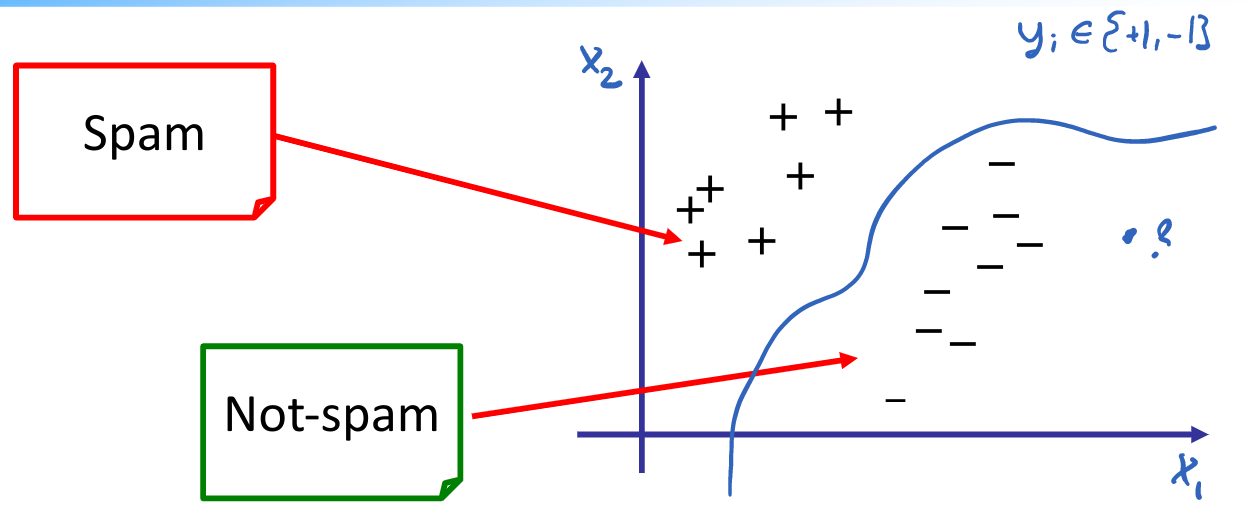
\includegraphics[width=.5\textwidth]{figures/binary_classification.png}
    \caption{Illustration of binary classification}
    \label{binary_classification}
\end{figure}
Given a dataset $D=\left\{(x_1, y_1), \ldots(x_n, y_n)\right\}$, we have:
\begin{equation*}
    y\approx h_{\mathbf{w}}(x)= \text{sign}(w^Tx)
\end{equation*}
Linear classification works well in high-dimensional settings when using the right features; prediction is typically very efficient despite linear classification seeming very restrictive at first.

\subsection{Finding linear separators}

Writing the search for a classifier can be seen as an optimization problem:
we seek the set of weights $\mathbf{w}$ that minimizes the number of mistakes, i.e.:
\begin{align*}
    \hat{\mathbf{w}} &= \arg\min_{\mathbf{w}\in\mathbb{R}}\sum_{i=1}^{n}[y_i\neq \text{sign}(w^Tx_i)]\\
    =\begin{cases}
        1\text{ if } y_i\neq \text{sign}(w^Tx_i)\\
        0\text{ otherwise.}
    \end{cases}
\end{align*}

The goal is then to optimize the following function:
\begin{align*}
    \hat{\mathbf{w}} &= \arg\min_{\mathbf{w}\in\mathbb{R}}\frac{1}{n}\sum_{i=1}^{n}[y_i\neq \text{sign}(w^Tx_i)]\\
    &= \frac{1}{n}\sum_{i=1}^{n}\mathcal{l}(w; x_i,y_i)
\end{align*}
Note that this poses as challenge as it is not convex or even differentiable. Therefore we need to replace this loss by a tractable loss function for the sake of optimization/model fitting. When evaluating a model, we then use the original cost/performance function. The function we can use to optimize in this case is the surrogate loss:
\begin{equation*}
    l_P(\mathbf{w}; y_i, x_i) = \max (0, -y_i\mathbf{w}^Tx_i)
\end{equation*}
which is also referred to as the perceptron loss.

The gradient of the perceptron loss function can be computed as follows:
\begin{align*}
    \hat{R(w)}&=\sum_{i=1}^{n}\max (0, -y_iw^Tx_i)\\
    \nabla\hat{R(w)}&=\sum_{i=1}^{n}\nabla_{\mathbf{w}}\max (0, -y_iw^Tx_i)\\
    &=\begin{cases}
        0\text{ if } y_iw^Tx_i\geq 0 \text{ i.e. correctly classified }
        -y_ix_i\text{ otherwise}
    \end{cases}
\end{align*}

So we have the following update rule:
\begin{equation*}
    \mathbf{w}_{t+1} \leftarrow \mathbf{w}w_t+\eta_t\sum_{i:(x_i,y_i) {incorrectly classified by} w}^{x_iy_i}
\end{equation*}

\subsection{Stochastic gradient descent}
Computing the gradient requires summing over all data, which is inefficient for large datasets. Additionally, our initial estimates are likely very wrong and we can get a good unbiased gradient estimate by evaluating the gradient on few points. In the worst case, we can evaluate only one randomly chosen point, which is a procedure called stochastic gradient descent. It consists of the following steps:
\begin{enumerate}
    \item Start at an arbitrary $\mathbf{w}_0\in\mathbb{R}^d$
    \item For $t=1,2,\ldots$ do:
    \begin{itemize}
        \item Pick data point $(\mathbf{x}',y')\in D$ from training set uniformly at random (with replacement), and set:
        \begin{equation*}
            \mathbf{w}_{t+1}=\mathbf{w}_t-\eta_t\nabla\ell(\mathbf{w}_t;\mathbf{x}',y')
        \end{equation*}
    \end{itemize}
\end{enumerate}
Where $\eta_t$ is called the learning rate. Guaranteed to converge under mild conditions, if:
\begin{equation*}
    \sum_{t}\eta_t=\infty \text{ and }\sum_{t}\eta_t^2<\infty
\end{equation*}
for instance $\eta_t=\frac{1}{t}$ and $\eta_t=\min (c, \frac{c'}{t})$.\\
The perceptron algorithm is just stochastic gradient descent on the perceptron loss function $\ell_P$ with learning rate 1.
\begin{theorem}[Perceptron algorithm]
    If the data is linearly separable, the perceptron will obtain a linear separator.
\end{theorem}
The variance of the gradient estimate can be reduced by averaging over the gradients w.r.t. multiple randomly selected points, which are called minibatches. Adaptive learning rates can be additionally applie. There exist various approaches for adaptively tuning the learning rate. Often times, these even use a different learning rate per feature. Examples of adaptive learning rate algorithms include AdaGrad, RMSProp, Adam, ...
\subsection{Hinge loss vs. perceptron loss}
The Hinge loss encourages the margin of the classifier, and is defined as follows:
\begin{equation*}
    \ell_H(\mathbf{w}; \mathbf{x}, y)=\max\left\{0,1-y\mathbf{w}^T\mathbf{x}\right\}
\end{equation*}

\subsection{Support vector machines}

The optimization objective for the support vector machine is defined as minimizing Hinge loss while also adding another regularization term. There are several lines that need to be considered in the max. margin linear classification, which are summarised in figure \ref{planes_svm}

\begin{figure}
    \centering
    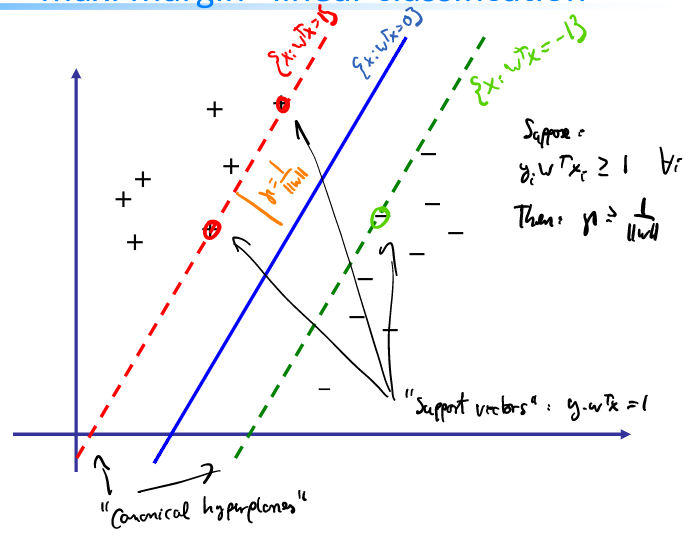
\includegraphics[width=.8\textwidth]{figures/max_margin_decision_boundaries.png}
    \caption{Important elements and their defining equations for support vector machines.}
    \label{planes_svm}
\end{figure}

Support vector machinea re widely used, very effective linear classifiers. They behave almost like a perceptron. The only differences include:
\begin{itemize}
    \item Optimize slightly different, shifted loss (hinge loss)
    \item They regularize the weights
\end{itemize}
It can be optimized using a stochastic gradient descent. A safe choice for the learning rate is:
\begin{equation*}
    \eta_t=\frac{1}{\lambda t}
\end{equation*}

\subsubsection{Stochastic gradient descent for support vector machines}

Let's recall the ojective function:
\begin{equation*}
    \hat{R}(\mathbf{w})=\sum_{i=1}^{n}\ell_{H}(\mathbf{w}_i; x_i,y_i) + \lambda\norm[{\mathbf{w}}_2^2
\end{equation*}
This requires taking care of the regularizer, as follows:
\begin{equation*}
    \hat{R}(\mathbf{w})=\sum_{i=1}^{n}\left(\ell_{H}(\mathbf{w}_i; x_i,y_i) + \frac{\lambda}{n}\norm[{\mathbf{w}}_2^2\right)=f_i(\mathbf{w})
\end{equation*}
So, in order to estimate the gradient $\nabla_{\mathbf{w}}\hat{R}(\mathbf{w})$ which is equivalent to:
\begin{equation*}
    \nabla_{\mathbf{w}}\hat{R}(\mathbf{w})=\sum_{i=1}^{n}\nabla_{\mathbf{w}}f_{i}(\mathbf{w})
\end{equation*}
where:
\begin{equation*}
    \nabla_{\mathbf{w}}f_{i}(\mathbf{w}) = \nabla\ell_{H}(\mathbf{w}+\frac{\lambda}{n}\nabla\norm{\mathbf{w}}_2^2)
\end{equation*}
so the gradient of the regularization term is just $2\mathbf{w}$. For the Hinge loss:
\begin{equation*}
    \nabla\ell_H = \nabla\max(0,1-y_i\mathbf{w}^Tx_i)
    = \begin{cases}
        0\text{ if } y_iw^Tx_i\geq 1\\
        -y_ix_i\text{ otherwise.}
    \end{cases}
\end{equation*}
Therefore the entire update rule for stochastic gradient descent for SVM is:
\begin{equation*}
    \mathbf{w}_{t+1}\leftarrow w_t\left(1-\eta_t\frac{2\lambda}{n}\right)+\left[y_iw^Tx_i\right]
\end{equation*}
The regularization parameter can be picked via cross-validation just like in linear regression. Instead of using the Hinge loss for validation, the target performance metric needs to be used.

\subsection{Key takeaways}
The key takeaways are:
\begin{itemize}
    \item The perceptron is an algorithm for linear classification
    \item It applies SGD on the perceptron loss
    \item Mini-batches exploit parallelism and reduce variance compared to a single sample
    \item The perceptron loss is a convex surrogate function for the 0-1 misclassification loss
    \item It is guaranteed to produce a feasible solution if the data is separable
    \item SGD is much more generally applicable
    \item SVMs are closely related to Perceptron, they use a hinge loss and regularization.
\end{itemize}
Summary so far:
\begin{itemize}
    \item List of represnetations/features: linear hypotheses, nonlinear hypotheses with nonlinear feature transforms.
    \item Model/Objective: loss function (squared loss, 0/1 loss, perceptron loss, Hinge loss) + regularization ($L^2$ norm)
    \item Method: exact solution, gradient descent, mini-batch SGD, convex programming.
    \item Evaluation metric: MSE, accuracy
    \item Model selection: k-fold cross-validation, Monte Carlo CV.
\end{itemize}

\section{Feature selection}
Reasons why we don't want to work with all potentially available features:
\begin{itemize}
    \item interpretability: understand which features are most important
    \item generalizationL simpler models may generalize better
    \item storage computation and cost: if we select the most important features we don't need to store, sum and acquire data for unused features.
\end{itemize}
The naive way to select features is to try all subsets and pick the best features via cross-validation. Greedy feature selection, which is a general purpose approach, consists of greedily add or remove features to maximize cross-validated prediction accuracy and mutual information or other notions of informativeness not discussed here. It can be used for any method, not only linear regression or classifiers.

\subsection{General greedy approach}
Consider the set of features $V=\left\{1,\ldots, d\right\}$. We then define the cost function for scoring subsets S of V. $\hat{L}(S)$ is the cross-validation error using features in S only. More precisely:
\begin{equation*}
    \mathbf{x}_i=[x_{i,1},\ldots,x_{i,d}]\rightarrow\mathbf{x}_{S,i}=[x_{i,j},\ldots,x_{i,j_k}]
\end{equation*}
where $S$ is defined as:
\begin{equation*}
    S=\left\{j,\ldots,j_{k}\right\}, k=|k|
\end{equation*}
We then train the model on $\left\{x_{j,1},y_1,\ldots,x_{j,n},y_n\right\}$, in order to obtain an estimate based on the weights $\hat{\mathbf{w}}_S$ with associated loss $\hat{L}(S)$, which represents the cross-validated performance of the weight estimates $\hat{\mathbf{w}}_S$.

\subsection{Greedy forward selection}
Start with $S=\emptyset$ and $E_0=\infty$, then for $i=1:d$, we find the best element to add, i.e.:
\begin{equation*}
    s_i=\arg\min_{j\in V \setminus S}\hat{L}(S\cup \left\{j\right\})
\end{equation*}
then we compute the error:
\begin{equation*}
    E_i=\hat{L}(S\cup\left\{s_i\right\})
\end{equation*}
if $E_i>E_{i-1}$ break, else set $S\leftarrow \cup\left\{s_i\right\}$

\subsection{Greedy backward selection}
Start with $S=V$ and $E_{d+1}=\infty$, then for $i=d:-1:1$, we find the best element to remove, i.e.:
\begin{equation*}
    s_i=\arg\min_{j\in S}\hat{L}(S\setminus\left\{j\right\})
\end{equation*}
then we compute the error:
\begin{equation*}
    E_i=\hat{L}(S\setminus\left\{s_i\right\})
\end{equation*}
if $E_i>E_{i-1}$ break, else set $S\leftarrow \setminus\left\{s_i\right\}$

\subsection{Advantages and drawbacks of forward vs. backward feature selection}
\begin{table}[htbp]
    \centering
    \begin{tabular}{lll}
        \toprule
        & Forward Feature Selection & Backward Feature Selection\\
        \midrule
        Method Advantages & Faster (if few relevant features) & Can handle ``dependent'' features\\
        \midrule
        Method drawback & Computational cost & Computational cost \\
        \midrule
        & Suboptimal & Suboptimal \\
        \bottomrule
    \end{tabular}
\end{table}

We want a method that simultaneously solves the learning and the feature selection problem via a single optimization step. So far we have only done optimization via sparsity: i.e. explicitely select a subset of features. This is equivalent to constraining $\mathbf{w}$ to be sparse, i.e. contain at most $k$ non-zero entries. Alternatively, we can penalize the number of nonzero entries:
\begin{equation*}
    \hat{\mathbf{w}} = \arg\min_{\mathbf{w}}\sum_{i=1}^{n}(y_i-w^Tx_i)^2+\lambda \norm{w}_0
\end{equation*}
However, this is a difficult combinatorial optimization problem. The key idea then is to replace $\norm{\mathbf{w}}_0$ by a more tractable term.

The idea here is to use $L_1$ as a surrogate for $L_0$, where:
\begin{equation*}
    \norm{w}_1=\sum_{i=1}^{d}|w_i|
\end{equation*}
and we use $\norm{w}_1$ instead of $\norm{w}_0$.

\subsection{Lasso regression}

In ridge regression, we use $\norm{\mathbf{w}}_2^2$ to control the weights. In Lasso, we replace $\norm{\mathbf{w}}_2^2$ by $\norm{\mathbf{w}}_1$, hence leading to the following L1-regularized regression:
\begin{equation*}
    \min_{\mathbf{w}}\lambda\norm{w}_1+\sum_{i=1}^{n}(y_i-\mathbf{w}^Tx_i)^2
\end{equation*}
This alternative penalty encourages coefficients to be exactly 0, which entails an automatic feature selection.

The regularization parameter can be picked using cross-validation.

\subsubsection{L1 regularization in SVM}
The sparsity trick can be applied to SVMs as well:
\begin{equation*}
    \min_{\mathbf{w}}\norm{\mathbf{w}}_1+\sum_{i=1}^{n}\max(0,1-y_i\mathbf{w}^T\mathbf{x}_i)
\end{equation*}
This alternative penalty encourages coefficients to be exactly 0, which ignores thoses features as well, just like in Lasso regression.

\subsection{Solving L1-regularized problems}
The L1-norm is convex. Combined with convex losses, we can obtain convex optimization problems, which include Lasso and L1-SVM. Those problems can, in principle, be solved usng stochastic gradient descent. Convergence is, however, usually slow. and we rarely obtain exact 0 entries. Recent work in convex optimization deals with solving such problems very efficiently using proximal methods.

\begin{table}[htbp]
    \centering
    \begin{tabular}{lll}
        \toprule
        \textbf{Method} & Greedy & L1-regularization \\
        \midrule
        \textbf{Advantages} & \begin{tabular}{@{}c@{}} Applies to any\\ prediction method \end{tabular} & \begin{tabular}{@{}c@{}} Faster (training and\\ feature selection happen\\jointly) \end{tabular} \\
        \midrule
        \textbf{Disadvantages} & \begin{tabular}{@{}c@{}} Slower (need to\\ train many models \end{tabular} & \begin{tabular}{@{}c@{}} Only works for \\ linear model \end{tabular} \\
        \bottomrule
    \end{tabular}
\end{table}

\section{Non-linear prediction with kernels}

\subsection{Revisiting the perceptron/SVM}

There is a fundamental observation to be made here where the optimal hyperplace lies in the span of the data.

\begin{equation*}
    \mathbf{\hat{w}}=\sum_{i=1}^{n}\alpha_iy_i\mathbf{x}_i
\end{equation*}

that means that the output of any of the models discussed so far can be rewritten as a linear combination of the feature inputs that we have seen so far. Proving this losely can be done by stating that SGD starts from 0 and constructs such a representation. A more abstract proof follows from the representer theorem.

\subsection{Reformulating the perceptron}

In order to make the objective function only depend on the inner product of pairs of data point and work implicitely in high-dimensional spaces as long as we can do inner products efficiently, we need to reformula the optimization problem in terms of $\alpha$ instead of $\mathbf{w}$. Therefore, we do the following:

\begin{align*}
    \hat{\mathbf{w}}&\in\arg\min_{\mathbf{w}\in\mathbb{R}^d}\sum_{i=1}^{n}\max(0,-y_i\mathbf{w}^Tx_i)\text{ Note: we make the following anzats: }\hat{\mathbf{w}}=\sum_{j=1}^{n}\alpha_jy_jx_j\\
    &= \sum_{i=1}^{n}\max(0,-y_i(\sum_{j=1}^{n}\alpha_jy_jx_j)^Tx_i)\\
    &= \sum_{i=1}^{n}\max(0,-y_i\sum_{j=1}^{n}\alpha_jy_j(x_j^Tx_i))\\
    \hat{\mathbf{\alpha}}&\in\arg\min_{\mathbf{\alpha}\in\mathbb{R}^n}\sum_{i=1}^{n}\max(0,-c)
\end{align*}

Often, computing $k(\mathbf{x}, \mathbf{x}')$ can be computed much more efficiently than $\phi(\mathbf{x})^T\phi(\mathbf{x}')$. For the polynomial kernel of degree 2, the computational complexity of computing the explicit feature map of the kernel function is in $\mathcal{O}(d^2)$ whereas it is in $\mathcal{O}(d)$ for the kernel computation.

The perceptron can then be reformulated as follows:

\begin{algorithm}[H]
    \SetAlgoLined
    \KwResult{Trained vector $\hat{\alpha}$ used for prediction}
    $\alpha_0\leftarrow 0$\;
    \For{$t=1,\ldots$}{
        Sample $(\mathbf{x}_i, y_i)\sim D$\;
        \uIf{$y_i\sum_{j=1}^{n}\alpha_jy_jk(x_j^Tx_i)>0$}{
            $\alpha_{t+1}\leftarrow\alpha_{t}$\;
        }
        \Else{
            $\alpha_{t+1}\leftarrow\alpha_{t}$\;
            $\alpha_{t+1,i}\leftarrow\alpha_{t+1,i}+\eta_t$\;
        }
    }
    \caption{Kernelized perceptron}
\end{algorithm}

For a new point, we can predict:
\begin{equation*}
    \hat{y}=\text{sign}(\sum_{j=1}^{n}\alpha_jy_jk(\mathbf{x}_j,\mathbf{x}))
\end{equation*}

\subsection{The kernel trick}

Non-linear decision boundaries can be found by using non-linear transformations of the feature vectors followed by linear classification. An important aspect to keep in mind when doing these feature transformation is the dimensionality of the data that is being used. We need, for instance, $\mathcal{O}(d^k)$ dimensions to represent multivariate polynomials of degree $k$ on $d$ features. The challenge then becomes to efficiently implicitely operate in such high-dimensional feature spaces withough ever explicitely computing the transformation.


\begin{definition}[The kernel trick]
    The kernel trick consists in expressing a problem such that it only depends on inter products, which can then be replaced by kernels.
\end{definition}
An example of such a kernel can be applied to the perceptron loss:
\begin{align*}
    \hat{\alpha} &=\arg\min_{\alpha_{1:n}}\frac{1}{n}\sum_{i=1}^{n}\max\left\{0 -\sum_{j=1}^{n}\alpha_jy_iy_jx_i^Tx_j\right\}\\
    \Leftrightarrow \hat{\alpha} &= \arg\min_{\alpha_{1:n}}\frac{1}{n}\sum_{i=1}^{n}\max\left\{0 -\sum_{j=1}^{n}\alpha_jy_iy_jk(\mathbf{x}_j, \mathbf{x}_i)\right\}
\end{align*}

\subsection{The kernelized perceptron}
At training time, the problem can be solved as follows:
\begin{itemize}
    \item Initialize $\alpha_1=\ldots=\alpha_n=0$
    \item For $t=1,2,\ldots$
    \begin{itemize}
        \item Pick data point $(x_i, y_i)$ uniformly at random
        \item Predict:
        \begin{equation*}
            \hat{y} = \text{sign}(\sum_{j=1}^{n}\alpha_jy_jk(\mathbf{x}_j, \mathbf{x}_i))
        \end{equation*}
        \item If $\hat{y}\neq y_i$ set $\alpha\leftarrow \alpha_i+\eta_t$
    \end{itemize}
\end{itemize}
At the time of prediction, for a new point $x$, we predict:
\begin{equation*}
    \hat{y} = \text{sign}(\sum_{j=1}^{n}\alpha_jy_jk(\mathbf{x}_j, \mathbf{x}_i))
\end{equation*}
\subsection{Kernel functions}
\begin{definition}[Kernel functions]
    Given a data space $X$, a kernel is a function $k:X\times X\rightarrow\mathbb{R}$ satisfying the following properties:
    \begin{itemize}
        \item \textbf{Symmetry}: for any pair of vectors $\mathbf{x}, \mathbf{x}'\in X$ it must hold that:
        \begin{equation*}
            k(\mathbf{x}, \mathbf{x}')=k(\mathbf{x}', \mathbf{x})
        \end{equation*}
        \item \textbf{Positive semi-definiteness}: for any $n$, any set $S=\left\{\mathbf{x}_1,\ldots\mathbf{x}_n\right\}\subseteq X$, the kernel (Gram) matrix defined as:
        \begin{equation*}
            K = \begin{bmatrix}
                k(\mathbf{x}_1, \mathbf{x}_1) & \ldots & k(\mathbf{x}_1, \mathbf{x}_n)\\
                \vdots & \ddots & \vdots\\
                k(\mathbf{x}_n, \mathbf{x}_1) & \ldots & k(\mathbf{x}_n, \mathbf{x}_n)\\
            \end{bmatrix}
        \end{equation*}
        must be positive semi-definite.
    \end{itemize}
\end{definition}

A matrix is positive semidefinite iff:
\begin{enumerate}[i]
    \item $\forall x\in\mathbb{R}^n: \mathbf{x}^TM\mathbf{x}\geq 0$
    \item All eigenvalues of $M\geq 0$
\end{enumerate}

Suppose the data space $X=\left\{1,\ldots,n\right\}$ is finite, and we are given a p.s.d. matrix $\mathbf{K}\in\mathbb{R}^{n\times n}$, then we can always construct a feature map:
\begin{equation*}
    \phi:Z\rightarrow \mathbb{R}^n
\end{equation*}
such that $\mathbf{K}_{i,j}=\phi(i)^T\phi(j)$.

\begin{proof}[Proof]
    $\mathbf{K}$ is p.s.d. $\Rightarrow\mathbf{K}=UDU^T$ where $D=\begin{bmatrix}
        \lambda_1 & \ldots & 0\\
        \vdots & \ddots & \vdots\\
        0 & \ldots & \lambda_n
    \end{bmatrix}$ and $\lambda_i\geq 0\forall i$
    We then define a matrix $D=D^{1/2}TD^{1/2}$ where $D^{1/2}
    \begin{bmatrix}
        \sqrt{\lambda_1} & \ldots & 0\\
        \vdots & \ddots & \vdots\\
        0 & \ldots & \sqrt{\lambda_n}
    \end{bmatrix}$ and $\lambda_i\geq 0\forall i
    $. This gives us the following: $\mathbf{K}=UD^{1/2}D^{1/2}U^T=\phi^T\phi$ where $\phi=\left[\phi_1|\ldots|\phi_n\right]$. Now it holds that taking $k(i,j)=\mathbf{K}_{i,j}=\phi_i^T\phi_j$ which means that that $\phi: X\rightarrow \mathbb{R}^n$ and $\phi: i\rightarrow \phi_i$ which is a constructed valid feature map. It shows that for finite data spaces $X$, positive definiteness of the function is also a sufficient condition for it being a valid kernel.
\end{proof}
More generally:
\begin{theorem}[Mercer's theorem]
    Let $X$ be a compact subset of $\mathbb{R}^n$ and $k:X\times X\rightarrow \mathbb{R}^n$ a kernel function. Then one can expand $k$ in a uniformly convergent series of bounded functions $\phi_i$ s.t.
    \begin{equation*}
        k(x, x')=\sum_{i=1}^{\infty}\lambda_i\phi_i(x)\phi_i(x').
    \end{equation*}
\end{theorem}

\subsection{Examples of kernels}
\begin{itemize}
    \item Linear kernel: $k(\mathbf{x},\mathbf{x}')=\mathbf{x}^T\mathbf{x}'$
    \item Polynomial kernel: $k(\mathbf{x},\mathbf{x}')=(\mathbf{x}^T\mathbf{x}'+1)^d$
    \item Gaussian (RBF, squared exponential kernel): $k(\mathbf{x},\mathbf{x}')=\exp(-\norm{\mathbf{x}-\mathbf{x}'}_2^2)/h^2$ where $h^2$ is the bandwidth/length scale parameter.
    \item Laplacian kernel: $k(\mathbf{x},\mathbf{x}')=\exp(-\norm{\mathbf{x}-\mathbf{x}'}_1/h)$
\end{itemize}
\subsection{Examples of non-kernels}
\begin{itemize}
    \item $k(\mathbf{x},\mathbf{x}') = \sin(\mathbf{x})cos(\mathbf{x}')$. It is not symmetric. Take for instance $x=0$ and $x'=\frac{\pi}{2}$
    \item $k(\mathbf{x},\mathbf{x}') = \mathbf{x}^TM\mathbf{x}'\forall \mathbf{x},\mathbf{x}'\in\mathbb{R}^d, M\in\mathbb{R}^{d\times d}$
    \begin{proof}[Proof]
        If $M$ is symmetric: $k(\mathbf{x},\mathbf{x}')=\mathbf{x}^TM^T\mathbf{x}'= \mathbf{x}'^TM^T\mathbf{x}= k(\mathbf{x}', \mathbf{x})$. If $M$ is not symmetric, $k$ in general is not symmetric.
        If $M$ is not positive semi-definite, then the kernel function is not definite, e.g. for the situation where $M=-1$ for the normal dot product.
        If $M$ is positive semi-definite: $M=UD^{\frac{1}{2}}D^{\frac{1}{2}}TU^T=V^TV$ for $V=(UD^{\frac{1}{2}})^T$ then: $k(\mathbf{x}, \mathbf{x}')=\mathbf{x}^TM\mathbf{x}'=\mathbf{x}^TV^TV\mathbf{x}=)(V\mathbf{x})^T(V\mathbf{x}')=\phi (\mathbf{x})^T\phi (\mathbf{x'})$ for $\phi(\mathbf{x})=V\mathbf{x}$
    \end{proof}
\end{itemize}

\subsection{Effect of kernel on function class}

Given a kernel $k$, predictors for kernelized classification have the form:
\begin{equation*}
    \hat{y} = \text{sign}(\sum_{j=1}^{n}\alpha_jy_jk(\mathbf{x}_j,\mathbf{x}))
\end{equation*}

Grafically, it looks like in figure \ref{decision_function_kernelized}.

\begin{figure}[htbp]
    \centering
    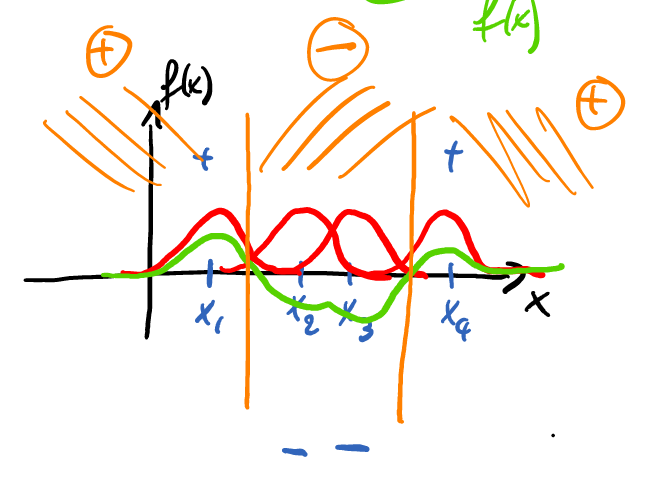
\includegraphics[width=.5\textwidth]{figures/decision_function_kernelized.png}
    \caption{This figure shows that the green line is nothing but a scaled version of the indidiual Gaussian distributions and the associated decision function sign.}
    \label{decision_function_kernelized}
\end{figure}

\subsection{Graphical representations of kernels}

The graphical representation of a sample gaussian and exponential kernel can be found in figures

\begin{figure}[htbp]
    \centering
    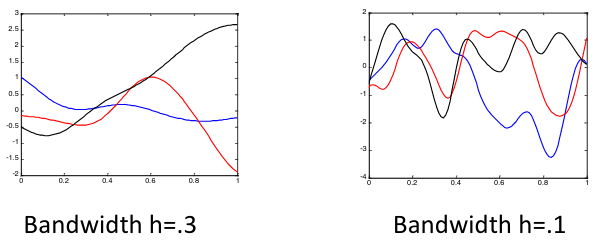
\includegraphics[width=.5\textwidth]{figures/gaussian_kernel.png}
    \caption{Graphical representation of the Gaussian kernel.}
    \label{gaussian_kernel}
\end{figure}

\begin{figure}[htbp]
    \centering
    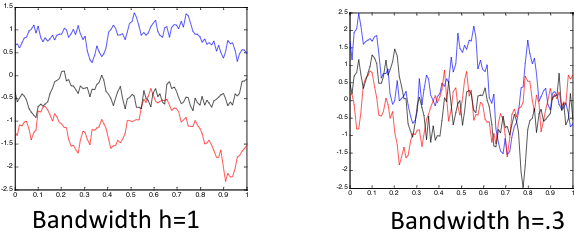
\includegraphics[width=.5\textwidth]{figures/laplacian_kernel.png}
    \caption{Graphical representation of the Laplacian kernel.}
    \label{laplacian_kernel}
\end{figure}

\subsection{Objects where kernels can be used}
The kernels can be defined on a variety of objects:
\begin{itemize}
    \item Sequence kernels
    \item Graph kernels
    \item Diffusion kernels
    \item Kernels on probability distributions
\end{itemize}

Graph kernels can be used for measuring similarity between graphs by comparing random walks on both graphs. They can also be used to measure similarity among nodes in a graph via diffusion kernels not defined here.

\subsection{Kernel engineering}

Suppose we have two kernels:
\begin{equation*}
    k_1:\mathcal{X}\times \mathcal{X}\rightarrow \mathbb{R}\qquad k_2:\mathcal{X}\times \mathcal{X}\rightarrow \mathbb{R}
\end{equation*}
Then the following functions are valid kernels:
\begin{itemize}
    \item $k(\mathbf{x}, \mathbf{x}')=k_1(\mathbf{x}, \mathbf{x}')+k_2(\mathbf{x}, \mathbf{x}')$
    \item $k(\mathbf{x}, \mathbf{x}')=k_1(\mathbf{x}, \mathbf{x}')k_2(\mathbf{x}, \mathbf{x}')$
    \item $k(\mathbf{x}, \mathbf{x}')=ck_1(\mathbf{x}, \mathbf{x}')$ for $c>0$
    \item $k(\mathbf{x}, \mathbf{x}')=f(k_1(\mathbf{x}, \mathbf{x}'))$ where $f$ is a polynomial with positive coefficients or the exponential function.
\end{itemize}

\subsection{The ANOVA kernel}
\begin{equation*}
    k(\mathbf{x}, \mathbf{x}')=\sum_{j=1}^{d}k_j(x_j, x_j')
\end{equation*}
where:
\begin{equation*}
    \mathbf{x}, \mathbf{x}'\in\mathbb{R}^d\qquad k:\mathbb{R}^d\times\mathbb{R}^d\rightarrow \mathbb{R}\qquad k_j:\mathbb{R}\times\mathbb{R}\rightarrow\mathbb{R}
\end{equation*}
The functions modelled by this kernel can be shown by showing what forms $f(x)$ takes:
\begin{align*}
    f(x) &= \sum_{i=1}^{n}\alpha_i y_i k(x^(i),\mathbf{x})\\
    &= \sum_{i=1}^{n}\alpha_i y_i \sum_{j=1}^{d}k_j(x^(i)_j,\mathbf{x}_j)\\
    &= \sum_{j=1}^{d}\sum_{i=1}^{n}\alpha_i y_i k_j(x^(i)_j,\mathbf{x}_j)\\
    &= \sum_{j=1}^{d}f_j(\mathbf{x}_j)
\end{align*}
which means that the function $f$ decomposes into functions that depend on individual coordinates only, i.e. it is additive decomposition of the function. This property can be useful for high dimensional domains.

\subsection{Modelling pairwise data}

Suppose we have the following two kernels:
\begin{align}
    k((x,z),(x', z')) &= k_x(x,x')\cdot k_z(z,z')\\
    k((x,z),(x', z')) &= k_x(x,x') + k_z(z,z')\\
\end{align}
They can be used to represent the following data:
\begin{figure}[htbp]
    \centering
    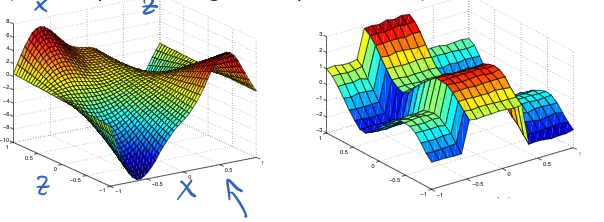
\includegraphics[width=.8\textwidth]{figures/additive_and_multiplicative_effects_of_kernels.png}
    \caption{The left figure can be used to represent a situation where multiplying the kernel could be useful and the right figure can be used to represent a situation where adding the kernel could be useful.}
    \label{additive_and_multiplicative_effects_of_kernels}
\end{figure}

\subsection{Kernels as similarity functions}

Kernels can be used as similarity measures. For instance, consider the Gaussian kernel \\$k(\mathbf{x}, \mathbf{x}')=\exp (-\norm{\mathbf{x}-\mathbf{x}'}^2/h^2)$. If a point $\mathbf{x}$ is close to $\mathbf{x}'$, then the value of $k(\mathbf{x}, \mathbf{x}')\approx 1$, else it is closer to $0$.

\subsection{Comparing k-NN to kernel perceptron}

The prediction for each point in $k$-NN is provided by:
\begin{equation*}
    y=\text{sign}(\sum_{i=1}^{n}y_i\color{blue}[\mathbf{x}\text{ among $k$ nearest neighbors of }\mathbf{x}]\color{black})
\end{equation*}

As we can see, it compares to the loss of the perceptron:

\begin{equation*}
    y=\text{sign}(\sum_{i=1}^{n}y_i\color{blue}\alpha_ik(\mathbf{x}_i,\mathbf{x})\color{black})
\end{equation*}
Note: choose $k$ in $k$-NN using cross-validation.

\begin{table}
    \centering
    \begin{tabular}{lll}
        \toprule
        \textbf{Method} & $k$-NN & Kernelized perceptron\\
        \midrule
        \textbf{Advantages} & No training required & \begin{tabular}{@{}l@{}} Optimized weights can lead to \\ improved performance, can capture \\ global trends with suitable kernels\\ Depends on wrongly classified examples only \end{tabular}\\
        \textbf{Disadvantages} & Depends on all data & Training requires optimisation \\
        \bottomrule
    \end{tabular}
\end{table}

\subsection{Deriving non-parametric models from parametric ones}

Parametric models have a finite set of paramteters. Examples of such models include linear regression, linear perceptron, etc ...
Nonparametric models grow in complexity with the size of the data. They have the potential to be much more expressive but also more computationally complex. Examples of such models include the kernelized perceptron, $k$-NN, etc... Kernels provide a principled way of deriving non-parametrics models from parametric ones.

\subsection{Kernelized SVM}

The SVM optimization step can be kernelized as follows:
\begin{align*}
    \hat{\mathbf{w}}=\arg\min_{\mathbf{w}}\frac{1}{n}\sum_{i=1}^{n}&\max\left\{0,1-y_i\mathbf{w}^T\mathbf{x}_i\right\}+\lambda\norm{\mathbf{w}}_2^2 \qquad \text{ assuming } \mathbf{w}=\sum_{j=1}^{n}\alpha_jy_jx_j\\
    =&\max\left\{0,1-y_i(\sum_{j=1}^{n}\alpha_jy_jx_j)^Tx_i\right\}\\
    =&\max\left\{0,1-y_i\sum_{j=1}^{n}\alpha_jy_j(x_j^Tx_i)\right\}\\
    =&\max\left\{0,1-y_i\sum_{j=1}^{n}\alpha_jy_jk(x_j, x_i)\right\}\\
    =&\max\left\{0,1-y_i\alpha^Tk_i\right\}\\
\end{align*}
where $k_i=\left[y_1k(\mathbf{x}_i, \mathbf{x}_1), \ldots, y_nk(\mathbf{x}_i, \mathbf{x}_n)\right]^T$ and $\alpha = \left[\alpha_1, \ldots, \alpha_n\right]^T$.

The regularizer can be kernelized as follows:
\begin{align*}
    &\lambda\norm{\mathbf{w}}_2^2\\
    =&\lambda\mathbf{w}\mathbf{w}^T=\lambda(\sum_{i=1}^{n}\alpha_iy_ix_i)^T(\sum_{j=1}^{n}\alpha_jy_jx_j)
    =&\lambda\sum_{i=1}^{n}\sum_{j=1}^{n}\alpha_i\alpha_jy_iy_jx_j^Tx_i\\
    =&\lambda\alpha^T D_y\mathbf{K}D_y\alpha
\end{align*}
where $D_y=\begin{bmatrix}
    y_1 & \ldots & 0\\
    \vdots & \ddots & \vdots\\
    0 & \ldots & y_n\\
\end{bmatrix}$ and $\mathbf{K} = \begin{bmatrix}
    k(x_1,x_1) & \ldots & k(x_1,x_n)\\
    \vdots & \ddots & \vdots\\
    k(x_n,x_1) & \ldots & k(x_n,x_n)\\
\end{bmatrix}$

\subsection{Kernelizing linear regression}

Original parametric linear regresion optimization problem is stated as follows:
\begin{equation*}
    \hat{\mathbf{w}}=\arg\min_{\mathbf{w}}\frac{1}{n}\sum_{i=1}^{n}(\mathbf{w}^T\mathbf{x}_i-y_i)^2+\lambda\norm{\mathbf{w}}_2^2
\end{equation*}

We kernelize linear regression in two parts:

\begin{align*}
    =& \sum_{i=1}^{n}(\mathbf{w}^T\mathbf{x}_i-y_i)^2\\
    =& \sum_{i=1}^{n}((\sum_{j=1}^{n}\alpha_jx_jx_i)^T\mathbf{x}_i-y_i)^2\\
    =& \sum_{i=1}^{n}(\sum_{j=1}^{n}\alpha_j(x_j^Tx_i)\mathbf{x}_i-y_i)^2\\
    =& \sum_{i=1}^{n}(\sum_{j=1}^{n}\alpha_j(x_j^Tx_i)\mathbf{x}_i-y_i)^2\\
    =& (\alpha^2k_i-y_i)^2
\end{align*}
and

\begin{align*}
    =& \sum_{i=1}^{n}\sum_{j=1}^{n}\alpha_i\alpha_jx_i^Tx_j\\
    =& \alpha^T\mathbf{K}\alpha
\end{align*}
hence we have:
\begin{align*}
    \hat{\alpha}&=\arg\min_{\alpha\in\mathbb{R^n}}\frac{1}{n}\sum_{i=1}^{n}(\alpha^Tk_i-y_i)^2+\lambda\alpha^T\mathbf{K}\alpha\\
    \hat{\alpha}&=\arg\min_{\alpha\in\mathbb{R^n}}\frac{1}{n}\norm{\alpha^T\mathbf{K}-\mathbf{y}}_2^2+\lambda\alpha^T\mathbf{K}\alpha
\end{align*}
which has a closed-form solution:
\begin{equation*}
    \hat{\alpha}=(\mathbf{K}+n\lambda \mathbf{I})^{-1}\mathbf{y}
\end{equation*}
For prediction, given a data point $\mathbf{x}$, we predict the response $y$ as:
\begin{equation*}
    \hat{y}=\sum_{i=1}^{n}\hat{\alpha_i}k(\mathbf{x_i},\mathbf{x})
\end{equation*}

\subsubsection{Application: semi-parametric regression}

Often, parametric models are too rigid and non-parametric models fail to extrapolate. The solution to this problem is to use additive combination of linear and non-linear kernel function as shown below:

\begin{equation*}
    k(\mathbf{x}, \mathbf{x}') = c_1\exp\left(\norm[]{\mathbf{x} - \mathbf{x}'}_2^2/h^2\right) + c_2\mathbf{x}^T\mathbf{x}'
\end{equation*}

The decision function is then defined as follows:

\begin{align*}
    f(\mathbf{x}) &= \sum_{i=1}^{n}\alpha_i k(\mathbf{x}_i, \mathbf{x})=\sum_{i=1}^{n}\left(\alpha_i(c_i \exp(-\norm[]{\mathbf{x}_i-\mathbf{x}}_2^2/h^2))+c_2\mathbf{x}_i\mathbf{x}'\right)\\
    &= c_1 \sum_{i=1}^{n}\alpha_i k(\mathbf{x}_i,\mathbf{x}) = \sum_{i=1}^{n}\left(\alpha_i(c_1\exp\left(\norm[]{\mathbf{x_i-\mathbf{x}}_2^2/h^2}\right))+c_2\mathbf{x}_i^T\mathbf{x}'\right)\\
    &= c_1\sum_{i=1}^{n}\alpha_i\exp\left(-\norm{\mathbf{x}_i-\mathbf{x}}_2^2/h^2\right) + \left(c_2\sum_{i=1}^{n}\alpha_ix_i\right)^T\mathbf{x}
    &= f_1(\mathbf{x})+\mathbf{w}^T\mathbf{x}
\end{align*}

The efficiency of this methodology can be seen in the figure \ref{semiparametricregression}.

\begin{figure}[htbp]
    \centering
    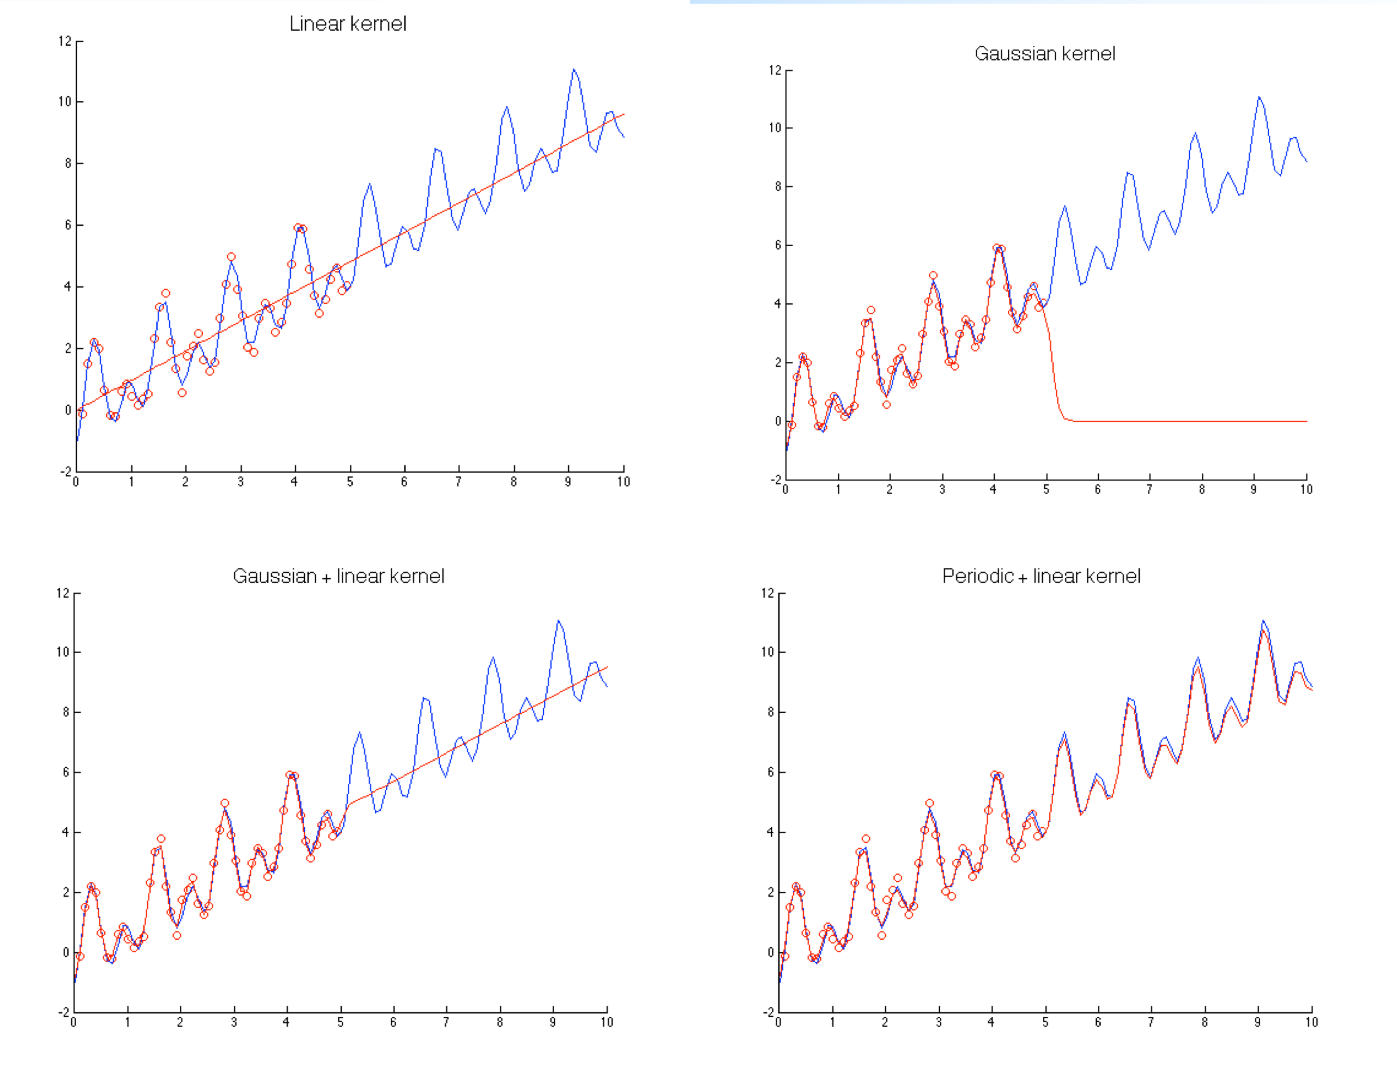
\includegraphics[width=.5\textwidth]{figures/semi-parametric-regression.png}
    \caption{Various learned models overlayed with the function that we wish to learn based on the available data. Clearly, a linear kernel and a periodic parametric model seem to fit best the pattern observed.}
    \label{semiparametricregression}
\end{figure}

This approach can be used to design P450 chimeras, predict protein fitness landscapes, and various other protein engineering applications.

\subsection{Choosing kernels \& risk of overfitting}

Choosing correct kernels is a combination of domain knowledge, brute force or heuristic search using cross-validation. Since kernels map to very high dimensional spaces, it is difficult to see what we hope to be able to learn. Typically the number of parameters is drastically smaller than the number of dimensions. One way of tackling this problem is to set the number of parameters equal to that of the number of datapoints, which in this case would be called non-parametric learning. Another way of tackling this problem is to use regularization, which is built into kernelized linear regression and SVMs but not into the kernelized Perceptron. Recall the formulations of KLR and SVM:
\begin{align*}
    \hat{\alpha} &= \arg\min_{\alpha}\frac{1}{n}\norm[]{\alpha^T\mathbf{K}=\mathbf{y}}_2^2+\lambda\alpha^T\mathbf{K}\alpha\\
    \hat{\alpha} &= \arg\min_{\alpha}\frac{1}{n}\sum_{i=1}^{n}\max\left\{0,1-y_i\alpha^T\mathbf{k}_i\right\} + \lambda\alpha^T\mathbf{D}_{\mathbf{y}}\mathbf{K}\mathbf{D}_\mathbf{y}\alpha
\end{align*}

\section{Class imbalance}

Often data looks very imbalanced, e.g. there are more false negatives than false positives, see figure \ref{imbalanced_data}. Sources of imbalanced data include fraud detection datasets, spam filtering, process monitoring, medical diagnosis, feedback in recommender systems. The main issues related with imbalanced data include \textit{performance metrics}, where the performance assessment of the model is not a good metric. It may be good to prefer certain mistakes over others, i.e. we trade false positives for false negatives. The minority class instance contribute little to the empirical risk. It therefore may be ignored during optimization. There are two solutions to the problem of imbalanced datasets:
\begin{itemize}
    \item \textbf{Subsampling}: this entails removing examples from the majority class (e.g. uniformly at random) such that the resulting dataset is balanced.
    \item \textbf{Upsampling}: this entails repeating data points from the minority class, possibly with small random perturbation to obtain a balanced data set.
    \item It's also a possibility to use cost-sensitive classification methods to deal with these issues.
\end{itemize}

Illustrations of these two approaches are shown in figure \ref{up_and_downsampling}.

\begin{figure}
    \centering
    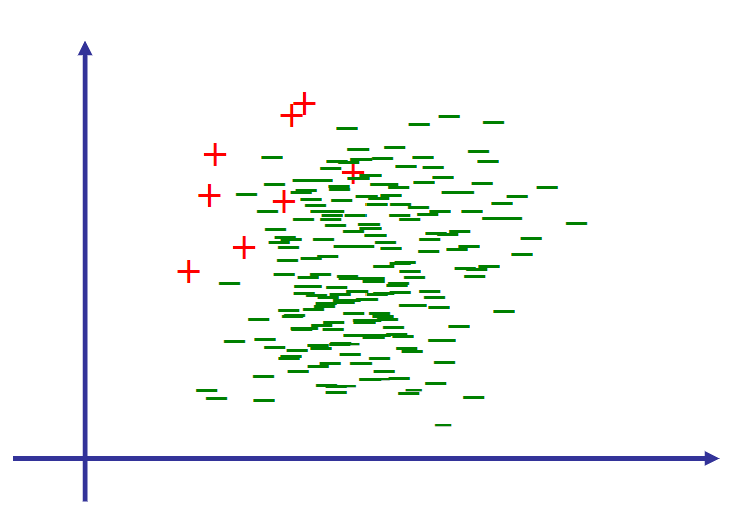
\includegraphics[width=.5\textwidth]{figures/imbalanced_data.png}
    \caption{Example of a dataset with imbalanced data.}
    \label{imbalanced_data}
\end{figure}

\begin{figure}
    \centering
    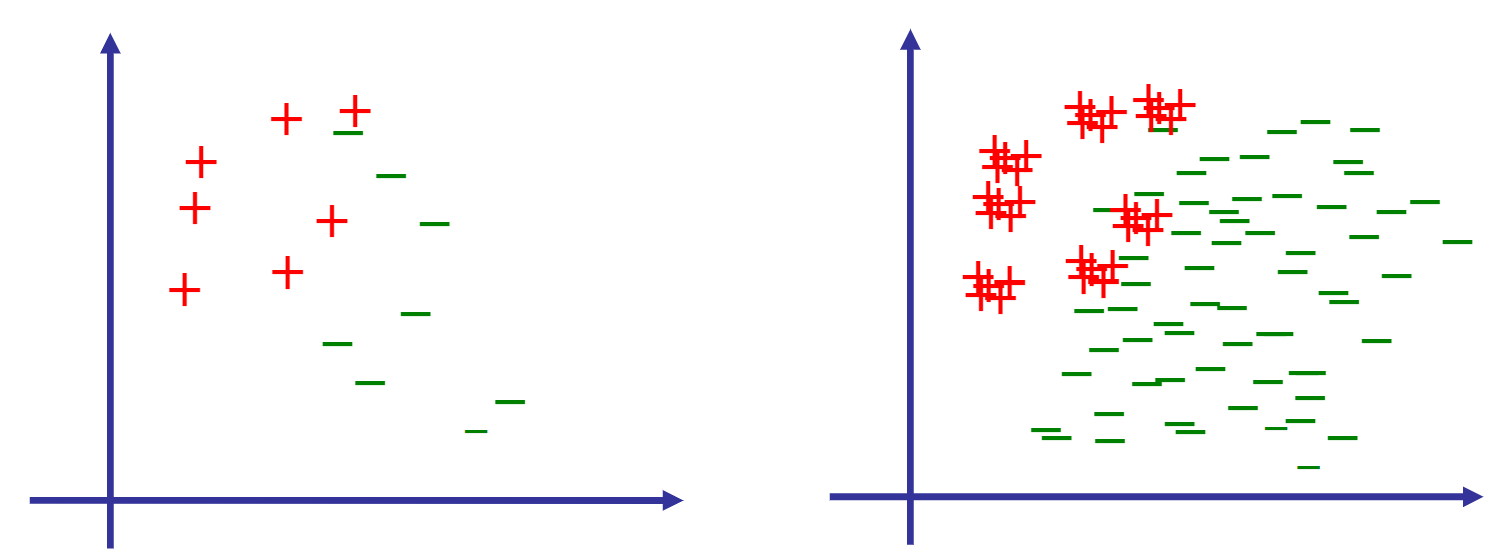
\includegraphics[width=.5\textwidth]{figures/up_and_down_sampling.png}
    \caption{Illustration of subsampling (left) and upsampling (right).}
    \label{up_and_downsampling}
\end{figure}

\subsection{Cost-sensitive classification}

This entails modifying the perceptron/SVM to take class balance into account. The only different is in the cost function, where we add a class coefficient in front of the loss function:
\begin{equation*}
    \ell_{CS}(\mathbf{w};\mathbf{x},y)=\color{blue}c_y\color{black}\ell(\mathbf{w};\mathbf{x},y)
\end{equation*}
For the perceptron, this becomes
\begin{equation*}
    \ell_{CS}(\mathbf{w};\mathbf{x},y)=\color{blue}c_y\color{black}\max(0,-y\mathbf{w}^T\mathbf{x})
\end{equation*}
For the SVM, this becomes
\begin{equation*}
    \ell_{CS}(\mathbf{w};\mathbf{x},y)=\color{blue}c_y\color{black}\max(0,1-y\mathbf{w}^T\mathbf{x})
\end{equation*}
where, in all cases, $c_+, c_->0$ control the tradeoff to be made.

An illustration of the adapted cost function can be seen in figure \ref{perceptron-class-sensitive-loss}.

\begin{figure}
    \centering
    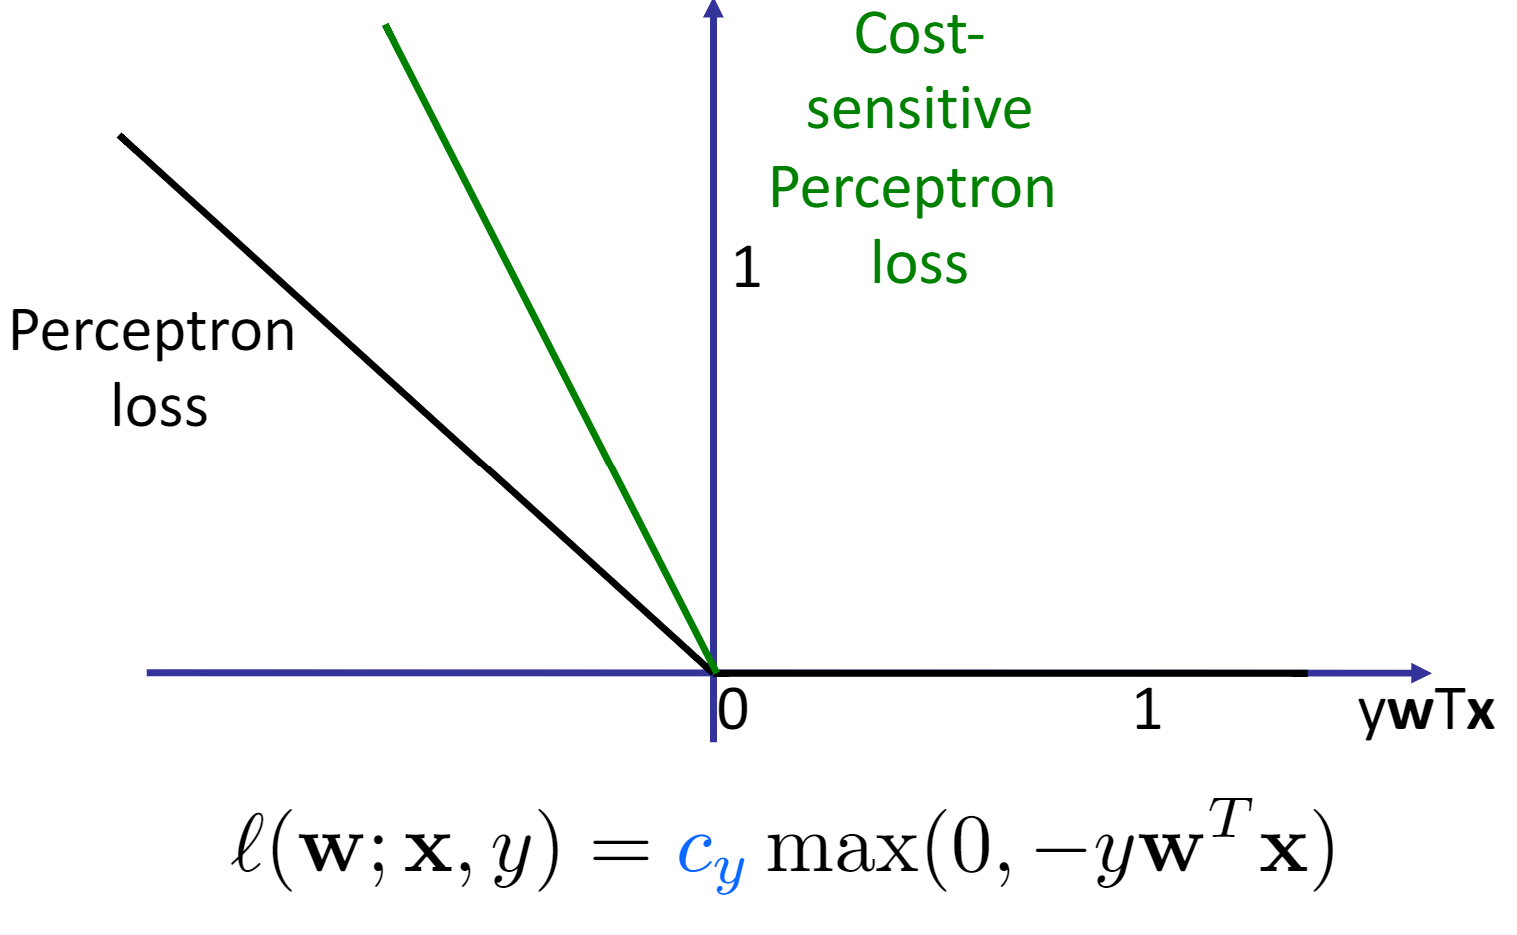
\includegraphics[width=.5\textwidth]{figures/perceptron-class-sensitive-loss.png}
    \caption{Perceptron loss}
    \label{perceptron-class-sensitive-loss}
\end{figure}

\subsection{Avoiding redundancy}

Given that the empirical loss, given by:
\begin{align*}
    \hat{R}(\mathbf{w};c_+,c_-) &= \frac{1}{n}\sum_{i_{y_i=1}}c_+\ell(\mathbf{w};x_i,y_i)+\frac{1}{n}\sum_{i_{y_i=1}}c_-\ell(\mathbf{w};x_i,y_i)\\
    \forall\alpha>0:\hat{R}(\mathbf{w};\alpha c_+, \alpha c_-) &=\alpha\hat{R}(\mathbf{w};c_+,c_-)\\
    \Rightarrow \arg\min_{\mathbf{w}}\hat{R}(\mathbf{w};\alpha c_+, \alpha c_-)&=\arg\min_{\mathbf{w}}\alpha \hat{R}(\mathbf{w}; c_+, c_-)=\arg\min_{\mathbf{w}}\alpha \hat{R}(\mathbf{w}; \frac{c_+}{c_-}, 1)\\
    \Rightarrow \text{w.l.o.g.: } \alpha&=\frac{1}{c_{-}}.
\end{align*}

Which basically means that the tradeoff to make for imbalanced datasets can be determined by one parameter.

\subsection{Metrics for imbalanced datasets}

A generally inappropriate metric for imbalanced datasets is accuracy, defined as
\begin{equation*}
    \text{Accuracy} = \frac{TP+TN}{TP+TN+FP+FN}=\frac{TP+TN}{N}
\end{equation*}
Other, more suitable metrics include:
\begin{equation*}
    \text{Precision}=\frac{TP}{TP+FP}=\frac{TP}{P+}
\end{equation*}
\begin{equation*}
    \text{Recall}=\text{True positive rate (TPR)}=\frac{TP}{TP+FN}=\frac{TP}{N+}
\end{equation*}
\begin{equation*}
    \text{F1 score}=\frac{2TP}{2TP+FN+FP}=\frac{2}{\frac{1}{\text{Prec}}+\frac{1}{\text{Rec}}}
\end{equation*}
\begin{equation*}
    \text{False positive rate (FPR)} = \frac{FP}{TN+FP}
\end{equation*}
An interesting observation to make is that given the probability $p$ of observing a positive sample, we have:
\begin{align*}
    \mathbb{E}[\text{TPR}]&=\frac{\mathbb{E}[\text{TP}]}{n_+}=\frac{p\cdot n_+}{n_+}=p\\
    \mathbb{E}[\text{TPR}]&=\frac{\mathbb{E}[\text{TP}]}{n_-}=\frac{p\cdot n_-}{n_-}=p
\end{align*}

The receiver operator characteristic (ROC) curve (see figure \ref{roc-curve}) can also be used to make an assessment of a classifier.

\begin{figure}
    \centering
    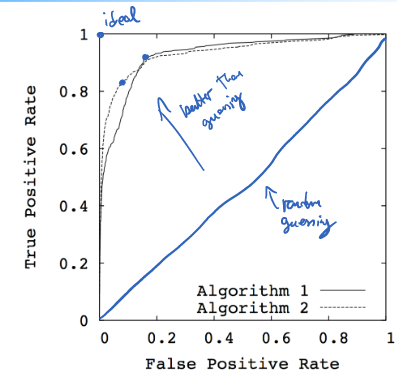
\includegraphics[width=.5\textwidth]{figures/roc_curve.png}
    \caption{}
    \label{roc-curve}
\end{figure}

Note that a performance measure associated to the precision recall curve is the area under the curve. A random classifier has an AUC of 0.5 and an ideal classifier has an AUC of 1.s

It is also important that the confusion matrix itself is also often used to evaluate the performance of a binary or even multi-class classifier.

\begin{table}
    \centering
    \renewcommand\arraystretch{1.5}
    \setlength\tabcolsep{0pt}
    \begin{tabular}{c >{\bfseries}r @{\hspace{0.7em}}c @{\hspace{0.4em}}c @{\hspace{0.7em}}l}
      \multirow{10}{*}{\parbox{1.1cm}{\bfseries\raggedleft actual\\ value}} &
        & \multicolumn{2}{c}{\bfseries Prediction outcome} & \\
      & & \bfseries p & \bfseries n & \bfseries total \\
      & p$'$ & \MyBox{True}{Positive} & \MyBox{False}{Negative} & P$'$ \\[2.4em]
      & n$'$ & \MyBox{False}{Positive} & \MyBox{True}{Negative} & N$'$ \\
      & total & P & N &
    \end{tabular}
\end{table}

\subsection{Obtaining the optimal tradeoff}

Two ways of obtaining a good tradeoff is to either use a cost sensitive classifier and vary the tradeoff parameter. The second option is to find a single classifier and vary the classification threshold $\tau$ in the following formula:
\begin{equation*}
    y=\text{sign}(\mathbf{w}^T\mathbf{x}-\tau)
\end{equation*}

The optimal value for the threshold can be determined using the precision-recall curve \ref{precision-recall-curve}.

\begin{figure}
    \centering
    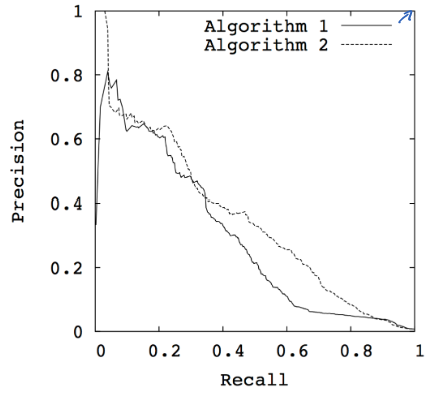
\includegraphics[width=.5\textwidth]{figures/precision_recall_curve.png}
    \caption{An example of a precision-recall curve.}
    \label{precision-recall-curve}
\end{figure}

An interesting note to make in terms of the relationship between the ROC curve and the precision recall curve is captured in the following theorem:

\begin{theorem}
    Algorithm 1 dominates Algorithm 2 in terms of ROC curve $\Leftrightarrow$ Algorithm 1 dominates Algorithm 2 in terms of precision recall curve.
\end{theorem}

\section{Multiclass problems}

A multiclass problem is defined as follows. Given a dataset $\mathcal{D}={(\mathbf{x}_1, y_1),\ldots, (\mathbf{x}_n, y_n)}$ for $y_i\in{1,\ldots, c}$, we want a function $f:\mathcal{X}\rightarrow \mathcal{Y}$ where $y_i\in\mathcal{Y}={1,\ldots,c}$ and $\mathbf{x}_i\in\mathcal{X}\subseteq\mathbb{R}^d$, as illustrated in figure \ref{multiclass-problem}.

\begin{figure}
    \centering
    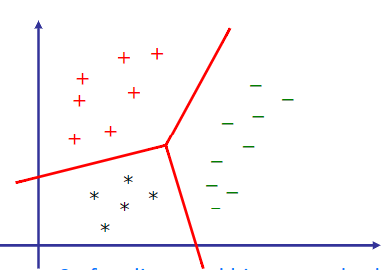
\includegraphics[width=.5\textwidth]{figures/multiclass-problem.png}
    \caption{Illustration of a multiclass problem.}
    \label{multiclass-problem}
\end{figure}

\subsection{One-vs-all}

One approach to solve the problem is to solve $c$ binary classifiers, i.e. one for each class, where all positive samples are from class i and all negative samples represent all other points. We then classify using the classifier with the largest confidence. In other words, we fit $f^{(i)}:\mathcal{X}\rightarrow\mathbb{R}$ and $f^{(i)}(x)=\mathbf{w}^{(i)T}\mathbf{x}$ and we predict $\hat{y}=\arg\max_{i}f^{(i)}(\mathbf{x})=\arg\max_{i}\mathbf{w}^{(i)T}\mathbf{x}$.

\subsubsection{Confidence in a classification}

The confidence in a classification decision can be visualized as in figure \ref{confidence-in-classification}. For $\alpha>0$, we have
\begin{equation*}
    \text{sign}((\alpha\mathbf{w})^T\mathbf{x})=\text{sign}(\mathbf{w}^T\mathbf{x})
\end{equation*}

Thus although $\alpha\mathbf{w}$ and $\mathbf{w}$ implement the same decision boundary, they have a different confidence level. There are two solutions to this problem:
\begin{enumerate}
    \item $\mathbf{w}\leftarrow \frac{\mathbf{w}}{\norm{\mathbf{w}}_2}$, i.e. this is normalized to unit length.
    \item In practice, when using regularization, the magnitude of $\norm[]{\mathbf{w}}_2$ is kept under control.
\end{enumerate}

\begin{figure}
    \centering
    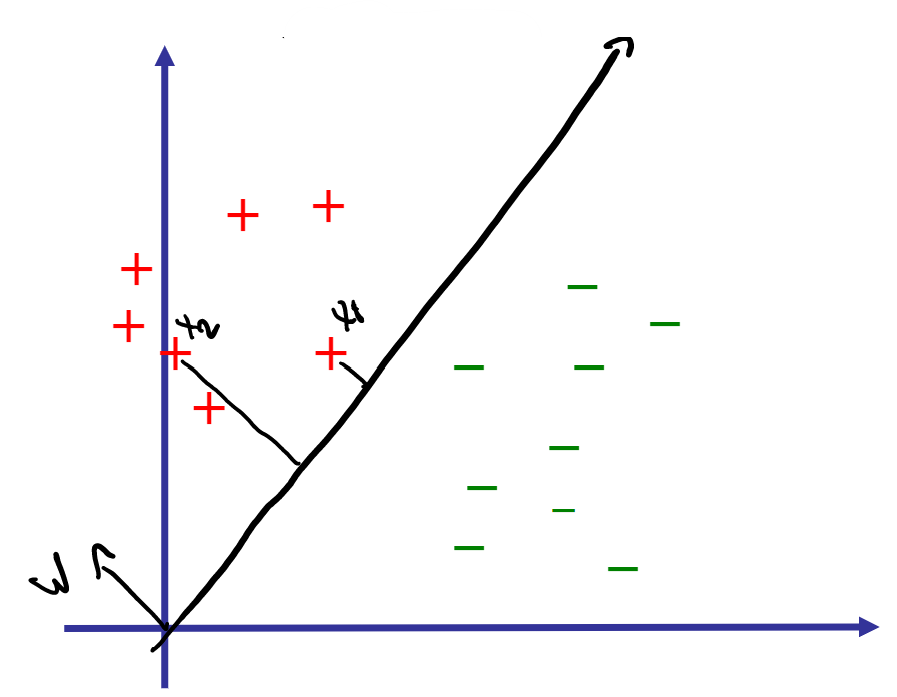
\includegraphics[width=.5\textwidth]{figures/confidence-in-classification.png}
    \caption{Illustration of the confidence in classification. We see that $\mathbf{w}^T\mathbf{x}_2>\mathbf{w}^T\mathbf{x}_1$ so that means that the label + is given with more confidence to $\mathbf{x}_2$ than for $\mathbf{x}_1$}
    \label{confidence-in-classification}
\end{figure}

The decision boundary of the one-vs-all decision can be represented as in figure \ref{ova-decision-boundary}.

\begin{figure}
    \centering
    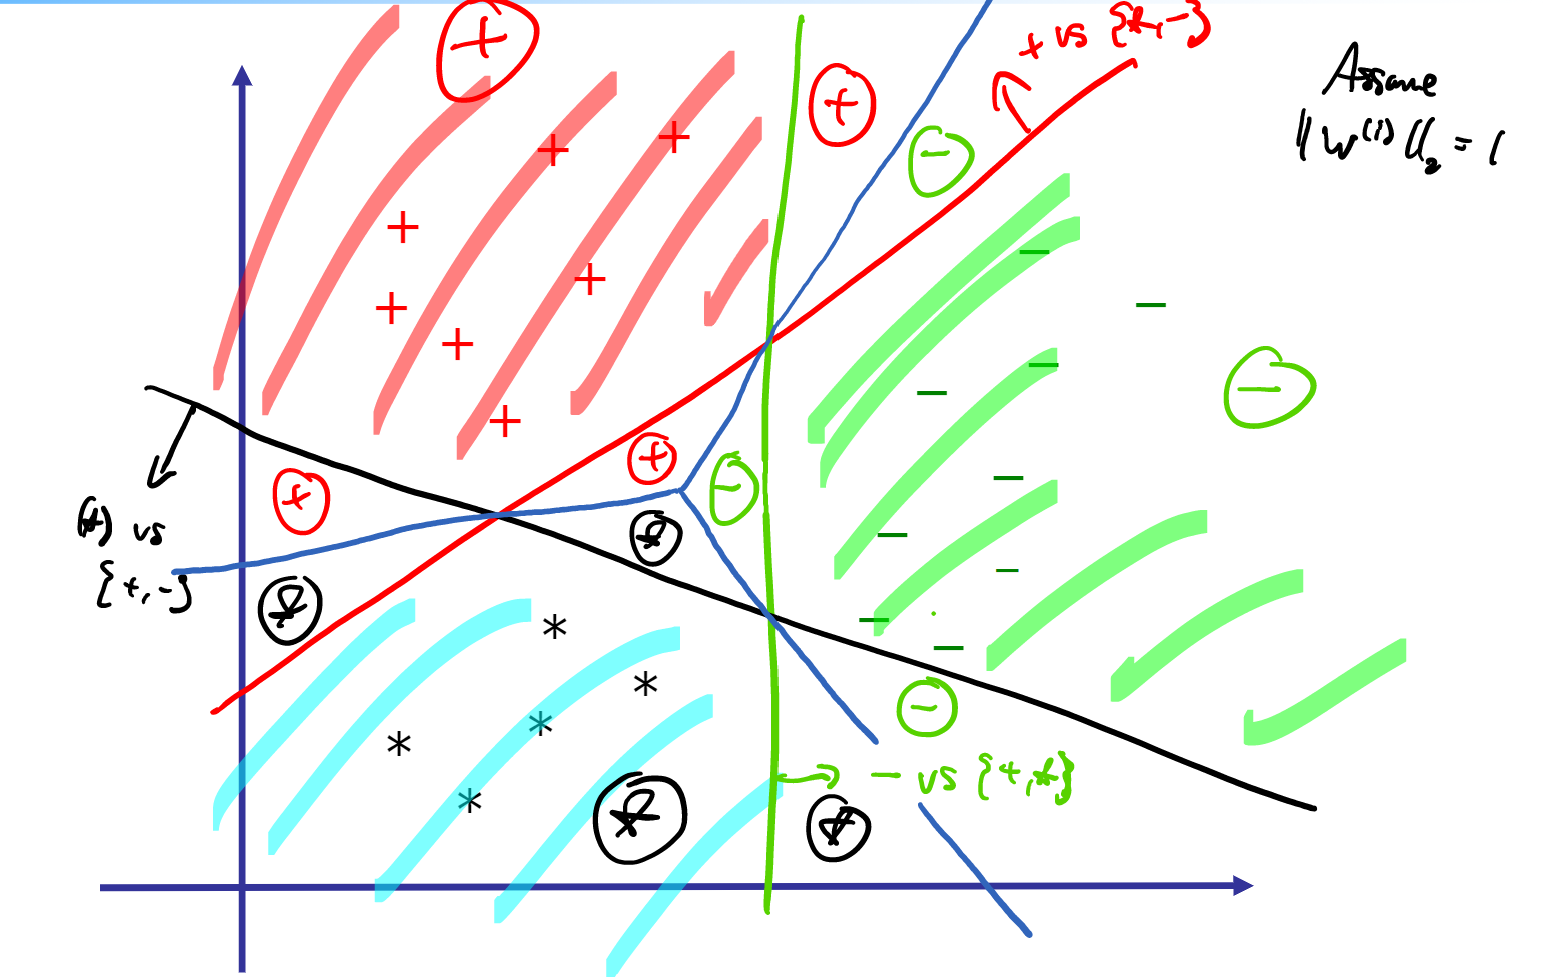
\includegraphics[width=.5\textwidth]{figures/ova-decision-boundary.png}
    \caption{One-vs-all decision boundary.}
    \label{ova-decision-boundary}
\end{figure}

\subsubsection{Challenges}
There are several challenges associated with the one-vs-all technique:
\begin{itemize}
    \item It only works if classifiers produce confidence scores on the same scale.
    \item Individual binary classifier see imbalanced data, even if the whole data set is balanced.
    \item One class might not be linearly separable from all other classes.
\end{itemize}

\subsection{One-vs-one}

The idea is to train $c(c-1)/2$ binary classifiers, one for each pair of classes $(i,j)$. Positive examples contain all points from class $i$ and negative examples contain all points from class $j$. Then, we apply a voting scheme, i.e. the class with the highest number of positive prediction wins. A graphical representation of the one-vs-one classification is shown in figure \ref{one-vs-one}.

\begin{figure}
    \centering
    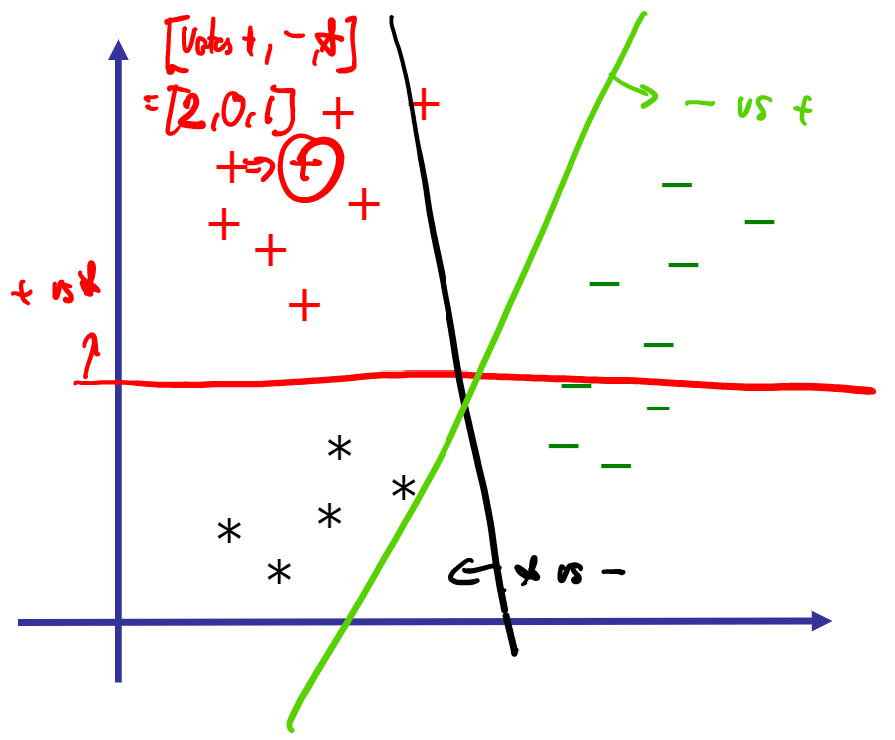
\includegraphics[width=.5\textwidth]{figures/one-vs-one.png}
    \caption{Illustration of the one-vs-one classification technique. Here, we see that each decision boundary is fit for each pair of classes ($i,j$).}
    \label{one-vs-one}
\end{figure}

\begin{table}
    \centering
    \begin{tabular}{lll}
        \toprule
        \textbf{Method} & \textit{One-vs-all} & \textit{One-vs-one} \\
        \midrule
        \textbf{Advantages} & Only $c$ classifiers needed (faster!) & No confidence needed\\
        \textbf{Disadvantages} & Requires confidence + leads to class imbalance & Need to train $c(c-1)/2$)\\
        \bottomrule
    \end{tabular}
\end{table}

\subsection{Encodings}

There are other methods to tackle multiclass problems, e.g. using other encodings (error correcting output codes). There are also other explicit multiclass models, such as the multi-class perceptron/svm etc. Some models are naturally multi-class, such as nearest neighbors, generative probabilistic models, etc. However, one should keep in mind that one-vs-all/one-vs-one usually works very well.

A way to reduce the number of classes we need to work with can be reduce by using an encoding. The length of the encoding will then scale with the $log_{2}c$, see table \ref{binary-label-encoding}. Then in principle the multiclassfication problem is phrased as a decoding task of the class label, where each classifier predicts one bit, which in this case we would get away with $\mathcal{O}(\log c)$ classifiers. In this case, ideas from coding theory to do multi-class classification can be used to do multi-class classification.

\begin{table}
    \centering
    \begin{tabular}{cc}
        \toprule
        \textit{Class} & \textit{Encoding} \\
        \midrule
        0 & [0,0,0,0]\\
        1 & [0,0,0,1]\\
        2 & [0,0,1,0]\\
        \vdots & \vdots\\
        $c-1$ & [1,1,1,1]\\
        \bottomrule
    \end{tabular}
    \caption{Table containing the class name and corresponding encoding}
    \label{binary-label-encoding}
\end{table}

\subsection{Multi-class SVMs}

The key idea of multi-class SVMs is to maintain $c$ weight vectors $\mathbf{w}^{1},\ldots,\mathbf{w}^{c}$, one for each class. Then we predict using:
\begin{equation*}
    \hat{y} \leftarrow \arg\max_{i\in{1,\ldots,c}}\mathbf{w}^{(i)T}\mathbf{x}
\end{equation*}
Given each data point $(\mathbf{x},y)$, we want to achieve that:
\begin{align}\label{multiclasssvm}
    \mathbf{w}^{(y)}\mathbf{x}&\geq\mathbf{w}^{(i)}\mathbf{x}+1 \forall i\in\left\{1,\ldots, c\right\}\setminus{y}\\
    \equiv \mathbf{w}^{(y)}\mathbf{x}&\geq\max_{i\in\left\{1,\ldots,c\right\}\setminus\left\{y\right\}}\mathbf{w}^{(i)}\mathbf{x}+1
\end{align}

\subsection{Multi-class Hinge loss}

\begin{equation*}
    \ell_{MC-H}(\mathbf{w}^{1},\ldots, \mathbf{w}^{c};\mathbf{x}, y)=\max(0,1+\max_{j\in\left\{1,\ldots, y-1,y+1, \ldots,c\right\}} \mathbf{w}^{(j)T}\mathbf{x}-\mathbf{w}^{(y)T}\mathbf{x})
\end{equation*}
which is equal to 0 when equation \ref{multiclasssvm} is satisfied.

The gradient of the Hinge loss is then defined as:
\begin{equation*}
    \nabla_{w^{(i)}}\ell_{MC-H}(\mathbf{w}^{(1:c)};\mathbf{x},y) = \begin{cases}
        0 \text{ if equation \ref{multiclasssvm} is satisfied or } i\neq y\land i\neq \arg\max_{j}\mathbf{w}^{(j)T}\mathbf{x}\\
        -\mathbf{x} \text{ if \ref{multiclasssvm} is not satisfied and } i=y\\
        +\mathbf{x} \text{ otherwise.}
    \end{cases}
\end{equation*}

\section{Neural networks}

\subsection{Importance and characteristics of features}

Succes in learning crucially depends on the quality of features. Hand-designing features however requires domain knowledge. However, kernels could be used to engineer features as they provide a rich set of feature maps, they can fit almost any function with infinite data. However, choosing the right kernel can be challenging and the computational complexity grows exponentially with the size of the data. The question then becomes whether or not we can learn good features from the data directly. The overall objective function for neural networks to optimize is the following:
\begin{equation*}
    \mathbf{w}* =\arg\min_{\mathbf{w}}\sum_{i=1}^{n}\ell(y_i;\sum_{j=1}^{m}w_j\phi_j(\mathbf{x}_j))=\arg\min_{\mathbf{w}}\sum_{i=1}^{n}\ell(y_i;f_i)
\end{equation*}
where $\ell(y_i,f_i)$ is usually defined as $\ell(y_i,f_i)=(y_i-f_i)^2$ (squared loss). A key idea then is to parametrize the feature maps, and optimize over the parameters, i.e. our optimization objective is to tune both the parameters and the weights to minimize the loss:
\begin{equation*}
    \mathbf{w}*=\arg\min_{\mathbf{w},\mathbf{\theta}}\sum_{i=1}^{n}\ell(y_i;\sum_{j=1}^{m}w_j\phi(\mathbf{x}_i,\mathbf{\theta}))
\end{equation*}
One possibility of achieving this optimization is to define the following feature map:
\begin{equation*}
    \phi(\mathbf{x},\mathbf{\theta})=\varphi(\mathbf{\theta}^T\mathbf{x})
\end{equation*}
where $\mathbf{\theta}\in\mathbb{R}^d$ and $\phi:\mathbb{R}\rightarrow\mathbb{R}$ is a nonlinear function, called an \textit{activation function}.
An example of such an activation function is the sigmoid and tanh activation functions. The signmoid function is given by:
\begin{equation*}
    \varphi(z)=\frac{1}{1+\exp(-z)}
\end{equation*}
The tanh function is given by:
\begin{equation*}
    \varphi(z)=\tanh(z)=\frac{exp(z)-\exp(-z)}{exp(z)+\exp(-z)}
\end{equation*}
The rectified linear unit is also often used, which is defined as:
\begin{equation*}
    \phi(z)=\max(z,0)
\end{equation*}
The decision function of an artificial neural network is of the form:
\begin{equation*}
    f(\mathbf{x}_i; \mathbf{w}, \mathbf{\theta})=\sum_{j=1}^{m}w_j\varphi(\theta^T_j\mathbf{x})=\sum_{j=1}^{m}w_jv_j
\end{equation*}
More generally, the term artificial neural network refers to nonlinear functions which are nested compositions of variable linear functions composed with fixed nonlinearities.
\subsection{Graphical representation}
A neural network can be represented as shown in figure \ref{graphical-representation-ann}
\begin{figure}
    \centering
        \begin{tikzpicture}[
            init/.style={
            draw,
            circle,
            inner sep=2pt,
            font=\Huge,
            join = by -latex
            },
            squa/.style={
            draw,
            inner sep=2pt,
            font=\Large,
            join = by -latex
            },
            start chain=2,node distance=13mm
            ]
            \node[on chain=2]
            (x2) {$x_2$};
            \node[on chain=2,join=by o-latex]
            {$w_2$};
            \node[on chain=2,init] (sigma)
            {$\displaystyle\Sigma$};
            \node[on chain=2,squa,label=above:{\parbox{2cm}{\centering Activate \\ function}}]
            {$f$};
            \node[on chain=2,label=above:Output,join=by -latex]
            {$y$};
            \begin{scope}[start chain=1]
            \node[on chain=1] at (0,1.5cm)
            (x1) {$x_1$};
            \node[on chain=1,join=by o-latex]
            (w1) {$w_1$};
            \end{scope}
            \begin{scope}[start chain=3]
            \node[on chain=3] at (0,-1.5cm)
            (x3) {$x_3$};
            \node[on chain=3,label=below:Weights,join=by o-latex]
            (w3) {$w_3$};
            \end{scope}
            \node[label=above:\parbox{2cm}{\centering Bias \\ $b$}] at (sigma|-w1) (b) {};

            \draw[-latex] (w1) -- (sigma);
            \draw[-latex] (w3) -- (sigma);
            \draw[o-latex] (b) -- (sigma);

            \draw[decorate,decoration={brace,mirror}] (x1.north west) -- node[left=10pt] {Inputs} (x3.south west);
        \end{tikzpicture}
    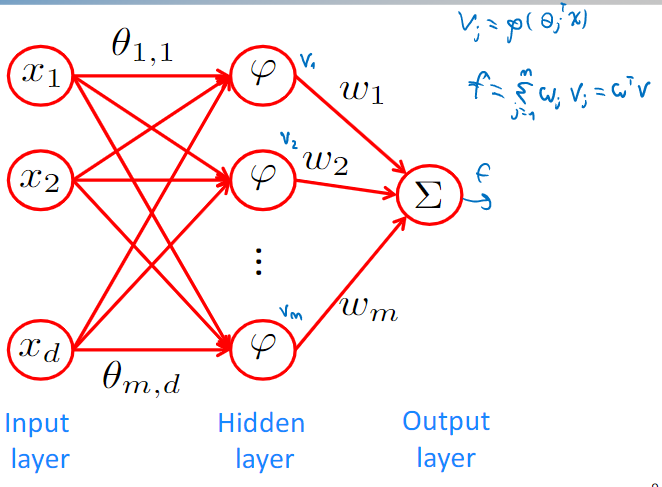
\includegraphics[width=.5\textwidth]{figures/ann-graph-representation.png}
    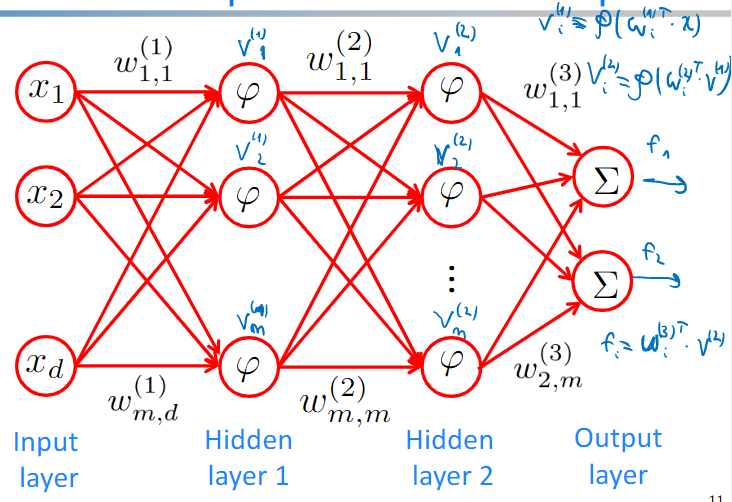
\includegraphics[width=.5\textwidth]{figures/two-layer-ann-representation.png}
    \caption{Graphical representations of an artificial neural network.}
    \label{graphical-representation-ann}
\end{figure}
Note that neural networks can have multiple outputs for multi-class prediction (one output per class or multi-output regression). They can also have more than one hidden layer -- networks with large amounts of neural networks with several hidden layers are called deep neural networks. Indexing in neural networks is done as shown in figure \ref{indexing-ann}.

\begin{figure}
    \centering
    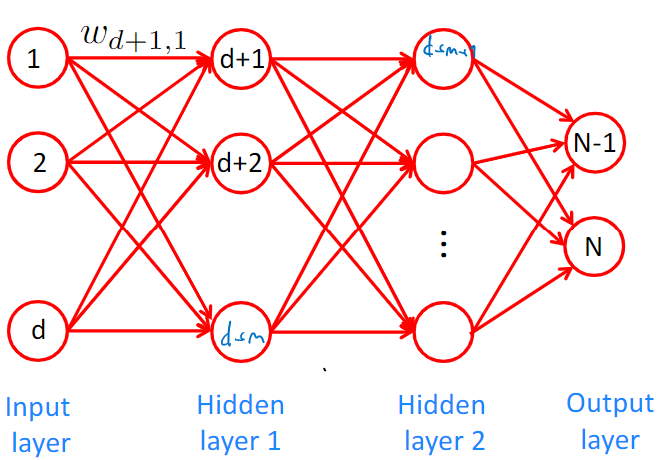
\includegraphics[width=.5\textwidth]{figures/indexing-ann.png}
    \caption{Indexing convention of ANNs}
    \label{indexing-ann}
\end{figure}

\subsection{Making predictions using ANNs}
Suppose we have learned all paramters $w_{i,j}$. Given an input, we now make predictions using forward propagation. The forward propagation procedure is described as follows:
\begin{enumerate}
    \item For each unit $j$ on the input layer, we set its value to $v_j=x_j$.
    \item For each layer $\ell=1:L-1$
    \begin{enumerate}
        \item For each unit $j$ on layer $\ell$ we set its value:
        \begin{equation*}
            v_j=\varphi\left(\sum_{i\in\text{Layer}_{\ell-1}}w_{j,i}v_i\right)
        \end{equation*}
    \end{enumerate}
    \item For each unit $j$ on output layer, set its value:
    \begin{equation*}
        f_j=\sum_{i\in\text{Layer}_{L-1}}^{w_{j,i}v_i}
    \end{equation*}
    \item Predict $y_j=f_j$ for regression, and $y_j=\text{sign}(f_j)$ for regression. For multiclass problems, the prediction is made as $\hat{y}=\arg\max_{j}f_j$.
\end{enumerate}

Another way of writing the forward propagation algorithm is as follows:
\begin{enumerate}
    \item For input layer: $\mathbf{v}^{(0)}=\mathbf{x}$
    \item For each layer $\ell=1:L-1$
    \begin{align*}
        \mathbf{z}^{(\ell)} &= \mathbf{W}^{(\ell)}\mathbf{x}^{(\ell-1)}, \mathbf{z}^{(\ell)}\in\mathbb{R}^{m^{(d)}}\\
        \mathbf{v}^{(\ell)} &=\varphi(\mathbf{z}^{(\ell)})
    \end{align*}
    where $m^{(d)}$ is the number of units in the $\ell$\textsuperscript{th} layer. and $\varphi(\mathbf{z}^{(\ell)}) = [\varphi(\mathbf{z}_1^{(\ell)}), \varphi(\mathbf{z}_2^{(\ell)}),\ldots, \varphi(\mathbf{z}_m^{(\ell)})]$.
    \item For the output layer: $f=\mathbf{W}^{L}\mathbf{v}^{L-1}$
    \item Predict $y=f$ for regression, and $y=\text{sign}(f)$ for regression. For multiclass problems, the prediction is made as $\hat{y}=\arg\max_{i}f_i$.
\end{enumerate}

\subsection{Universal approximation theorem}

Neural networks are powerful modelling tools, because any decision function can be modelled by a sufficiently complex artificial neural networ`k

\begin{theorem}[Universal approximation theorem]
    Let $\sigma$ be any continuous sigmoidal function. Then finite sums of the form:
    \begin{equation*}
        G(x)=\sum_{j=1}^{N}\alpha_j\sigma(y_j^Tx+\sigma_j)
    \end{equation*}
    are dense in $C(I_n)$. In other words, given any $f\in C(I_n)$ and $\epsilon>0$, there is a sum, $G(x)$m of the above form, for which:
    \begin{equation*}
        |G(x)-f(x)|<\epsilon\text{ for all }x\in I_n
    \end{equation*}
\end{theorem}

\subsection{Training the weights of a neural network}

Given a dataset $\mathcal{D} = {(\mathbf{x}_1,y_1),\ldots,(\mathbf{x}_n,y_n)}$, we optimize the weights $\mathbf{W}=(\mathbf{W}^{(1)}, \ldots, \mathbf{W}^{(L)})$ y applying a loss function (e.g. the perceptron loss, the multi-class hinge loss, square loss, etc.) to output:
\begin{equation*}\label{empiricalriskminimisation}
    \ell(\mathbf{W};\mathbf{y}, \mathbf{x})=\ell(\mathbf{y};f(\mathbf{x},\mathbf{x})).
\end{equation*}
Then, we optimize the weights to minimise the loss over $\mathcal{D}$:
\begin{equation*}
    \mathbf{W}*=\arg\min_{\mathbf{W}}\sum_{i=1}^{n}\ell(\mathbf{W};\mathbf{y}_i,\mathbf{x}_i)
\end{equation*}
When predicting multiple outputs at the same time, we usually define the loss as a sum of per-output losses as follows:
\begin{equation*}
    \ell(\mathbf{W};\mathbf{y},\mathbf{x})=\sum_{i=1}^{p}\ell_i(\mathbf{W};y_i,\mathbf{x}).
\end{equation*}
For regression tasks we usually use the squared loss and for classification we use the perceptron or the hinge loss.

Jointy optimizng over all weights for all layers as described in \ref{empiricalriskminimisation} is, in general, a non-convex optimization problem. We can nevertheless try to find a local optimum.

This local optimum can be found, for instance, using stochastic gradient descent, described as follows:
\begin{enumerate}
    \item Initialize the weights $\mathbf{W}$.
    \item For $t=1,2,\ldots$
    \begin{enumerate}
        \item Pick data point $(\mathbf{x}, \mathbf{y})\in\mathcal{D}$ uniformly at random.
        \item Take a step in negative gradient direction:
        \begin{equation*}
            \mathbf{W}\leftarrow \mathbf{W}-\eta_t\nabla_{\mathbf{W}}\ell(\mathbf{W},\mathbf{y},\mathbf{x})
        \end{equation*}
    \end{enumerate}
\end{enumerate}

\subsection{Deep learning}

Generally, deep learning refers to models with nested, layered non-linearities. Common examples of deep neural networks include:
\begin{enumerate}
    \item Classical ANN with multiple layers
    \item Trained via SGD and variants
    \item Some new algorithmic insights (e.g. dropout regularization) and exntensions (Convnets, resnets, RNNs, LSTMs, GRUs,\dots)
\end{enumerate}
Some deep learning success stories include the fact that deep neural networks achieve state of the art performance on some difficult classification tasks such as speech recognition, image recognision, natural language processing and speech translation. A lot of recent work on sequential models such as RNNs, LSTMs, GRUs,\dots have also proven to model data effectively.

Some crucial questions to be answered when training a deep neural network include the following:

\begin{itemize}
    \item How can we compute the gradients?
    \item How should we initialize the weights?
    \item When should we terminate?
    \item How do we choose parameters (number of units/layers/activation functions/learning rate/\dots)?
    \item What about overfitting?
\end{itemize}

\subsection{Computing the gradient}
In order to apply SGD, we need to compute:
\begin{equation*}
    \nabla_{\mathbf{W}}\ell(\mathbf{W};\mathbf{y},\mathbf{x})
\end{equation*}
i.e. for each weight between any two connected units $i$ and $j$, we need to compute:
\begin{equation*}
    \frac{\partial}{\partial w_{i,j}}\ell(\mathbf{W};\mathbf{y},\mathbf{x})
\end{equation*}
In a simple example, we have an ANN with 1 output, 1 hidden and 1 input unit: $\mathbf{W}=[\mathbf{w},\mathbf{w}']$ as shown in figure \ref{simple_ann_differentiation_example}. In this example we have that:
\begin{equation*}
    f(x,\mathbf{W}=w\varphi(w'x)
\end{equation*}
and a dataset containing 1 datapoint containing $\mathcal{D}={(x,y)}$. Then the loss is defined as:
\begin{equation*}
    L(\mathbf{w}',\mathbf{w}) \vcentcolon L = \ell(f,y)=\ell_y(f)
\end{equation*}
Note that $\ell_y(f)$ is computed using forward propagation. Differentiating the loss function w.r.t. the weights gives:
\begin{align*}
    \frac{\partial L}{\partial \mathbf{w}}&=\frac{\partial L}{\partial f}\frac{\partial f}{\partial \mathbf{w}}=\ell_y'(f)\cdot v\\
    \frac{\partial L'}{\partial \mathbf{w}}&=\frac{\partial L}{\partial f}\frac{\partial f}{\partial \mathbf{v}}\frac{\partial \mathbf{v}}{\partial \mathbf{w}'}=\delta\cdot\mathbf{w}\cdot\phi'(z)\cdot \mathbf{x}.
\end{align*}

for instance in the case of the square loss:

\begin{align*}
    \ell_{y}(f)&=(f-y)^2\\
    \Rightarrow l_y'(f)=2(f-y)
\end{align*}

\begin{figure}
    \centering
    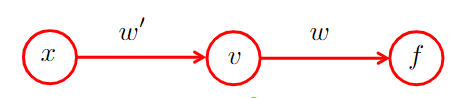
\includegraphics[width=.5\textwidth]{figures/simple_ann_differentiation_example.png}
    \caption{The computation graph of a simple ANN}
    \label{simple_ann_differentiation_example}
\end{figure}

For a slightly more complex example, as depicted in figure \ref{aan-loss-more-complex-example}, the loss is defined as follows:

\begin{equation*}
    L = \sum_{i=1}^{2}\ell_i(\sum_{j}w_{i,j} \varphi(\sum_{k}w'_{j,k} x_k)).
\end{equation*}

The weight vector $\mathbf{W}$ is defined as $\mathbf{W} = [(w_{i,j})_{i,j},(w'_{i,j})_{i,j}]$. The loss is then defined as:

\begin{align*}
    \frac{\partial L}{\partial w_{i,j}}&=\frac{\partial L}{\partial f_{i}}\frac{\partial f_{i}}{\partial w_{i,j}}=\ell'_i(f_i)\cdot v_j\\
\end{align*}

Note that $\ell'_i(f_i)$ and $\cdot v_j$ are computed using forward propagation.

\begin{equation*}
    \frac{\partial L}{\partial w'_{j,k}}=\sum_{i=1}^{2}\frac{\partial L}{\partial f_{i}}\frac{\partial f_i}{\partial v_j}\frac{\partial v_j}{\partial w'_{j,k}}=\sum_{i=1}^{2}\delta_i w_{i,j}\cdot\phi'(z_j)\cdot x_k
\end{equation*}

where $\delta_i=\frac{\partial L}{\partial f_{i}}$ and $\delta '_j=\delta_i w_{i,j}\cdot\phi'(z_j)\cdot x_k$

\begin{figure}
    \centering
    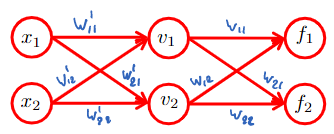
\includegraphics[width=.5\textwidth]{figures/aan-loss-more-complex-example.png}
    \caption{A more complex neural network.}
    \label{aan-loss-more-complex-example}
\end{figure}

\subsubsection{Derivatives of activation functions}

Sigmoid:
\begin{equation*}
    \varphi(z)=\frac{1}{1+\exp(-z)}
\end{equation*}

\begin{equation*}
    \phi'(z)=\frac{-1}{(1+\exp(-z))^2}\cdot e^{-z}\cdot (-1)=\frac{e^{-z}}{1+e^{-z}}\cdot\frac{1}{1+e^{-z}}=\phi(z)(1-\phi(z))
\end{equation*}

The advantage of this function is that it is differentiable everywhere, however $\phi(z)\approx 0$ unless $z=\approx 0$. This leads to a problem that is called a vanishing gradient for deep models.

Rectified linear unit (ReLU):
\begin{equation*}
    \varphi(z)=\max(z,0)
\end{equation*}

\begin{equation*}
    \varphi'(z)=\begin{cases}
        1 \text{ if }z>0\\
        0 \text{ otherwise}
    \end{cases}
\end{equation*}

The disadvantage of this function is that it is not differentiable at 0, but in practice this is not a problem. A huge advantage is $\varphi'(z)=1$ for all $z>0$ which helps with avoiding vanishing gradients.

\subsection{Backpropagation}
The unvectorized version of the backpropagation algorithm is as follows:
\begin{enumerate}
    \item For each unit $j$ on the output layer
    \begin{itemize}
        \item Compute the error signal $\delta_j=\ell_j'(f_j)$
        \item For each unit $i$ on layer $L$, compute $\frac{\partial}{\partial w_{i,j}}=\delta_jv_i$
    \end{itemize}
    \item For each unit $j$ on hidden layer $\ell=L-1:-1:1$
    \begin{itemize}
        \item Compute the error signal: $\delta_j=\phi'(z_j)\sum_{i\in\text{Layer}_{\ell+1}}w_{i,j}\delta_i$
        \item For each unit i on layer $\ell$, compute $\frac{\partial}{\partial w_{i,k}}=\delta_{j}v_i$
    \end{itemize}
\end{enumerate}

The vectorized implementation of the backpropagation algorithm can be phrased as follows:
\begin{enumerate}
    \item For the output layer
    \begin{itemize}
        \item Compute the error $\delta^{L}=\mathbf{\ell'(f)}=[\ell'(f_!),\dots, \ell'(f_p)]$
        \item Gradient: $\nabla_{\mathbf{W}^{(L)}}\ell(\mathbf{W};\mathbf{y},\mathbf{x})=\delta^{(L)}\mathbf{v}^{(L-1)T}$
    \end{itemize}
    \item For each hidden layer $\ell=L-1:-1:1$
    \begin{itemize}
        \item Compute the error $\delta^{(\ell)}=\varphi'(\mathbf{z}^{(\ell)})\odot(\mathbf{W}^{(\ell +1) T}\delta^{(\ell+1)})$:
        \item Compute the gradient: $\nabla_{\mathbf{W}^{(\ell)}}\ell(\mathbf{W};\mathbf{y},\mathbf{x})=\delta^{(\ell)}\mathbf{v}^{(\ell-1)T}$
    \end{itemize}
\end{enumerate}

\subsection{Initializing weights}

Because the optimization problem is non-convex, the initialization of the weights matters, i.e. if we pick innapropriate weights we are more likely to converge towards a suboptimal point in the optimization landscape. Random initialization is often preferred. The rationale of this comes from the propagation of variance. In order to understand why this is the case, assume a node $v_i^{(\ell)}$ with inputs $v_1^{(\ell -1)},\ldots,v_{n_{in}}^{(\ell -1)}$. We know that we carry out the computation $z_i^{(\ell)}=\sum_{j=1}^{n_{in}}w_{ij}v_j^{(\ell-1)}\Rightarrow v_i^{(\ell)}=\phi(z_i^{(\ell)})$ where $\phi(z)=\max(0,z)$.

\subsubsection{Variance propagation}

Now, we assume $\mathbb{E}[x_i]=\mathbb{E}[v_i^{(0)}]=0$ where $v_i^{(0)}$ is the input layer and we also assume that $\text{Var}[x_i]=\text{Var}[v_i^{(0)}]=1$. Let us further assume that the $X_1, \ldots, X_d$ are independent. Additionally, we assume that the weights are draw from a normal distribution, i.e. $w_{ij}\sim\mathcal{N}(0,1)$. Finally, we know that, supposing $X,Y$ are independent with $\mathbb{E}[X]=0$:
\begin{enumerate}[a]
    \item if $\mathbb{E}[Y]=0$, then $\text{Var}(X,Y)=\text{Var}(X)\text{Var}(Y)$
    \item if $\mathbb{E}[Y]\neq 0$, then $\text{Var}(X,Y)=\text{Var}(X)\mathbb{E}[Y^2]$
    \item For ReLU and symmetric $Y$: $\mathbb{E}[\phi(Y)^2]=\frac{1}{2}\text{Var}(Y)$
\end{enumerate}

We then compute:

\begin{align*}
    \mathbb{E}[z_i^{(1)}]&=\mathbb{E}\left[\sum_{j=1}^{n_{in}} w_{i,j}x_j\right]=\sum_{j}\mathbb{E}[w_{ij}]\mathbb{E}[x_j]=0\\
    \text{Var}[z_i^{(1)}]&=\sum_{j}\text{Var}[w_{ij}x_j]\myeq\sum_{j}\text{Var}(w_{ij})\sum_{j}\text{Var}(x_{j})=n\cdot \sigma^{2}\\
    \text{Var}[z_i^{(1)}]&=\sum_{j}\text{Var}\left[w_{ij}v_j^{(\ell - 1)}\right] = \sum_{j}\text{Var}(w_{ij})\mathbb{E}\left[v_j^{(\ell -1)2}\right]=\frac{1}{2}n_{\text{in}}\sigma^2\coloneqq 1\Rightarrow\sigma^2=\frac{2}{n_{\text{in}}}
\end{align*}

This means that in this setting (of course heavily idealized), that the random variables will have the same scale with the same variance across each layer.

\subsubsection{Weight initialization strategies}

The goal of any weight initialization procedure is to keep the variance of weights approximately constant across layers to avoid vanishing and exploding gradients. Usually, random initialization works well, for instance:
\begin{itemize}
    \item Glorot initialization using tanh:
    \begin{align*}
        w_{i,j} &\sim\mathcal{N} (0,1/(n_{in}))\\
        w_{i,j} &\sim\mathcal{N} (0,1/(n_{in}+n_{out}))\\
    \end{align*}
    \item He (ReLU):
    \begin{equation*}
        w_{i,j}\sim\mathcal{N}(0,2/n_{in})
    \end{equation*}
\end{itemize}

The effect of improper initialization strategies is that the weights do not converge over time, as shown in figure \ref{weight-init-he-xavier}.

\begin{figure}
    \centering
    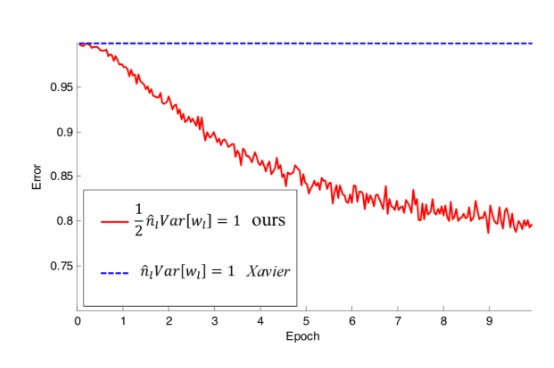
\includegraphics[]{figures/weight-init-he-xavier.png}
    \caption{Weight initialization procedure and effect on training}
    \label{weight-init-he-xavier}
\end{figure}

\subsection{Learning rate}

To implement the SGD rule, a learning rate needs to be chosen. Usually, its a good idea to start with a fixed small learing rate, and decrease slowly after some iteration, e.g.:
\begin{equation*}
    \eta_t=\min (0.1, 100/t)
\end{equation*}
Often, a piecewise constant learning rate schedules the drop in learning rate, e.g. drop after some number of epochs.

Learning with momentum is a common extension to training with SGD as it can help to escale local minima. The idea behind this approach is to not only move into the direction of the gradient, but also in direction of the last weight update. In this case the weight update looks like this:

\begin{align*}
    a&\leftarrow m\cdot a+\eta_t\nabla\ell(\mathbf{W};\mathbf{y},\mathbf{x})
    \mathbf{W}&\leftarrow\mathbf{W}-a
\end{align*}

This allows getting over flatter surfaces of the optimization function quicker while also avoiding oscillations towards the end of the optimization process as we near the optimal point, see figure \ref{oscillation-momentum}.

\begin{figure}
    \centering
    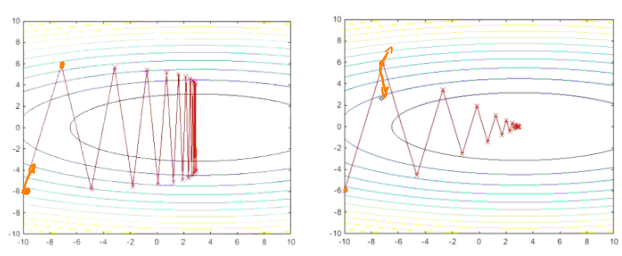
\includegraphics[width=.8\textwidth]{figures/oscillation-momentum.png}
    \caption{Oscillations of the optimization function.}
    \label{oscillation-momentum}
\end{figure}

\subsection{Weight-space symmetries}\label{weight-space-symmetries}

Multiple distinct weights compute the same prediction. I.e. given a network of the topology provided in figure \ref{weight-space-symmetries-fig}, and we define the following variables:
\begin{align*}
    v_i &= \phi(\mathbf{w}_i,x)\\
    f &= w_1'v_1+w_2'v_2\\
    \mathbf{w}=[w_i,w_i']_i&,\bar{\mathbf{w}}=[\bar{w_i},\bar{w_i'}]_i
\end{align*}

Suppose $\bar{\mathbf{w}_2}=\mathbf{{w}}_1$, $\bar{\mathbf{w}_1}=\mathbf{{w}}_2$, $\bar{\mathbf{w}_1'}=\mathbf{{w}}_2'$, $\bar{\mathbf{w}_2'}=\mathbf{{w}}_1'$, we then have:
\begin{equation*}
    f(\mathbf{x};\bar{\mathbf{w}})=f(\mathbf{x};\mathbf{w})
\end{equation*}
which means that multiple local minima can be equivalent in terms of input-output mapping.

For instance, this is valid for the tanh activation function, where $\varphi(z)=-\varphi(-z)$

\begin{figure}
    \centering
    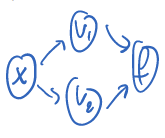
\includegraphics[]{figures/weight-symmetries.png}
    \caption{Network topology used to illustrate weight-space symmetries shown in section \ref{weight-space-symmetries}.}
    \label{weight-space-symmetries-fig}
\end{figure}

\subsection{Avoiding overfitting}

Due to the fact that neural networks have multiple parameters, they have the potential of overfitting the data. There are several countermeasures that can be adopted to mitigate this phenomenon:
\begin{itemize}
    \item Early stopping: it consists in stopping SGD until it converges. This is done by monitoring the prediction performance on a validation set and stop trainign once the validation error starts to increase.
    \item Regularization: add penalty term to keep the weights small.
    \begin{equation*}
        \hat{\mathbf{W}}=\arg\min_{\mathbf{W}}\sum_{i=1}^{n}\ell(\mathbf{W};\mathbf{x}_i,y_i)+\lambda\norm{W}_{F}^2
    \end{equation*}
    \item Dropout: the key idea here is to randomly ignore hidden units during each iteration of SGD with probability $p$. At test time, we then multiply the weights by the probability $p$.
    \item Batch normalization: inputs are shifted and scaled through each layer. Batch normalization is a widely used technique that normalizes inputs to each layer according to mini-batch statistics.
    \begin{itemize}
        \item It reduces internal covariate shift
        \item Enables larger learning rates
        \item It helps with regularization.
    \end{itemize}
\end{itemize}

The algorithm for batch normalization goes as follows:
\begin{enumerate}
    \item \textbf{Input}: values of $x$ over a mini-batch: $\mathcal{B}=\left\{x_1,\ldots,m\right\}$; Parameters to be learned: $\gamma,\beta$
    \item \textbf{Output}: $\left\{y_i=\textnormal{BN}_{\gamma,\beta}(x_i)\right\}$
    \begin{align*}
        \mu_{\mathcal{B}}&\leftarrow\frac{1}{n}\sum_{i=1}^{m}x_i &\text{mini-batch mean}\\
        \sigma_{\mathcal{B}}^2&\leftarrow\frac{1}{n}\sum_{i=1}^{m}(x_i-\mu_{\mathcal{B}})^2&\text{mini-batch variance}\\
        \hat{x_i}&\leftarrow \frac{x_i-\mu_{\mathcal{B}}}{\sqrt{\sigma_{\mathcal{B}}^2+\epsilon}}&\text{normalize}\\
        y_i&\leftarrow \gamma\hat{x}_i+\beta\equiv\text{BN}_{\gamma, \beta}(x_i)&\text{scale and shift}
    \end{align*}
\end{enumerate}
After this procedure, $\phi(\mathbf{w}\mathbf{x})\rightarrow\phi(\mathbf{w}\textnormal{B}_{\gamma,\beta}(\mathbf{x}))$

\subsection{Invariances}
Predictions should be unchanged under some transformations of the data, e.g.
\begin{itemize}
    \item Classification of handwritten digits: the digit can be anywhere on the picture
    \item Speech recognition: the pitch should not matter for classification the speed of the speech should also not matter.
\end{itemize}
A model can be encouraged to learn specific invariances via the following methods:
\begin{itemize}
    \item Augmentation of the training set
    \item Special regularization terms
    \item Invariance built into pre-processing
    \item Implement invariance into structure of ANN, e.g. using convolutional neural networks.
\end{itemize}

\subsection{Convolutional neural networks}
Convolutional neural networks are ANNs for specialized applications, e.g. for image recognition. The hidden layers closest to the input layer shares parameters: each hidden unit only depends on all closeby inputs, e.g. pixels and weights contrained to be identical across all units on the layer. This reduces the number of parameters, and encourages robustness against small amounts of translation. The weights can still be optimized using backpropagation.

The typical CNN architecture that we see is that similar to the one shown in figure \ref{cnn-arch}.

\begin{figure}
    \centering
    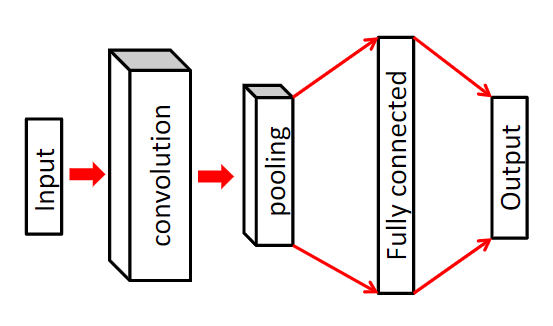
\includegraphics[width=.5\textwidth]{figures/cnn-arch.png}
    \caption{Typical architecture of a CNN}
    \label{cnn-arch}
\end{figure}

Important aspects of CNN have specific terminologies:
\begin{itemize}
    \item Filters/kernels: the size of the filter that passes over an image
    \item Stride: the size of the step taken by the filter at each iteration
    \item Padding: the distance between the border of the image and the first pixel to be processed.
\end{itemize}

Computing the output dimensions of a CNN can be done as follows. Applying $m$ different $f\times f$ filtes to an $n\times n$ image with padding $p$ and stride $s$, we get an output measurement of $\ell=\frac{n+2p-f}{s}+1$. In some applications (e.g. image classification), it can make sense to aggregate several units to decrease the width of the network (and hence the number of parameters).

Pooling layers (equivalent to subsampling) can be added. In some applications, e.g. in image classification, it can make sense to aggregat several units to decrease the width of the network and hence the number of parameters. Usually, one considers either the average or the maximum value of the resulting output of the filter, see figure \ref{max-pooling-layers}.

\begin{figure}
    \centering
    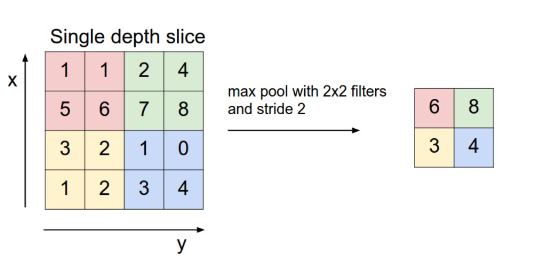
\includegraphics[width=.5\textwidth]{figures/max-pooling-layers.png}
    \caption{Max pooling layers example.}
    \label{max-pooling-layers}
\end{figure}

An example of CNN architecture can be found in figure \ref{cnn-arch}.

\subsection{Computational efficiency}

A key operation for backpropagation training is the dense matrix vector multiplications. These are very suitable on general purpose GPUs and much work on special purpose hardware, for instance TPUs. They have been reponsible for large improvement in computations in recent years.

\subsection{Choice of parameters and architectures}

Several possible activation functions are available. Popular in the past were sigmoid and tanh activations, because they were differentiable. Recently, however, rectified linear units (ReLUs) have been used. Despite being not differentiable, they are very fast to compute and gradients do not vanish, which is important for deep neural networks.

A number of parameters have to be chosen:
\begin{itemize}
    \item The number and width of hidden layers
    \item Use convolution/pooling layers and how many
    \item Skip connections
    \item Type of activation functions
    \item Weight initialization
    \item Learning rate schedule
    \item Regularization method
\end{itemize}

Frameworks for autodifferentiation, e.g. theano, torch and tensorflow. They can use cross-validation to compare models, but training is usually very expensive. They often use single validation (=development) set. Much work is also being done on ML-based experimentaion, i.e. AutoML.

\subsection{ANNs vs. kernels}

When using the tanh activation function, an ANN with a single hidden layer learns functions of the form:
\begin{equation*}
    f(\mathbf{x})=\sum_{i}w_i\tanh\theta^{T}_i\mathbf{x}
\end{equation*}
This is exactly the same type of functions learned with kernels, when using the tanh kernel.
\begin{equation*}
    f(\mathbf{x})=\sum_{i}\alpha_i\tanh\mathbf{x}_i^T\mathbf{x}
\end{equation*}
The difference is that kernels optimize $\alpha$'s only. It is therefore convex. ANNs, however, optimize both $\mathbf{w}'s$ and $\theta_i$, which is a non-convex problem. A more comprehensive comparison of ANNs and kernels is summerized in table \ref{kernels-vs-anns}.

\begin{table}
    \centering
    \begin{tabulary}{\textwidth}{Lp{170pt}p{170pt}}
        \toprule
        \textbf{Method} & \textit{Method} & \textit{ANNs}\\
        \midrule
        \textbf{Advantages} & Convex optimization, no local minima, robust against noise, models grow with the size of the data & Flexible nonlinear models, with fixed parametrization. Multiple layers discover representations at multiple levels of abstraction\\
        \textbf{Disadvantages} & Models grow with the size of data, don't allow multiple layers. & Many free parameters/architectural choices that need to be tuned. Often suffer from very noisy data. \\
    \end{tabulary}
    \label{kernels-vs-anns}
\end{table}

\section{Clustering}

\begin{definition}[Unsupervised learning]
    Unsupervised learning consists of learning a representation of the data without labels, which is typically useful for data analysis, finding patterns and visualization. Most common methods to perform unsupervised learning are clustering and dimensionality reduction.
\end{definition}

\begin{definition}[Clustering]
   Given a set of datapoints, the goal is to group them into clusters such that similar points are in the same cluster and that dissimilar points are in different clusters. Points are typically represented either in (high-dimensional) Euclidean space or with distances specified by a metric or kernel. A related field of clustering is anomaly/outlier detection -- identification of points that don't fit well in any of the clusters.
\end{definition}

Examples of clusterings tasks include:
\begin{itemize}
    \item Documents based on the words they contain
    \item Images based on image features
    \item DNA sequences based on mutation distance
    \item Products based on which customers bought them
    \item Customers based on their purchase history
    \item Web surfers based on their queries/sites they visit.
\end{itemize}

There are several standard approaches to clustering:
\begin{itemize}
    \item \textbf{Hierarchical clustering}: it consists of building a tree (bottom-up or top-down) representing distances among data points. For instance, this includes single-, average-linkage clustering.
    \item \textbf{Partitional approaches}: it consists in defining and optimizing a notion of cost defined over partitions: for instance, this includes spectral clustering, graph-cut based approaches.
    \item \textbf{Model-based approaches}: these methods consist in maintaining cluster models and infer cluster membership, e.g. assign each point to the closest cluster. Examples of model-based approaches include $k$-means clustering, Gaussian mixture models, etc...
\end{itemize}

\subsection{$k$-means clustering}

\subsubsection{Intuition}

The idea behind $k$-means clustering is that every cluster is represented by a single point (named $\mu_j\in\mathbb{R}$) and each point is assigned to the closest center, for instance for cluster 1:
\begin{equation*}
    \left\{\mathbf{x}:1\arg\min_{j}\norm{\mathbf{x}-\mu_j}\right\}
\end{equation*}

This induces a Voronoi partition. See also figure \ref{k-means-clustering-illustration} for an illustration.


\begin{figure}
    \centering
    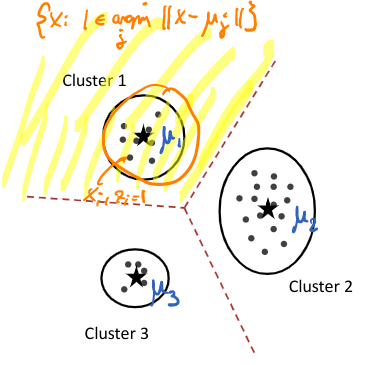
\includegraphics[width=.5\textwidth]{figures/k-means-clustering-illustration.png}
    \caption{$k$-means clustering illustration}
    \label{k-means-clustering-illustration}
\end{figure}

\subsubsection{The problem}

For $k$-means clustering, we assume that the points are in Euclidean space, i.e. $\mathbf{x}\in\mathbb{R}^{d}$. We represent each cluster as a center $\mu\in\mathbb{R}^d$ and each point is assigned to the closest center. The overall goal is to pick centers to minimize the average squared distance:
\begin{equation*}
    \hat{R}(\mu)=\hat{R}(\mu_1, \ldots, \mu_k) = \sum_{i=1}^{n}\min_{j\in\left\{1,\ldots,k\right\}}\norm{\mathbf{x_i}-\mu_j}_2^2
\end{equation*}
and:
\begin{equation*}
    \hat{\mu}=\arg\min_{\mu}\hat{R}(\mu)
\end{equation*}
This is a non-convex optimization problem and is NP-hard in nature, which means that we can't solve this problem optimally in general.

\subsubsection{Lloyd's heuristic}
Lloyd's algorithm consists in:
\begin{itemize}
    \item Initialize the cluster centers $\mu_0=[\mu_1^{(0)},\ldots,\mu_k^{(0)}]$
    \item While the function does not converge:
    \begin{itemize}
        \item Assign each point $\mathbf{x}_i$ to closest center, i.e.:
        \begin{equation*}
            z_i^{t}\leftarrow \arg\min_{j\in\left\{1,\ldots,k\right\}}4\norm{\mathbf{x}_i-\mu_j^{t-1}}.
        \end{equation*}
        \item We then update the center as being the mean of all the points assigned to that center, i.e.:
        \begin{equation*}
            \mu_j^{(t)}\leftarrow\frac{1}{n_j}\sum_{i:z_i^{(t)}=j}\mathbf{x}_i
        \end{equation*}
        where:
        \begin{equation*}
            n_j=\left|\left\{i:z_i^{(t)=j}\right\}\right|.
        \end{equation*}
    \end{itemize}
\end{itemize}

\subsubsection{Properties of $k$-means}

$k$-means is guaranteed to monotonically decrease the average squared distance in each iteration, i.e. $\hat{R}(\mu^{(t)})\geq\hat{R}(\mu^{(t+1)})$.

\begin{proof}[Proof that $k$-means monotonically decreases]
    We know that $\hat{R}(\mu^{(t)})$ is defined by \\
    $\hat{R}(\mu^{(t)})=\sum_{i=1}^{n}\min_{j\in\left\{1,\ldots, k\right\}}\norm{\mathbf{x}_i-\mu_j^{(t)}}_2^2$ at a given timestep $t$. Our objective is to find $\mu_{z_i}$ s.t. $\hat{R}(\mu)=\min_{z}\hat{R}(\mu, z)$ (i.e. the set of cluster center assignments such that the distance is minimized). \\

    We know that $\hat{R}(\mu,z)=\sum_{i=1}^{n}\norm[]{\mathbf{x}_i-\mu_{z_i}}_2^2$. Then, it can be shown that:


    \begin{equation*}
        \hat{R}(\mu^{(t)}, z^{(t)})\geq \hat{R}(\mu^{(t)}, z^{(t+1)})\geq \hat{R}(\mu^{(t+1)}, z^{(t+1)})
    \end{equation*}
    Since $z^{(t+1)}=\arg\min_{\mathbf{z}}\hat{R}(\mu^{(t)}, \mathbf{z})$ we can infer that $\hat{R}(\mu^{(t)}, z^{(t)})\geq \hat{R}(\mu^{(t)}, z^{(t+1)})$ and since $\mu^{(t)}=\arg\min_{\mu}=\hat{R})(\mu, z^{(t+1)})$, which means it converges to a local optimum.
\end{proof}

The complexity per iteration of the algorithm is in $\mathcal{O}(n\cdot k\cdot d)$.

As noted in the proof, the algorithm converges towards a local optimum. A graphical representation of such an event can be seen in figure \ref{local_optimum_k_means}.

\begin{figure}
    \centering
    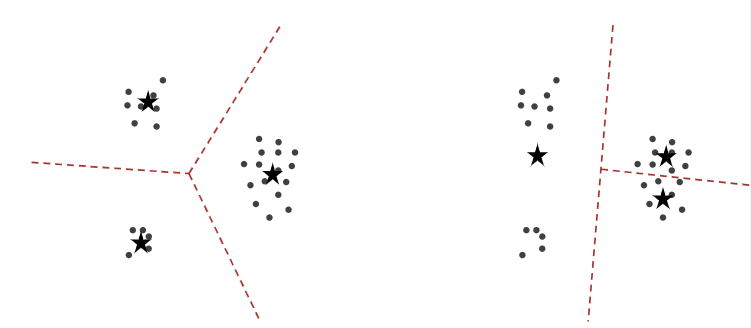
\includegraphics[width=.5\textwidth]{figures/local_optimum_k_means.png}
    \caption{Local optima of a $k$-means algorithmiteration}
    \label{local_optimum_knn}
\end{figure}

\subsubsection{Challenges with $k$-means}

There are multiple challenges when performing $k$-means. Generally, the algorithm only converges to a local optimum, and the performance of the methodology is strongly dependent on the initialization. The number of iterations required can be exponential, even in the place. In practice however the algorithm converges very quickly. Determining the number of clusters $k$ is difficult, and cannot model clusters of arbitrary shape, although kernel Kernel-$k$-means can be used to fix this.

\subsubsection{Initializing $k$-means}
Lloyd's heuristic does not generally converge to the optimal solution. The performance heavily depends on the initialization. Several approaches towards solving the initialization problem are listed below:
\begin{itemize}
    \item Multiple random restarts
    \item Farthest points heuristic, which often works well but is prone to outliers.
    \item Seeding with $k$-means ++.
    \item Other methods exist as well.
\end{itemize}

\subsection{$k$-means ++}
The idea behind $k$-means ++ is to increase the sampling probability of sampling initial points that are likely far away from the center of the cluster.

The algorithm consists of the following steps:
\begin{enumerate}
    \item Start with a random data point as a center, where $i\sim\text{Uniform}(\left\{1,\ldots, n\right\})$ and $\mu_0=x_i$.
    \item Add centers 2 to $k$ randomly, proportionally to the squared distance to the closest selected center, i.e. for $j=2:k$, pick $ij$ with probability $\frac{1}{z}\cdot d(x_{ij};\mu_{1:j-1}^{(0)})$ where $d(x_{ij};\mu_{1:j-1}^{(0)})=\min_{\ell\in\left\{1,\ldots, j-1\right\}}\norm{\mathbf{x}_ij-\mu_{\ell}^{(0)}}_2^2$ and assign: $\mu_j^{(0)}=x_{ij}$
\end{enumerate}

We can show that the expected cost of this procedure is in $\mathcal{O(\log(k))}$ times that of optimal $k$-means solutions: $\mathbb{E}[\hat{R}(\mu^{(0)})]\leq\mathcal{O}(\log k)\min_{\mu}\hat{R}(\mu)$

\subsection{Model selection in clustering}

In general, model selection is very difficult in clustering. There are, however, several approaches that can be adopted. For instance:
\begin{itemize}
    \item heuristic quality measures
    \item regularization (i.e. favor simple models with few parameters by penalizing complex models)
    \item Information theoretic basis (tradeoff between robustness (stability) and informativeness), which can be derived from statistical learning theory.
\end{itemize}

A heuristic for determing $k$ in $k$ means is to use a loss function and plot this value against the number of clusters chosen. Then the optimal choice is made when there is a $k$ such that increasing $k$ leads to neglibible decreases in loss, as see in figure \ref{choice-of-k}

\begin{figure}[]
    \centering
    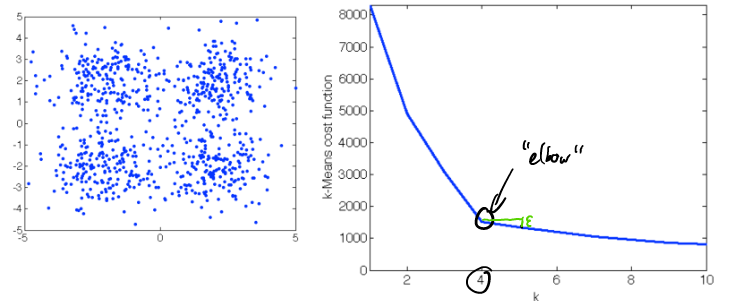
\includegraphics[width=.5\textwidth]{figures/choice-of-k.png}
    \caption{An instance of a choice of $k$, here 4.}
    \label{choice-of-k}
\end{figure}

\subsection{Regularization}

A regularization term can be added to the optimization objective such that more complex models are penalized. For $k$-means, this can be done as follows:

\begin{equation*}
    \min_{k, \mu_{i:k}}\hat{R}(\mu_{i:k})+\lambda\cdot k.
\end{equation*}

Graphically, this is introduces an elbow in the plot of the cost of the loss functions vs. the number of clusters, see figure \ref{regularization_k_means}.

\begin{figure}
    \centering
    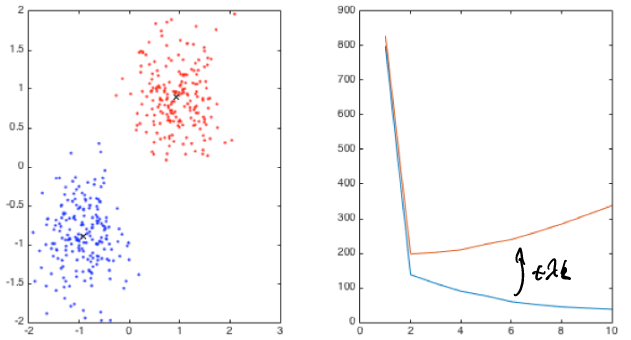
\includegraphics[width=.5\textwidth]{figures/regularization_k_means.png}
    \caption{Illustration of the effect of regularization on the cost function.}
    \label{regularization_k_means}
\end{figure}

Note that the test loss cannot be used to determine the number of clusters, as this loss typically also keeps decreasing.

Challenges with $k$-means which are not a big issue in practice include:
\begin{itemize}
    \item Only a local optimum can be reached in general.
    \item The number of iterations required can be exponential.
\end{itemize}
Challenges with $k$-means which can be fixed via kernel $k$-means, etc.
\begin{itemize}
    \item It is not possible to model clusters of arbitrary shape.
\end{itemize}
A major unsolved practical problem is the choice of number of clusters $k$, which is difficult.

\section{Dimensionality reduction}

The basic challenge is that, given a dataset $\mathcal{D}=\left\{\mathbf{x}_1,\ldots, \mathbf{x}_n\right\}\forall\mathbf{x}_i\in\mathbb{R}^{d}$, we want to obtain an ``embedding'', i.e. a low dimensional representation $\mathbf{z}_1, \ldots, \mathbf{z}_n\in\mathbb{R}^k$ where $k<d$. This serves multiple purpose, including:
\begin{itemize}
    \item visualization for $k=1,2,3$
    \item Regularization (model selection)
    \item Unsupervised feature discovery (i.e. determine features from data)
\end{itemize}

Typical approaches to achieve this problem achieve the following:

\begin{enumerate}
    \item Assume $\mathcal{D}=\left\{\mathbf{x}_1,\ldots, \mathbf{x}_n\right\}\forall\mathbf{x}_i\subseteq\mathbb{R}^{d}$
    \item Obtain a mapping $\mathbf{f}:\mathbb{R}^{d}\rightarrow\mathbb{R}^{k}$ where $k\ll d$.
\end{enumerate}

It is possible to distinguish between the following:
\begin{itemize}
    \item Linear dimension reduction, i.e. $\mathbf{f(x)}=\mathbf{Ax}\forall A\in\mathbb{R}^{k\times d}$
    \item Nonlinear dimension reduction:
    \begin{itemize}
        \item Parametric
        \item Non-parametric
    \end{itemize}
\end{itemize}

A key question in the field then arises: which mappings should we prefer?

\subsection{Linear dimension reduction as compression}

The motivation behind linear dimension reduction is that a low-dimensional representation should allow to compress the original data (accurate reconstruction). For instance, if we set $k=1$, and given a dataset $\mathcal{D}=\left\{\mathbf{x}_1,\ldots, \mathbf{x}_n\right\}\forall\mathbf{x}_i\subseteq\mathbb{R}^{d}$, we want to represent data as points on a line $\mathbf{w}\in\mathbb{R}^d$ with coefficiens $z_1,\ldots, z_n$, i.e. we want $z_i\mathbf{w}\approx\mathbf{x}_i$, assuming $\mu=\frac{1}{n}\sum_{i}\mathbf{x}_i=0$ as shown in figure \ref{linear_dim_reduc}.

\begin{figure}
    \centering
    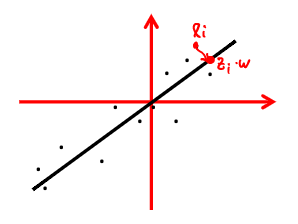
\includegraphics[width=.5\textwidth]{figures/linear-dim-reduc.png}
    \caption{Graphical representation of linear dimension reduction with $k=1$.}
    \label{linear_dim_reduc}
\end{figure}

\subsection{Linear dimension reduction for reconstruction}

Given a dataset $\mathcal{D}=\left\{\mathbf{x}_1,\ldots, \mathbf{x}_n\right\}\forall\mathbf{x}_i\subseteq\mathbb{R}^{d}$, we want $z_i\mathbf{w}\approx\mathbf{x}_i$, e.g. minimizing $\norm{z_i\mathbf{w}=\mathbf{x}_i}_2^2$. To ensure uniqueness, we can normalize $\norm{\mathbf{w}}_2=1$, and then we optimize over $\mathbf{w}, z_1, \ldots, z_n$ jointly:

\begin{equation*}
    (\mathbf{w}*,z_{1:n}*) = \arg\min_{\norm{\mathbf{w}}_2 = 1, \mathbf{z}}\sum_{i=1}^{n}\norm{\mathbf{x}_i-z_i\cdot\mathbf{w}}_2^2 = \hat{R}(\mathbf{w}, z_{1:n})
\end{equation*}

Solving this equation for $\mathbf{z}$ given a vector $\mathbf{w}$ and we get:

\begin{equation*}
    z_i*=\mathbf{w}^T\mathbf{x}_i
\end{equation*}

Thus we effectively solve a regression problem, interpreting $\mathbf{x}$ as features and $z$ as labels. So, we obtain:

\begin{align*}
    \mathbf{w}*&=\arg\min_{\norm{w}_2=1}\sum_{i=1}^{n}\norm{\mathbf{w}\mathbf{w}^T\mathbf{x}_i-\mathbf{x}_i}_2^2\\
    &= \sum_{i=1}^{n}\norm{x_i}_2^2-\sum_{i=1}^{n}(\mathbf{w}^Tx_i)^2\\
\end{align*}

Since $\sum_{i=1}^{n}\norm{x_i}_2^2$ is constant w.r.t. $\mathbf{w}$, we have that:

\begin{equation*}
    \arg\min_{\mathbf{w}}\hat{R}(\mathbf{w})=\arg\max_{w}\sum_{i=1}^{n}\left(\mathbf{w}^Tx_i\right)^2
\end{equation*}

Solving the optimization objective for $\mathbf{w}$ yields:

\begin{equation*}
    \mathbf{w}* = \arg\max_{\norm{w}_2=1}\sum_{i=1}^{n}(\mathbf{w}^T\mathbf{x}_i)^2
\end{equation*}

where:
\begin{equation*}
    \sum_{i=1}^{n}(\mathbf{w}^T\mathbf{x}_i)^2 = \sum_{i=1}^{n}\mathbf{w}^T\mathbf{x}_i\mathbf{w}\mathbf{x}_i^T = \mathbf{w}^T\sum_{i=1}^{n}(\mathbf{x}_i\mathbf{x}_i^T)\mathbf{w}=n\cdot\Sigma
\end{equation*}
where $\Sigma$ is the empirical variance of the data assuming mean 0. So, we have that:

\begin{equation}\label{lin-dim-red-w}
    \mathbf{w}*=\arg\max_{\norm{\mathbf{w}}_2=1}\mathbf{w}^T\Sigma\mathbf{w}
\end{equation}

where $\Sigma=\frac{1}{n}\sum_{i=1}^{n}\mathbf{x}_i\mathbf{x}_i^T$ is the empirical covariance assuming the data is centered as stated above. The optimal solution for equation \ref{lin-dim-red-w} is given by the principal eigenvector of $\Sigma$, i.e. $\mathbf{w}*=\mathbf{v}_1$ where

\begin{equation}\label{covariance_eq}
    \Sigma = \sum_{i=1}^{d}\lambda_i\mathbf{v}_i\mathbf{v}_1^T\qquad\lambda_1\geq\ldots\geq\lambda_d\geq 0
\end{equation}
To justify this, we have:
\begin{equation*}
    \mathbf{w}=\sum_{i=1}^{d}\alpha_i v_i
\end{equation*}

thus, our objective, which we want to minimize in equation \ref{lin-dim-red-w} becomes:

\begin{align*}
    \mathbf{w}^T\Sigma\mathbf{w} &= (\sum_{i}\alpha_i v_i)^T(\sum_{j=1}^{d}\lambda_j v_j v_j^T)(\sum_{k}\alpha_k v_k)\\
    &= \sum_{ijk}\alpha_i\alpha_k\lambda_j(v_i^Tv_j)(v_j^Tv_k)=\sum_{i=1}^{d}\alpha_i^2\lambda_i
\end{align*}

Since this problem is constrained ($\norm{\mathbf{w}}_2=1$), we have that $\sum_{i=1}^{d}\alpha_i^2=1$, thus, in addition to the consition $\lambda_1\geq\ldots\geq\lambda_d\geq 0$ given in equation \ref{covariance_eq}, we have $\alpha_1=1$, $\alpha_i=0\forall i>1$.

\subsubsection{Extrapolating for $k>1$}

Suppose we wish to project to more than one dimension. Thus, we want:
\begin{equation*}
    (\mathbf{W}, \mathbf{z}_1, \ldots, \mathbf{z}_n)=\arg\min\sum_{i=1}^{n}\norm{\mathbf{W}\mathbf{z}_i-\mathbf{x}_i}_2^2
\end{equation*}
where $\mathbf{W}\in\mathbb{R}^{d\times k}$ is orthogonal, $\mathbf{z}_1, \ldots, \mathbf{z}_n\in\mathbb{R}^k$.

This is called the principal component analysis problem. Its solution can be obtained in closed form even for $k>1$.

\subsection{Principal Component Analysis}

Given a dataset $\mathcal{D}=\left\{\mathbf{x}_1,\ldots, \mathbf{x}_n\right\}\forall\mathbf{x}_i\subseteq\mathbb{R}^{d}, 1\leq k\leq d$. We further assume that the data is centered:
\begin{equation*}
    \Sigma = \frac{1}{n}\sum_{i=1}^{n}\mathbf{x}_i\mathbf{x}_i^T \qquad \mu = \frac{1}{n}\sum_{i}\mathbf{x}_i=0
\end{equation*}

The solution to the PCA problem is given below:

\begin{equation*}
    (\mathbf{W}, \mathbf{z}_1, \ldots, \mathbf{z}_n)=\arg\min\sum_{i=1}^{n}\norm{\mathbf{W}\mathbf{z}_i-\mathbf{x}_i}^2_2
\end{equation*}
where $\mathbf{W}\in\mathbb{R}^{d\times k}$ is orthogonal, $\mathbf{z}_1, \ldots, \mathbf{z}_n\in\mathbb{R}^k$ is given by $\mathbf{W}=(\mathbf{v}_1|\ldots|\mathbf{v}_k)$ and $\mathbf{z}_i=\mathbf{W}^T\mathbf{x}_i$ where:
\begin{equation*}
    \Sigma = \sum_{i=1}^{d}\lambda_i\mathbb{v}_i\mathbb{v}_i^T \qquad \lambda_1\geq \ldots\geq \lambda_d\geq 0
\end{equation*}

Essentially, PCA is a projection. The linear mapping $\mathbf{f}(\mathbf{x})=\mathbf{W}^T\mathbf{x}$ obtained from PCA projects vectors $\mathbf{x}\in\mathbb{R}^d$ into a $k$-dimensional subspace. \footnote{If $\mathbf{f}(\mathbf{f}(\mathbf{x}))=\mathbf{f}(\mathbf{x})$, then it holds that $\mathbf{f}$ is a projection}. This projection is chosen to minimize the reconstruction error, measured in Euclidean norm.

An illustration of PCA can be seen in figure \ref{pca_illustration}.

\begin{figure}
    \centering
    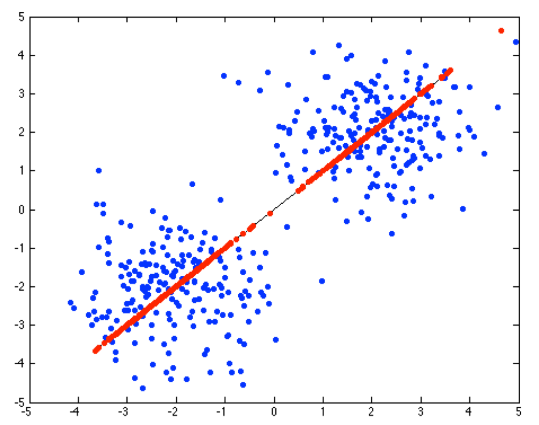
\includegraphics[width=.5\textwidth]{figures/pca-illustration.png}
    \caption{Illustration of PCA.}
    \label{pca_illustration}
\end{figure}

The PCA can be obtained through singular value decomposition. Recall that it is possible to represent any $\mathbf{X}\in\mathbb{R}^{n\times d}$ as $\mathbf{X=USV}^T$ where $\mathbf{U}\in\mathbb{R}^{n\times n}$ and $\mathbf{V}\in\mathbb{R}^{d\times d}$ are orthogonal, and $\mathbf{S}\in\mathbb{R}^{n\times d}$ is diagonal (wlog in decreasing order). Its entries are called singular values.

The top $k$ principal components are exactly the first $k$ columns of $\mathbf{V}$. Note that:
\begin{equation}
    n\Sigma=\mathbf{X}^T\mathbf{X}=\mathbf{US}^t\mathbf{U}^T\mathbf{USV}^T=\mathbf{VS}^T\mathbf{SV}^T
\end{equation}

Choosing $k$ for PCA can be done depending on the application domain:
\begin{itemize}
    \item For visualization: by inspection
    \item For feature induction: by cross-validation
    \item Otherwise: pick k so that most of the variance is explained.
\end{itemize}

Note that the PCA and the $k$-means problems are not very dissimilar. They both solve the following problem:
\begin{equation*}
    (\mathbf{W}, \mathbf{z}_1, \ldots, \mathbf{z}_n)=\arg\min\sum_{i=1}^{n}\norm{\mathbf{W}\mathbf{z}_i-\mathbf{x}_i}^2_2
\end{equation*}

Except that $\mathbf{W}$ in PCA is orthogonal, and arbitrary in $k$-means.
Additionally, $\mathbf{z}_1, \ldots, \mathbf{z}_n)\in\mathbb{R}^{d}$ in PCA and $\mathbf{z}_1, \ldots, \mathbf{z}_n)\in E_k$ where $E_k=\left\{[1,0,\ldots, 0],\ldots, [0,\ldots, 0, 1]\right\}$ is the set of unit vectors in $\mathbf{R}^d$

One can think of PCA and $k$-mans to solve a similar unsupervised learning problem with different constraints. Both aim to compress the data with maximum fidelity under constraints on model complexity, This insight gives rise to a much broader class of techniques, such as matrix factorization.

\subsection{Kernel PCA}

In order to reduce the dimensionality of data in higher dimensions in nonlinear forms, which can lead to significant loss of information as seen in figure \ref{failure_linear_feature_reduction}.

\begin{figure}
    \centering
    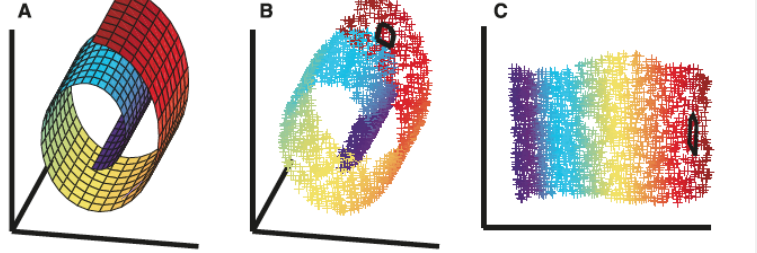
\includegraphics[width=.495\textwidth]{figures/failure_linear_feature_reduction.png}
    \hfill
    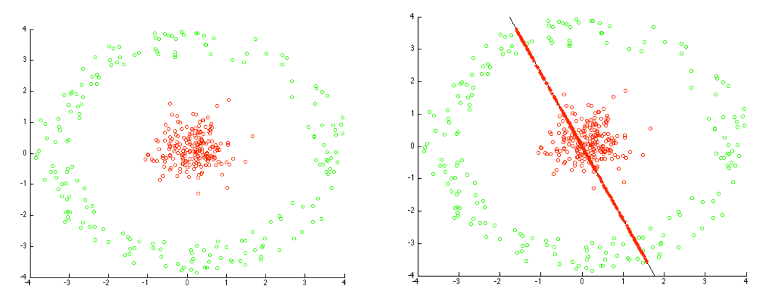
\includegraphics[width=.495\textwidth]{figures/failure_linear_feature_reduction_2.png}
    \caption{Linear feature reduction cannot reduce the dimensionality of this data very well.}
    \label{failure_linear_feature_reduction}
\end{figure}

Therefore we can use kernels. This way we can solve non-linear problems by reducing them to linear ones in high-dimensional, implicitely represented spaces. A similar approach for supervised learning can be taken.

The Ansatz we make is the following:
$\mathbf{w}=\sum_{i=1}^{n}\alpha_i\mathbf{x}_i$. For PCA, $w*$ is leading eigenvector of $\mathbf{X}^T\mathbf{X}$. We then have that $\mathbf{X}^T\mathbf{X}\mathbf{w}=\lambda\mathbf{w}$, therefore $\mathbf{w}=\frac{1}{\lambda}\sum_{i}$. If we define $\beta = \mathbf{X}\mathbf{w}$, we then have that $\mathbf{w}=\frac{1}{\lambda}\sum_{i}\beta_i x_i$ and $\alpha_i=\frac{\beta_i}{\lambda}$.

The objective we want to minimize is the following:
\begin{align*}
    \mathbf{w}^T\mathbf{X}^T\mathbf{X}\mathbf{w}&=\sum_{i=1}^{n}(\mathbb{W}^Tx_i)^2\\
    &=\sum_{i=1}^{n}((\sum_{j=1}^{n}\alpha_jx_j)^Tx_i)^2\\
    &=\sum_{i=1}^{n}(\sum_{j}\alpha_j(\mathbf{x}_j^T \mathbf{x}_i))^2\\
    &=\sum_{i=1}^{n}(\sum_{j}\alpha_j k(\mathbf{x}_j, \mathbf{x_i}))^2\\
    &=\sum_{i=1}^{n}(\alpha^T k_i)^2\\
    &=\alpha^T K^T K\alpha
\end{align*}

The constraints we want to put in place are the following:
\begin{align*}
    \norm{w}_2&=\mathbf{w}^T\mathbf{w}\\
    &=(\sum_{i=1}^{n}\alpha_i\mathbf{x}_i)^T(\sum_{j=1}^{n}\alpha_j\mathbf{x}_j)\\
    &=\sum_{ij}\alpha_i\alpha_j\mathbf{x}_i^T \mathbf{x}_j\\
    &=\sum_{ij}\alpha_i\alpha_jk(\mathbf{x}_i,\mathbf{x}_j)\\
    &=\alpha^T\mathbf{K}\alpha\stackrel{!}{=}1
\end{align*}

Thus, kernel PCA requires solving $\max_{\alpha}\alpha^T\mathbf{K}^T\mathbf{K}\alpha$ such that $\alpha^TK\alpha=1$.

Applying feature maps using:
\begin{equation*}
    \mathbf{w}=\sum_{j=1}^{n}\alpha_j\phi(\mathbf{x}_j)
\end{equation*}

and observing $\norm{\mathbf{w}}_2^2=\alpha^T\mathbf{K}\alpha$, we have that:
\begin{align*}
    \arg\max_{\norm{\mathbf{w}}_2^2=1}\sum_{i=1}^{n}(\mathbf{w}^T\phi(\mathbf{x}_i))^2&=\arg\max_{\alpha^T\mathbf{K}\alpha=1}\sum_{i=1}^{n}(\sum_{j=1}^{n}\alpha_j\phi(\mathbf{x}_j)^T\phi(\mathbf{x_i}))^2\\
    &=\arg\max_{\alpha^T\mathbf{K}\alpha=1}\sum_{i=1}^{n}(\sum_{j=1}^{n}\alpha_jk(\mathbf{x}_j, \mathbf{x}_i))^2\\
    &=\arg\max_{\alpha^T\mathbf{K}\alpha=1}\sum_{i=1}^{n}(\alpha^T\mathbf{K}_i)^2\\
    &=\arg\max_{\alpha^T\mathbf{K}\alpha=1}\sum_{i=1}^{n}(\alpha^T\mathbf{K}_i)^2\\
    &=\arg\max_{\alpha^T\mathbf{K}\alpha=1}\alpha^T\mathbf{K}^T\mathbf{K}\alpha.
\end{align*}

\subsubsection{Kernel PCA for $k=1$}

The Kernel-PCA problem ($k=1$) requires solving:
\begin{equation*}
    \alpha*=\arg\max_{\alpha^T\mathbf{K}\alpha=1}\alpha^T\mathbf{K}^T\mathbf{K}\alpha.
\end{equation*}

The optimal solution is obtained in closed form from the eigendecomposition of $\mathbf{K}$:
\begin{equation*}
    \alpha* = \frac{1}{\sqrt{\lambda_1}}\mathbf{v}_1
\end{equation*}

This scaling is useful because:
\begin{align*}
    \alpha^T\mathbf{K}\alpha &= \frac{1}{\sqrt{\lambda_1}}v_1^T\mathbf{K}\frac{1}{\sqrt{\lambda_1}}v_1\\
    &=\frac{1}{\lambda_1}\cdot v_1^T\mathbf{K}v_1\\
    &=\frac{1}{\lambda_1}v_1^T(\lambda_1v_1)\\
    &=v_1^Tv_1=1
\end{align*}
\begin{equation*}
    \mathbf{K}=\sum_{i=1}^{n}\lambda_i\mathbf{v}_i\mathbf{v}_i^T\qquad\lambda_1\geq\ldots\geq\lambda_d\geq0
\end{equation*}
Given this, a new projected point $\mathbf{x}$ is projected as $\mathbf{z}\in\mathbb{R}^{k}$ such that:
\begin{equation*}
    \mathbf{z}_i=\mathbf{w}^{(i)T}\mathbf{x}=(\sum_{j=1}^{n}\alpha_j^{(i)}\mathbf{x}_j)^T\mathbf{x}=\sum_{j=1}^{n}\alpha_j^{(i)}\mathbf{x}_j^T\mathbf{x}=\sum_{j=1}^{n}\alpha_j^{(i)}k(\mathbf{x}_j, x)
\end{equation*}

\subsubsection{Kernel PCA for any $0<k<d$}

For any $1\leq k<d$, the kernel principal components are given by $\alpha^{(1)},\ldots, \alpha^{(k)}\in\mathbb{R}^n$ where:
\begin{equation*}
    \alpha^{(i)}=\frac{1}{\sqrt{\lambda_i}}\mathbf{v}_i
\end{equation*}
is obtained from:
\begin{equation}
    \mathbf{K}=\sum_{i=1}^{n}\lambda_i\mathbf{v}_i\mathbf{v}_i^T\qquad\lambda_1\geq\ldots\geq\lambda_d\geq 0.
\end{equation}
Given this, a new point $\mathbf{x}$ is projected as $\mathbf{z}\in\mathbb{R}^k$:
\begin{equation*}
    z_i=\sum_{j=1}^{n}\alpha_j^{(i)}k(\mathbf{x}, \mathbf{x}_j)
\end{equation*}

Applying $k$-means on kernel principal components is sometimes called kernel-$k$-means or spectral clustering. The illustration of the advantage of kernelizing PCA is shown in figure \ref{kernelized_pca} and \ref{kernerlized_pca_2}.

\begin{figure}
    \centering
    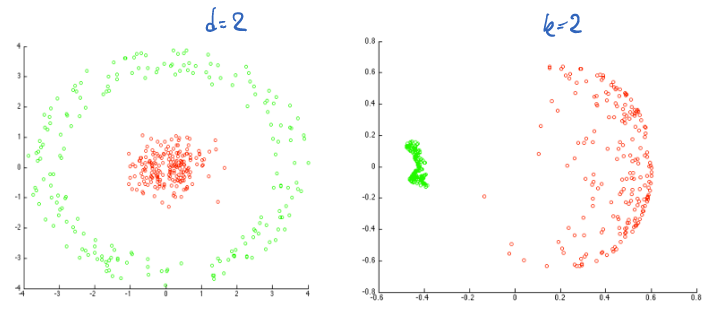
\includegraphics[width=.5\textwidth]{figures/kernelized_pca.png}
    \caption{Kernelized PCA illustration}
    \label{kernelized_pca}
\end{figure}

\begin{figure}
    \centering
    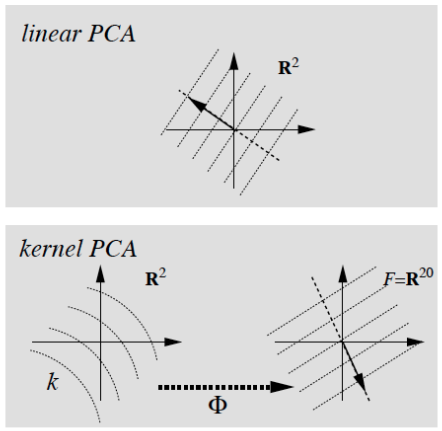
\includegraphics[width=.5\textwidth]{figures/kernerlized_pca_2}
    \caption{Another kernelized PCA illustration}
    \label{kernerlized_pca_2}
\end{figure}

Kernel-PCA corresponds to applying PCA in the feature space induced by the kernel $k$. It can be used to discover non-linear feature maps in closed form. This can be used as inputs, e.g. to SVMs given multi layer SVMs. The kernel could also be centered, i.e.:
\begin{equation*}
    \mathbf{K}'=\mathbf{K}-\mathbf{KE}-\mathbf{EK}+\mathbf{EKE}
\end{equation*}
and $\mathbf{E}=\frac{1}{n}[1,\ldots, 1][1,\ldots, 1]^T$

It should be noted that kernelized PCA requires data specified as kernel. The complexity grows with the number of datapoints and cannot be easily explicitely embed high-dimensional data unless we have an appropriate kernel, which may not always be the case. Alternatives include:
\begin{itemize}
    \item Autoencoders
    \item Locally linear embedding
    \item Multi-dimensional scaling
    \item t-SNE
\end{itemize}

\subsection{Neural network autoencoders}

The key idea behind autoencoders is to try to learn the identity function:
\begin{equation*}
    \mathbf{x}\approx f(\mathbf{x};\theta)
\end{equation*}
The function $f$ can be decomposed by an encoder and a decoder, $f_1$ and $f_2$ respectively:
\begin{equation*}
    f(\mathbf{x};\theta) = f_2(f_1(\mathbf{x};\theta_1);\theta_2)
\end{equation*}

Neural networks can be used to learn the parameters $theta$, as shown in figure \ref{autoencoder_network}.

\begin{figure}
    \centering
    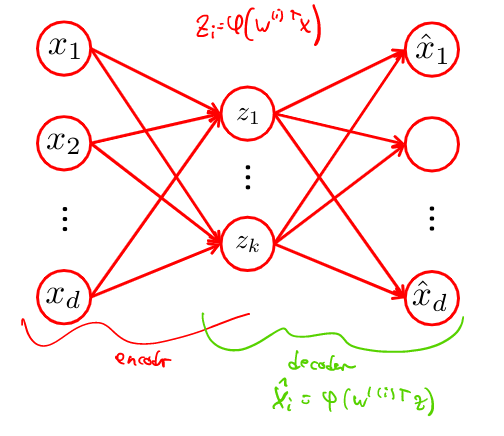
\includegraphics[width=.5\textwidth]{figures/autoencoder_network.png}
    \caption{An autoencoder network}
    \label{autoencoder_network}
\end{figure}

Neural network autoencoders are ANNs where there is one output unit for each of the $d$ input units. The number $k$ of hidden units is uually smaller than the number of inputs. The goal is to optimize the weights such that the output agrees with the input.

\subsubsection{Training autoencoders}

The goal is to optimize the weights such that the output agrees with the input. This entails, for instance, minimizing the squared loss:

\begin{equation*}
    \min_{\mathbf{W}}\sum_{i=1}^{n}\norm{\mathbf{x_i}-\mathbf{f}(\mathbf{x}_i;\mathbf{W})}_2^2=\min_{\mathbf{W}}\sum_{i=1}^{n}(\sum_{j=1}^{d}(\mathbf{x}_{i,j}-\mathbf{f}(\mathbf{x}_i;\mathbf{W}))^2)
\end{equation*}

The aim is to find a local minimum via SGD (backpropagation). The initialization of such networks matters and is challenging

\section{Probabilistic modelling}

The reason why we want to have a statistical perspective on supervised learning is that we want to quantify uncertainty, and express prior knowledge and assumptions about the data.

\subsection{Probabilistic interpretation of LSR}

We recall given $(\mathbf{x}_i, y_i)\sim P(\mathbf{X},Y)$, we wish to identify a hypothesis $h:\mathcal{X\rightarrow \mathcal{Y}}$ that minimizes the prediction error:
\begin{equation*}
    R(h) = \int P(\mathbf{x},y)\ell(y;h(\mathbf{x}))\text{d}\mathbf{x}\text{d}y=\mathbb{E}_{\mathbf{x},y}[\ell(y;h(\mathbf{x}))]
\end{equation*}
In least-squares regression, the risk is defined as:
\begin{equation*}
    R(h) = \mathbb{E}_{\mathbf{X},Y}[(Y-h(\mathbf{X}))^2]
\end{equation*}
Suppose we know $P(\mathbf{X},Y)$ (which is unrealistic), then $h$ is minimized by:
\begin{align*}
    \min_{h:\mathbb{R}^d\mathbb{R}}R(h)&=\min_{h}\mathbb{E}_{(\mathbf{x},y)\sim P}[(y-h(\mathbf{x}))^2]\\
    &= \min_{h}\mathbb{E}_{\mathbf{x}}[\mathbb{E}_y[(Y-h(\mathbf{x}))^2|\mathbf{X}=\mathbf{x}]]\\
    &= \mathbb{E}_{\mathbf{x}}[\min_{h(\mathbf{x})}\mathbb{E}_{y}[(Y-h(\mathbf{x}))^2|\mathbf{X}=\mathbf{x}]]
\end{align*}
Since we consider an arbitrary $h$, we choose $h(\mathbf{x})$ and $h(\mathbf{x'})$ independently for $\mathbf{x}\neq\mathbf{x}'$

In the context of least squares regression, the optimal prediction is given by:
\begin{equation*}
    y*(\mathbf{x})\in\arg\min_{\hat{y}}\mathbb{E}_{Y}[(\hat{y}-Y)^2|\mathbf{X}=\mathbf{x}]=\arg\min_{\hat{y}}\ell(\hat{y})
\end{equation*}
where $\ell(\hat{y})$ can be rewritten as:
\begin{equation*}
    \frac{d}{d\hat{y}}\ell(\hat{y}) = \int(\hat{y}-y)^2p(y|\mathbf{x})dy
\end{equation*}
In order to find the minimum of that function we find its derivative and set it to 0:
\begin{align*}
    \frac{d}{d\hat{y}}\ell(\hat{y}) &= \int \frac{d}{d\hat{y}}(\hat{y}-y)^2p(y|\mathbf{x})dy \\
    &= \int 2(\hat{y}-y)p(y|\mathbf{x})dy\overset{!}{=} 0\\
    &\Rightarrow\int\hat{y}p(y|\mathbf{x})dy=\int yp(y|\mathbf{x})dy \\
    &\Leftrightarrow \hat{y}=\mathbb{E}[Y|\mathbf{X}=\mathbf{x}]
\end{align*}

So, assuming the data is iid according to $(\mathbf{x}_iy_i)\sim P(\mathbf{X},Y)$, the hypothesis $h*$ minimizing $R(h)=\mathbb{E}_{\mathbf{x},y}[(y-h(\mathbf{x}))^2]$ is given by the conditional mean:
\begin{equation*}
    h*(\mathbf{x})=\mathbb{E}[Y|\mathbf{X}=\mathbf{x}]
\end{equation*}
This (in practice unattainable) hypothesis is called the Bayes optimal predictor for the squared loss. However in practice we have finite data. Thus, one strategy for estimating a predictor from training data is to estimate the conditional distribution:
\begin{equation*}
    \hat{P}(Y|\mathbf{X})
\end{equation*}
and then, for test point $\mathbf{x}$, we predict the label:
\begin{equation*}
    \hat{y}= \hat{\mathbb{E}}[Y|\mathbf{X}=\mathbf{x}]=\int\hat{P}(y|\mathbf{X}=\mathbf{x})ydy
\end{equation*}

\subsection{Estimating conditional distribution}

From the derivation above, we hence need to estimate $\hat{P}(Y|\mathbf{X}, \theta)$ and then we optimize the parameters using parametric estimation, specifically maximum likelihood estimation.

\begin{align*}
    \theta*&=\arg\max_{\theta}\hat{P}(y_1,\ldots, y_n|\mathbf{x}_1,\ldots, \mathbf{x}_n, \theta)\\
    &\overset{iid}{=}\arg\max_{\theta}\prod_{i=1}^n\hat{P}(y_i|\mathbf{x}_i,\theta)=\arg\max_{\theta}\log\prod_{i=1}^n\hat{P}(y_i|\mathbf{x}_i,\theta)\\
    &=\arg\max_{\theta}\sum_{i=1}^{n}\log\hat{P}(y_i|\mathbf{x}_i,\theta)=\arg\min_{\theta}-\sum_{i=1}^{n}\log\hat{P}(y_i|\mathbf{x}_i,\theta)
\end{align*}

\subsubsection{Conditional linear Gaussian}

Suppose we assume $Y=h(X)+\epsilon$, with $\epsilon\sim\mathcal{N}(0,\sigma^2)$. Additionally, we also assume $h(\mathbf{x})=\mathbf{w}^T\mathbf{x}$. Then, we have:
\begin{equation*}
    \hat{P}(Y=y|\mathbf{X},\mathbf{w},\sigma^2)=\mathcal{N}(y;\mathbf{w}^T\mathbf{x},\sigma^2)
\end{equation*}
and
\begin{align*}
    \hat{\mathbf{w}}&=\arg\max_{\mathbf{w}}\hat{P}(y_{1:n}|X_{1:n},\mathbf{w},\sigma^2)\\
    &=\arg\min_{\mathbf{w}}-\sum_{i=1}^{n}\log\hat{P}(y_i|x_i,\mathbf{w},\sigma^2)\\
\end{align*}

\subsection{Probabilistic model for regression}

Consider linear regression. Let's make the statistical assumption that the noise is Gaussian, i.e. that $y_i\sim\mathcal{N}(\mathbf{w}^T\mathbf{x}_i,\sigma^2)$. Then, we can compute the conditional likelihood of the data given any candidate model $\mathbf{w}$ as:
\begin{align*}
    -\log\hat{p}(y|X,\mathbf{w})&=-\log\mathcal{N}(y|\mathbf{w}^Tx,\sigma^2)=-\log(\frac{1}{\sqrt{2\pi\sigma^2}})\exp(-\frac{(y-\mathbf{w}^T\mathbf{x})^2}{2\sigma^2})\\
    &=\frac{1}{2}\log 2\pi\sigma^2+\frac{1}{2\sigma^2}(y-\mathbf{w}^T\mathbf{x})^2\\
    \Rightarrow\hat{\mathbf{w}}&=\arg\max_{\mathbf{w}}P(y_{1:n}|\mathbf{X}_{1:n},\mathbf{w},\sigma^2)=\arg\min_{\mathbf{w}}\sum_{i=1}^{n}(\frac{1}{2}\log2\pi\sigma^2+\frac{1}{2\sigma^2}(y_i-\mathbf{w}^T\mathbf{x}_i)^2)\\
    &=\arg\max_{\mathbf{w}}\frac{n}{2}\log 2\pi\sigma^2+\frac{1}{2\sigma^2}\sum_{i=1}^{n}(y_i-\mathbf{w}^T\mathbf{x}_i)^2=\arg\min_{\mathbf{w}}\sum_{i=1}^{n}(y_i-\mathbf{w}^T\mathbf{x}_i)^2
\end{align*}

The negative log likelihood for the conditional linear Gaussian is given by:
\begin{equation*}
    L(\mathbf{w})=-\log P(y_1,\ldots, y_n|\mathbf{x}_1,\ldots, \mathbf{x}_n,\mathbf{w}) = \frac{n}{2}\log(2\pi\sigma^2) + \sum_{i=1}^{n}\frac{(y_i-\mathbf{w}^T\mathbf{x}_i)^2}{2\sigma^2}
\end{equation*}
Thus, under the conditional linear Gaussian assumption, maximizing the likelihood is equivalent to least squares estimation, i.e.:
\begin{equation*}
    \arg\max_{\mathbf{w}}P(y_1, \ldots, y_n|\mathbf{x}_1, \ldots, \mathbf{x}_n, \mathbf{w})=\arg\min_{\mathbf{w}}\sum_{i=1}^{n}(y_i-\mathbf{w}^T\mathbf{x}_i)^2
\end{equation*}

More generally, the MLE for data with Gaussian iid noise can be derived as follows. Suppose $\mathcal{H}=\left\{h:\mathcal{X}\rightarrow\mathbb{R}\right\}$ is a class of functions. Assuming that $P(Y=y|\mathbf{X}=\mathbf{x})=\mathcal{N}(y|h*(\mathbf{x}),\sigma^2)$ for some function $h*:\mathcal{X}\rightarrow\mathbb{R}$ and some $\sigma^2>0$ the MLE for data $D=\left\{(\mathbf{x}_1, y_1), \ldots, (\mathbf{x}_n,y_n)\right\}$ in $\mathcal{H}$ is given by:
\begin{equation*}
    \hat{h}=\arg\min_{h\in\mathcal{H}}\sum_{i=1}^{n}(y_i-h(\mathbf{x}_i))^2
\end{equation*}

The fact that the MLE is given by the least squares solution, assuming that the noise is idd Gaussian with constant variance is useful since it satisfies several nice statistical properties:
\begin{description}
    \item[Consistency] Parameter estimate converges to true parameters in probability
    \item[Asymptotic efficiency] the smallest variance among all well-behaved estimators for large $n$.
    \item[Asymptotic normality]
\end{description}
However, all these properties are asymptotic. For finite $n$, we still need to be careful about overfitting.

\subsection{Bias variance tradeoff}
\begin{redbox}{}
    The bias variance tradeoff is defined as:
    \begin{equation*}
        \text{Prediction error} = \text{Bias}^2+\text{Variance} + \text{Noise}
    \end{equation*}
\end{redbox}
where:
\begin{description}
    \item[Bias]: Excess risk of best model considered compared to minimal achievable risk knowing $P(\textbf{X},Y)$, i.e. given infinite data.
    \item[Variance]: Risk incurred due to estimating model from limited data.
    \item[Noise]: Risk incurred by optimal model (i.e. irreducible error).
\end{description}

To investigate where bias comes from, the MLE solution depends on training data $D$:
\begin{equation*}
    \hat{h} = \hat{h}_D=\arg\min_{h\in\mathcal{H}}\sum_{(\mathbf{x},y)\in D}(y-h(\mathbf{x}))^2
\end{equation*}

But training data $D$ is itself random (drawn iid fro $P$). We might want to choose $H$ to have small bias (i.e., have small squared error on average, see red part of the equation below).
\begin{equation*}
    \mathbb{E}_{\mathbf{X}}[\mathcolor{red}{\mathbb{E}_D\hat{h}_D(\mathbf{X})-h*(\mathbf{X})}]^2
\end{equation*}

To see where variance comes from, the MLE solution depends on training data $D$:
\begin{equation*}
    \hat{h} = \hat{h}_D=\arg\min_{h\in\mathcal{H}}\sum_{(\mathbf{x},y)\in D}(y-h(\mathbf{x}))^2
\end{equation*}
This estimator is itself random, and has some variance:
\begin{equation*}
    \mathbb{E}_{\mathbb{X}}\text{Var}_D[\hat{h}_D(\mathbf{X})]^2 = \mathbb{E}_{\mathbb{X}}\mathbb{E}_{D}[\hat{h}_D(\mathbf{X})-\mathbb{E}_{D},\hat{h}_D,(\mathbf{X})]^2
\end{equation*}

Finally, even if we know the Bayes' optimal hypothesis h*, we'd still incur some error due to noise:
\begin{equation*}
    \mathbb{E}_{\mathbf{X},Y}[(Y-h*(\mathbf{X}))^2]
\end{equation*}
This error is irreducible, i.e., independent of the choice of the hypothesis class.

In summary:

\begin{align*}
    \mathcolor{BrickRed}{\mathbb{E}_D\mathbb{E}_{\mathbf{X},Y}[(Y-\hat{h}_D(\mathbf{X}))^2]} &= \mathbb{E}_{\mathbf{X}}[\mathcolor{NavyBlue}{\mathbb{E}_D\hat{h}_D(\mathbf{X})-h*(\mathbf{X})}]^2\\
    &+\mathcolor{ForestGreen}{\mathbb{E}_{\mathbf{X}}\mathbb{E}_D[\hat{h}_D(\mathbf{X})-\mathbb{E}_D,\hat{h}_D,(\mathbf{X})]^2}\\
    &+\mathcolor{magenta}{\mathbb{E}_{\mathbf{X},Y}[Y-h*(\mathbf{X})]^2}
\end{align*}

where the terms are \textcolor{BrickRed}{expected risk}, \textcolor{NavyBlue}{bias}, \textcolor{ForestGreen}{variance} and \textcolor{magenta}{noise} and ideally we wish to find an estimator that simultaneously minimizes bias and variance.

\subsection{Bias and variance in regression}

The MLE for linear regresison is unbiased (if $h*$ is in class $\mathcal{H}$). Furhtermore, it is the minimum variance estimator among all unbiased estimators according to the Gauss-Markov theorem. Hoever, we have already seen that the least-squares solution can overfit. Thus, it is sometimes important to trade some bias for a reduction of variance through regularization, like Ridge and Lasso.

\subsection{Bias in Bayesian modelling}

It is possible to introduce bias by expressing assumptions on parameters through a Bayesian prior. For example, let's assume $\mathbf{w}\sim\mathcal{N}(0,\beta^2\mathbf{I})$ which is equivalent to $w_i\sim\mathcal{N}(0,\beta^2)\forall i\in d$. Then, the posterior distribution of $\mathbf{w}$ is given using Bayes' rule by:
\begin{align*}
    P(\mathbf{w}|\mathbf{X}_{1:n}y_{1:n})&=\frac{P(\mathbf{w}|X_{1:n})P(y_{1:n}|w_1,\mathbf{X}_{1:n})}{P(y_{1:n}|\textbf{X}_{1:n})}\\
    &=\frac{P(\mathbf{w})P(y_{1:n}|w_1,\mathbf{X}_{1:n})}{P(y_{1:n}|\textbf{X}_{1:n})}
\end{align*}

The second line was obtained assuming the independence of $\mathbf{w}$ of $\mathbf{x}$. With this we can determine which parameters $\mathbf{w}$ are most likely a posteriori, which is equivalent to the maximum a posteriori estimate. I.e., given

\begin{equation*}
    P(\mathbf{w}|\mathbf{x}_1,\ldots, \mathbf{x}_n,y_1, \ldots, y_n) = \frac{P(\mathbf{w})P(y_1,\ldots,y_n|\mathbf{x}_1,\ldots,\mathbf{x}_n,\mathbf{w})}{P(y_1,\ldots,y_n|\mathbf{x}_1,\ldots, \mathbf{x}_n)}
\end{equation*}

we want:

\begin{equation}\label{mpebayes}
    \arg\max_{\mathbf{w}}P(\mathbf{w}|\mathbf{X}_{1:n},y_{1:n})=\arg\min_{\mathbf{w}}-\log P(\mathbf{w})-\log P(\mathbf{Y}_{1:n}|\mathbf{X}_{1:n},\mathbf{w}) + \log P(Y_{i:n}|X_{1:n})
\end{equation}

Note: we can neglect $\log P(Y_{i:n}|X_{1:n})$ because it is independent of $\mathbf{w}$.

\begin{align*}
    -\log P(\mathbf{w}) &= -\log \prod_{i=1}^d P(w_i) = -\sum_{i=1}^{d}\log\mathcal{N}(w_i;0,\beta^2)\\
    &=-\sum_{i=1}^{d}\log\frac{1}{\sqrt{2\pi\beta^2}}\exp(\frac{-w_i^2}{2\beta^2})=\frac{d}{2}\log 2\pi\beta^2+\frac{1}{2\beta^2}\sum_{i=1}^{d}w_i^2\\
    &=c+\frac{1}{2\beta^2}\norm{w}_2^2
\end{align*}

Coming back to equation to equation \ref{mpebayes}, we now can derive:

\begin{align*}
    (*) &= \arg\min_{\mathbf{w}}\frac{1}{2\beta^2}\norm{w}_2^2 + \frac{1}{2\beta^2}\sum_{i=1}^{n}(y_i-\mathbf{w}^Tx_i)^2\\
    &=\arg\min_{\mathbf{w}}\frac{\sigma^2}{\beta^2}\norm{\mathbf{w}}_2^2+\sum_{i=1}^{n}(y_i-\mathbf{w}x_i)^2
\end{align*}
which is equivalent to Ridge regression for $\lambda=\frac{\sigma^2}{\beta^2}$.

\subsection{Ridge regression is equivalent to MAP estimation}

Ridge regression can be understood as finding the MAP parameter estimate for a linear regression problem, assuming that the noise is iid Gaussian and the prior on the model parameters is Gaussian, i.e.:
\begin{equation*}
    \arg\min_{\mathbf{w}}\sum_{i=1}^{n}(y_i-\mathbf{w}^T\mathbf{x}_i)^2+\lambda\norm{\mathbf{w}}_2^2\equiv\arg\max_{\mathbf{w}}P(\mathbf{w})\prod_{i}P(y_i|\mathbf{x}_i,\mathbf{w})
\end{equation*}

More generally, regularized estimation can often be understood as MAP inference:
\begin{align*}
    \arg\min_{\mathbf{w}}\sum_{i=1}^{n}\ell(\mathbf{w}\mathbf{x}_i;\mathbf{x}_i, y_i)+C(\mathbf{w})&=\arg\max_{\mathbf{w}}\prod_i P(y_i|\mathbf{x}_i,\mathbf{w})P(\mathbf{w})\\
    &=\arg\max_{\mathbf{w}}P(\mathbf{w}|D)
\end{align*}
where $C(\mathbf{w})=-\log P(\mathbf{w})$ and $\ell(\mathbf{w}^T\mathbf{x}_i;\mathbf{x}_i,y_i)=-\log P(y_i|\mathbf{x}_i,\mathbf{w})$. This perspective allows changing priors ($\approx$ regularizers) and likelihoods ($\approx$ loss functions).

\subsection{L1-regularization}
The prior that corresponds to l1-regularization is the Laplace prior. Its shape can is depicted in figure \ref{laplaceprior} and is given in equation \ref{eq:laplaceprior}.

\begin{figure}[]
    \centering
    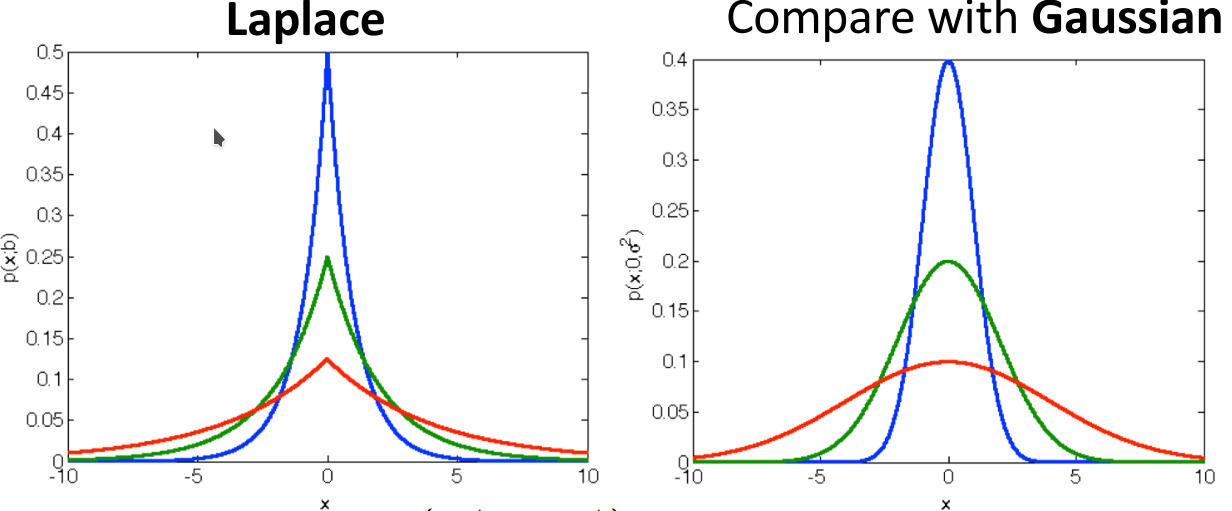
\includegraphics[width=.5\textwidth]{figures/laplaceprior.png}
    \caption{Laplace prior compared to the Gaussian prior.}
    \label{laplaceprior}
\end{figure}

\begin{equation}\label{eq:laplaceprior}
    p(x;\mu, b) = \frac{1}{2b}\exp(-\frac{|x-\mu|}{b})
\end{equation}

\subsection{Student-$t$ likelihood}
It is possible to introduce robustness by changing the likelihood (=loss) function, for instance using the non-standardized Student's-t likelihood given by:
\begin{equation*}
    P(y|\mathbf{x}, \mathbf{w},\nu,\sigma^2)=\frac{\Gamma (\frac{\nu+1}{2})}{\sqrt{\pi\nu\sigma^2}\Gamma(\frac{\nu}{2})}(1+\frac{(y-\mathbf{w}^T\mathbf{x})^2}{\nu\sigma^2})^{-\frac{\nu+1}{2}}
\end{equation*}

which yields heavier tails than normal distributions.

\subsection{Bayes' optimal predictor}

Assuming the data is generated iid, i.e. $(x_i, xy_i)\sim P(X,Y)$, the hypothesis $h^*$ $R(h) = \mathbb{E}[Y|\mathbf{X}=\mathbf{x}]$ is given by the conditional mean $h^*(x)=\mathbb{E}[Y|\mathbf{X}=\mathbf{x}]$ which is called the Bayes' optimal predictor for the squared loss. In this setting, one strategy for estimating a predictor from training data is to estimate the conditional distribution $\hat{P}(X|\mathbf{X})$ and then, for test point $\mathbf{x}$, the predicted label:
\begin{equation*}
  \hat{y} = \mathbb{\hat{E}}[Y|\mathbf{X}=\mathbf{x}] = \int\hat{P}(y|\mathbf{X}=\mathbf{x})ydy
\end{equation*}

Estimating the conditional distribution can be done using a common approach, which consists in (i) choose a particular parametric form from $\hat{P}(Y|\mathbf{X},\theta)$ and then optimize the parameters. This is done through maximum conditional likelihood estimation:
\begin{equation*}
  \theta^*=\arg\max_{\theta}\hat{P}(y_1,\ldots,y_n|\mathbb{x}_1,\ldots, \mathbf{x}_n,\theta)
\end{equation*}

In this context, Ridge regression can be understood as finding the MAP parameter estimate for a linear regression problem, assuming that:
\begin{itemize}
\item The noise $P(y|\mathbf{x},\mathbf{w})$ is iid Gaussian and
  \item The prior $P(\mathbf{w})$ on the model parameters $\mathbf{w}$ is Gaussian.
\end{itemize}

Then, we have the equivalence:
\begin{equation*}
  \arg\min_{\mathbf{w}}\sum_{i=1}^{n}(y_i-\mathbf{w}^T\mathbf{x}_i)^2 + \lambda\norm{\mathbf{w}}_2^2 \equiv\arg\max_{\mathbf{w}}P(\mathbf{w})\prod_iP(y_i|\mathbf{x}_i, \mathbf{w})
\end{equation*}

More generally, regularized estimation can often be understood as MAP inference:

\begin{align*}
  \arg\min_{\mathbf{w}}\sum_{i=1}^{n}\ell(\mathbf{w}^T\mathbf{x}_i;\mathbf{x}_i,y_i) + C(\mathbf{w}) &= \arg\max_{\mathbf{w}}\prod_i P(y_i|\mathbf{x}_i,\mathbf{w})P(\mathbf{w})\\
  &= \arg\max_{\mathbf{w}}P(\mathbf{w}|D)
\end{align*}

where $C(\mathbf{w})=-\log P(\mathbf{w})$ and $\ell(\mathbf{w}^T\mathbf{x}_i;\mathbf{x}_i,y_i) = -\log P(y_i|\mathbf{x}_i, \mathbf{w})$. This allows changing priors, which are equivalent to regularizers and likelihoods, which are equivalent to loss functions.

\subsection{Probablistic modelling (risk) in classification}

In classification, risk is defined as:
\begin{equation*}
  R(h) = \mathbb{E}_{\mathbf{X},Y}[[Y\neq h(\mathbf{X})]]
\end{equation*}

which is equal to 1 if $y\neq h(\mathbf{X})$ and 0 otherwise.

Now, suppose we know $P(\mathbf{X},Y)$, which $h$ minimizes the risk then?

\begin{equation*}
  h^*(\mathbf{x}) = \arg\min_{\hat{y}}\underbrace{\mathbb{E}[[Y\neq \hat{y}|\mathbf{X}=\mathbf{x}]]}_{\ell(\hat{y})}
\end{equation*}

Expanding $\ell(\hat{y})$ yields:

\begin{equation*}
  \ell(\hat{y}) = \sum_{y=1}^C P(Y=y|\mathbf{X}=\mathbf{x})[y\neq \hat{y}] = \sum_{y_i, y\neq\hat{y}}P(Y=y|\mathbf{X}=\mathbf{x})=1-P(Y=\hat{y}|\mathbf{X}=\mathbf{x})
\end{equation*}
So $h^*(\mathbf{x}) =\arg\max_{\hat{y}} P(Y=\hat{y}|\mathbf{X}=\mathbf{x})$.

In the context of logistic regression, we want to use a generalized linear model for the class probability. We know that $Y\in\left\{+1,-1\right\}$. The classification of a positive example is given by:
\begin{equation*}
  P(Y=1|\mathbf{x} = \sigma(\mathbf{w}^T\mathbf{x}))
\end{equation*}

where:

\begin{equation*}
  \sigma(z) = {1\over 1+\exp(-z)}
\end{equation*}

Note that this is equivalent to saying that $Y|\mathbf{X}=\mathbf{x}\sim\mathrm{Bernoulli} {(\sigma(\mathbf{w}^T\mathbf{x}))}$
The derivation of $P(Y=-1|\mathbf{X})$ is given below:

\begin{align*}
  P(Y=-1|\mathbf{x}) &= 1 - P(Y=1|\mathbf{x})\\
                     &= 1 - {1\over 1+\exp(-\mathbf{w}^T\mathbf{x})}\\
                     &= {\exp(-\mathbf{w}^T\mathbf{x})\over 1+\exp(-\mathbf{w}^T\mathbf{x})}\\
                     &= {1\over 1+\exp(\mathbf{w}^T\mathbf{x})}
\end{align*}
So, we get the general classification for $P(Y=y|\mathbf{x}) = {1\over 1+\exp(-y\cdot\mathbf{w}^T\mathbf{x})}$.

Logistic regression (a classification method) replaces the assumption of Gaussian noise (squared loss) by i.i.d. Bernoulli noise, and yields the following classification equation:

\begin{equation*}
  P(y|\mathbf{x},\mathbf{w}) = \mathrm{Bernoulli}(y;\sigma(\mathbf{w}^T\mathbf{x}))
\end{equation*}

vs.

\begin{equation*}
  P(y|\mathbf{x},\mathbf{w}) = \mathcal{N}(y;\mathbf{w}^T\mathbf{x}, \sigma^2)
\end{equation*}
for least squares regression. Similar to least square, the parameters $\mathbf{w}$ can be estimated using MLE or MAP.

The MLE for logistic regression is given by the following:

\begin{align}\label{eq:mle_logistic_regression}
  \hat{w} \in\arg\max_{\mathbf{w}} P(D|\mathbf{w})^{\text{iid}} &= \arg\max_{\mathbf{w}}\prod_{i=1}^{n}P(y_i|\mathbf{x}_i, \mathbf{w})\\
  &= \arg\min_{\mathbf{w}} - \sum_{i=1}^{n}\log P(y_i|x_i,\mathbf{w})\\
  &= \arg\min_{\mathbf{w}}\underbrace{\sum_{i-1}^{n}\underbrace{\log(1+\exp(-y_i\mathbf{w}^T\mathbf{x}_i))}_{\ell_{\text{logistic}}(\mathbf{w};\mathbf{x}_i,y_i)}}_{\hat{R}(\mathbf{w})}
\end{align}

Where the loss function we're trying to optimize is given by the following:

\begin{equation*}
  -\log P(y_i|\mathbf{x}_i,\mathbf{w}_i) = -\log{1\over 1+\exp(-y\mathbf{w}^T\mathbf{x}_i)} = \log (1+\exp(-y\mathbf{w}^T\mathbf{x}_i))
\end{equation*}

Plugging this result back into equation~\ref{eq:mle_logistic_regression} yields:

\begin{equation*}
  P(y_i|\mathbf{x}_i,\mathbf{w}) = {P(y_i,\mathbf{x}_i|\mathbf{w})\over P(\mathbf{x}_i,\mathbf{y})} \underbrace{= C_i P(y_i,x_i|\mathbf{w})}_{\text{if }P(\mathbf{x}_i|\mathbf{w})=P(\mathbf{x}_i)\rightarrow \mathbf{x}\text{ independent of }\mathbf{w}}
\end{equation*}

So, the negative log likelihood, which is equivalent to our objective function, is given by:
\begin{equation*}
  \hat{R}(\mathbf{w})=\sum_{i=1}^{n}\log(1+\exp(-y_i\mathbf{w}^T\mathbf{x}_i))
\end{equation*}
which is a convex function, which means that we can use convex optimization techniques like SGD.

Comparing the logistic loss to other loss functions already reviewed yields Figure~\ref{fig:comparison_loss_function}.

\begin{figure}
  \centering
  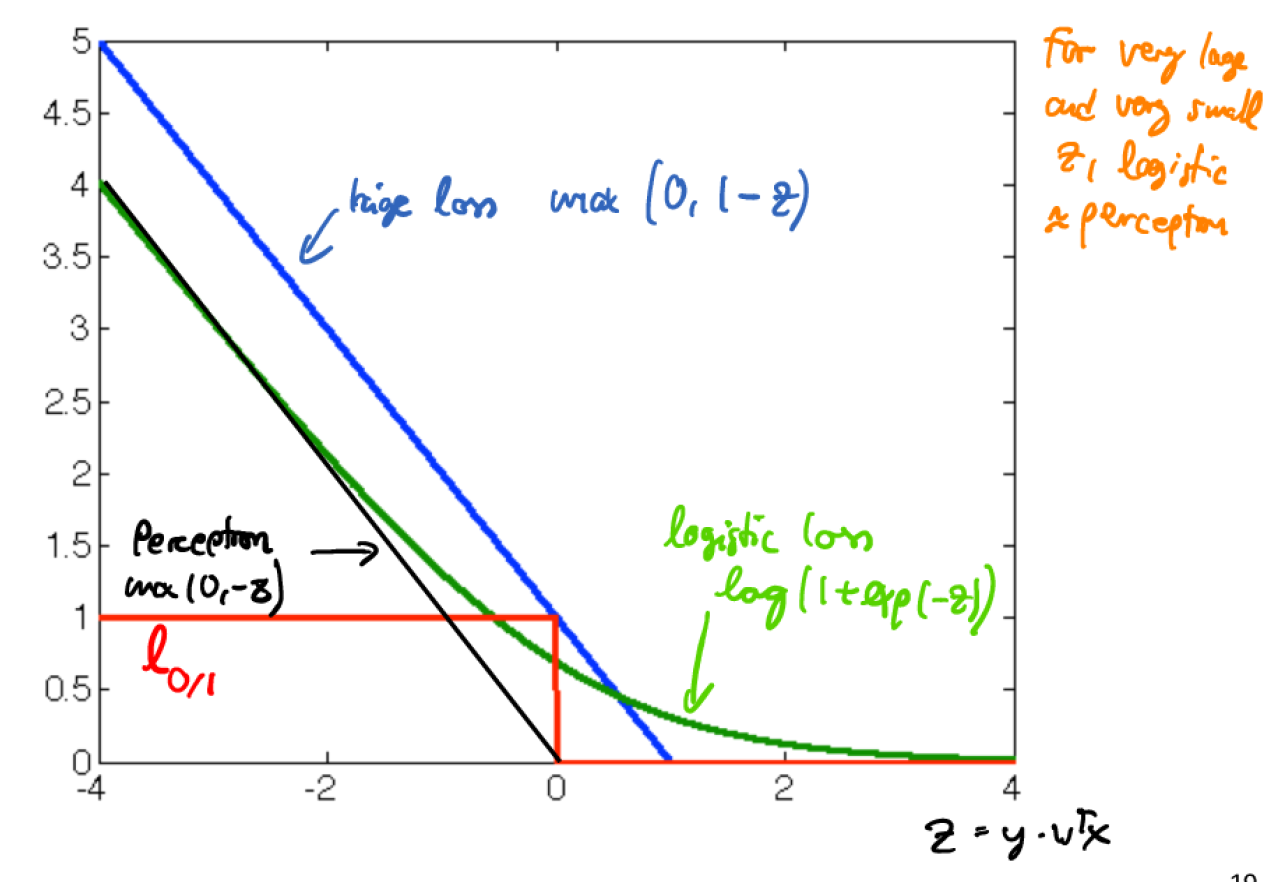
\includegraphics[width=0.5\textwidth]{figures/loss_functions.png}
  \caption{Comparing logistic loss to other loss functions.}
  \label{fig:comparison_loss_function}
\end{figure}

The loss for a data point $(\mathbf{x},y)$ is defined by:
\begin{equation*}
  \ell(\mathbf{w}) = \log(1+\exp(-y\mathbf{w}^T\mathbf{x}))
\end{equation*}
and its gradient is defined by:
\begin{align*}
  \nabla_{\mathbf{w}}\ell(\mathbf{w}) &= {1\over 1+\exp(-y\mathbf{w}^T\mathbf{x})}\cdot\exp(-y\mathbf{w}^T\mathbf{x})\cdot (-y\cdot\mathbf{x})\\
  &= {\exp(-y\mathbf{w}^T\mathbf{x})\over 1 + \exp(-y\mathbf{w}^T\mathbf{x})}(-y\cdot\mathbf{x})\\
  &= \underbrace{{1\over 1 + \exp(y\mathbf{w}^T\mathbf{x})}}_{P(Y\neq y|\mathbf{x})}(-y\cdot\mathbf{x})
\end{align*}

Once the gradient is defined, we can use SGD for logistic regression. The steps are:
\begin{enumerate}
  \item Initialize $\mathbf{w}$
  \item For $t=1,2,\ldots$:
    \begin{enumerate}
    \item Pick data point $(\mathbf{x},y)$ uniformly at random from data $D$.
    \item We compute the probability of misclassification with the current model, equivalent to:
        \begin{equation*}
          \hat{P}(Y=-y|\mathbf{w},\mathbf{x}) = {1\over 1+\exp(y\mathbf{w}^T\mathbf{x})}
        \end{equation*}
     \item Take a gradient step:
       \begin{equation*}
         \mathbf{w}\leftarrow\mathbf{w}+\eta_ty\mathbf{x}\hat{P}(Y=-y|\mathbf{w},\mathbf{x})
       \end{equation*}
    \end{enumerate}
\end{enumerate}

To control model complexity, regularization is desired. Thus, instead of solving the MLE, which corresponds to:
\begin{equation*}
  \min_{\mathbf{w}}\sum_{i=1}^n(\log(1+\exp(-y_i\mathbf{w}^T\mathbf{x}_i)))
\end{equation*}
we solve the regularized problem, which corresponds to either the Gaussian prior (L2):
\begin{equation*}
  \min_{\mathbf{w}}\sum_{i=1}^n\log(1+\exp(-y_i\mathbf{w}^T\mathbf{x}_i))+\lambda\norm{\mathbf{w}}_2^2
\end{equation*}
or Laplacian prior (L1):
\begin{equation*}
  \min_{\mathbf{w}}\sum_{i=1}^n\log(1+\exp(-y_i\mathbf{w}^T\mathbf{x}_i))+\lambda\norm{\mathbf{w}}_1
\end{equation*}

For L2-regularized SGD we add the following:

\begin{enumerate}
  \item Initialize $\mathbf{w}$
  \item For $t=1,2,\ldots$:
    \begin{enumerate}
    \item Pick data point $(\mathbf{x},y)$ uniformly at random from data $D$.
    \item We compute the probability of misclassification with the current model, equivalent to:
        \begin{equation*}
          \hat{P}(Y=-y|\mathbf{w},\mathbf{x}) = {1\over 1+\exp(y\mathbf{w}^T\mathbf{x})}
        \end{equation*}
     \item Take a gradient step:
       \begin{equation*}
         \mathbf{w}\leftarrow\mathbf{w}\textcolor{blue}{(1-2\lambda\eta_t)}+\eta_ty\mathbf{x}\hat{P}(Y=-y|\mathbf{w},\mathbf{x})
       \end{equation*}
    \end{enumerate}
\end{enumerate}

In summary regularized logistic regression has two steps:
\begin{itemize}
\item Learning
  \begin{itemize}
  \item Find optimal weights by minimizing logistic loss + regularizer, equivalent to:
  \begin{equation*}
    \hat{\mathbf{w}} = \arg\min_{\mathbf{w}}\sum_{i=1}^{n}\log(1+\exp(-y_i\mathbf{w}^T\mathbf{x}_i))+\lambda\norm{\mathbf{w}}_2^2
    = \arg\max_{\mathbf{w}}P(\mathbf{w}|\mathbf{x}_1,\ldots,\mathbf{x}_n,y_1,\ldots,y_n)
  \end{equation*}
  \end{itemize}
\item Classification
  \begin{itemize}
  \item Use a conditional distribution:
    \begin{equation*}
      \hat{P}(y|\mathbf{x},\hat{\mathbf{w}}) = {1\over 1+\exp(-y\hat{\mathbf{w}}^T\mathbf{x})}
    \end{equation*}
  \item Then, it's possible to predict the more likely class label:
  \begin{equation*}
    \hat{y}=\sigma(\hat{\mathbf{w}}^T\mathbf{x})
  \end{equation*}
  \end{itemize}
\end{itemize}

Let us derive that last result:
\begin{align*}
  \arg\max_{\hat{y}}P(\hat{y}|\mathbf{x},\hat{\mathbf{w}}) &=\arg\max_{\hat{y}}{1\over 1+\exp(-\hat{y}\hat{\mathbf{w}}^T)}\\
  &=\arg\min_{\hat{y}}\exp(-\hat{y}\hat{\mathbf{w}}^T\mathbf{x}) \\
  &=\arg\min_{\hat{y}}-\hat{y}\hat{\mathbf{w}}^T\mathbf{x}\\
  &=\arg\min_{\hat{y}\in\{+1,-1\}}-\hat{y}\hat{\mathbf{w}}^T\mathbf{x}=\sigma(\mathbf{w}^T\mathbf{x})
\end{align*}

Additional desirable features of logistic regression:
\begin{itemize}
\item Can kernelize
\item Can apply logistic loss function to neural networks in order to have them output probabilities
\item Natural multi-class variants
\end{itemize}

For the kernelized logistic regression, we follow these steps:
\begin{itemize}
\item Learning:
  \begin{itemize}
  \item Find optimal weights by minimizing logistic loss + regularizer
    \begin{equation*}
      \hat{\alpha} = \arg\min_{\alpha}\sum_{i=1}^{n}\log(1+\exp(-y_i\alpha^T\mathbb{K}_i))+\lambda\alpha^T\mathbf{K}\alpha
    \end{equation*}
    where $\mathbf{K} = (\mathbf{K}_1|\ldots|\mathbf{K}_n)$
  \end{itemize}
  \item Classification:
    \begin{itemize}
    \item Use conditional distribution
      \begin{equation*}
        \hat{P}(y|\mathbf{x},\hat{\mathbf{w}}) = {1\over 1+\exp(-y\sum_{j=1}^{n}\alpha_jk(\mathbf{x}_j,\mathbf{x}))}
    \end{equation*}
    \item Predict the most likely label
    \end{itemize}
  \end{itemize}

We can further extend multi-class logistic regression to a multi-class setting by maintaining one weight vector per class and model. We then have:

\begin{equation*}
  P(Y=i|\mathbf{x}, \mathbf{w}_1, \ldots, \mathbf{w}_c) = \underbrace{{\exp(\mathbf{w}_i^T\mathbf{x})\over \sum_{j=1}^{c}\exp(\mathbf{w}_j^T\mathbf{x})}}_{\hat{p}_i}
\end{equation*}

By default these weight vectors are not unique, and it is possible to force uniqueness by setting $w_c=0$, which recovers logistic regression as a special case.

The corresponding function (cross-entropy loss) is equivalent to:
\begin{equation*}
  \ell(y;\mathbf{x}, \mathbf{w}_1,\ldots,\mathbf{w}_c)=-\log P(Y=y|\mathbf{x}, \mathbf{w}_1, \ldots, \mathbf{w}_c)
\end{equation*}

The multiclass classification illustration is shown in figure

\begin{figure}
  \centering
  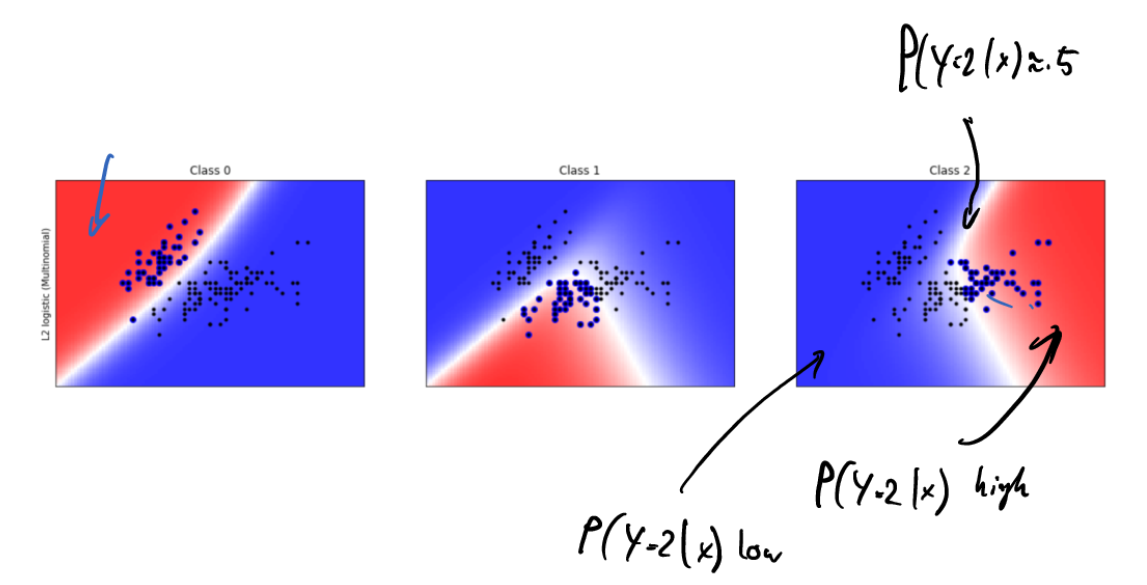
\includegraphics[width=.5\textwidth]{figures/multiclass-classification-probabilistic-interpretation.png}
  \caption{Multiclass classification with a probabilistic interpretation.}
  \label{fig:multiclass-classification-probabilistic-interpretation}
\end{figure}

Side note: training a neural network with multiple classes entails having multiple outputs and then compute the cross-entropy loss as well:
\begin{equation*}
  \ell(Y=i;f_1,\ldots, f_c) = -\log{\exp (f_i)\over \sum_{j=1}^{c}\exp(f_i)}
\end{equation*}

\begin{table}
  \centering
  \begin{tabular}{lll}
    \toprule
    Method & SVM/Perceptron & Logistic regression\\
    \midrule
    Advantages & Sometimes higher classification accuracy; Sparse sol's & Can obtain probabilities\\
    Disadvantages & Can't easily get class probabilities & Dense solutions\\
    \bottomrule
  \end{tabular}
  \caption{(Dis)advantages in SVM vs. logistic regression}
\end{table}

\subsection{Bayesian Learning Theory}

In the context of Bayesian decision theory, we consider the following. Given:
\begin{itemize}
\item A conditional distribution over labels $P(y|\mathbf{x})$ where $y\in\mathcal{Y}$ and $\mathcal{Y}$ can either be ${+1,-1}$, ${1,\ldots, c}$, $\mathbb{R}$
\item A set of actions $\mathcal{A}$ where $\mathcal{A}\neq\mathcal{Y}$
\item A cost function $C:\mathcal{Y}\times\mathcal{A}\rightarrow\mathbb{R}$
\end{itemize}
Bayesian decision theory recommends to pick the action that minimizes the expected cost:

\begin{equation*}
  a^*= \arg\min_{a\in\mathcal{A}}\mathbb{E}_y[C(y,a)|\mathbf{x}]
\end{equation*}

If we had access to the true distribution $P(y|\mathbf{x})$ this implements the Bayesian optimal decision. In practice, however, we can only estimate the distribution using e.g. logistic regression.

Making the optimal decision for logistic regression is achieved as follows:
\begin{itemize}
\item We have an estimated conditional distribution:
  \begin{equation*}
    \hat{P}(y|\mathbf{x})=\mathrm{Bernoulli}(y;\sigma(\hat{\mathbf{w}}^T\mathbf{x}))
  \end{equation*}
\item An action set:
  \begin{equation*}
    \mathcal{A} = {+1,-1}
  \end{equation*}
\item A cost function:
  \begin{equation*}
    C(y,a)=\underbrace{[y\neq a]}_{
      \begin{cases}
        1\text{ if }y\neq0\\
        0\text{ otherwise}
      \end{cases}
    }
  \end{equation*}
\item Then the action that minimizes the expected cost
  \begin{equation*}
    a^*=\arg\min_{a\in\mathcal{A}}\mathbb{E}_y[C(y,a)|\mathbf{x}] = \sum_yP(y|\mathbf{x})[y\neq a] = {1\over a+\exp(a\cdot \mathbf{w}^T\mathbf{x})}
  \end{equation*}
  is the most likely class:
  \begin{align*}
    a^*&=\arg\max_y\hat{P}(y|\mathbf{x})=\text{sign}(\mathbf{w}^T\mathbf{x})\\
  \end{align*}
  \begin{proof}
    \begin{align*}
      a^* &=\arg\min_a{1\over 1+\exp(a\mathbf{w}^T\mathbf{x})}\\
          &=\arg\max_a 1+\exp(a\mathbf{w}^T\mathbf{x})\\
          &=\arg\max_{a\in\{-1,+1\}} 1+\exp(a\mathbf{w}^T\mathbf{x})\\
          &=\arg\max_y\hat{P}(y|\mathbf{x})=\text{sign}(\mathbf{w}^T\mathbf{x})\\
    \end{align*}
  \end{proof}
\end{itemize}

For asymmetric costs, we amend the procedure as follows:
\begin{enumerate}
\item Estimated conditional distribution
  \begin{equation*}
    \hat{P}(y|\mathbf{x})=\mathrm{Bernoulli}(y;\sigma(\hat{\mathbf{w}}^T\mathbf{x}))
  \end{equation*}
\item An action set:
  \begin{equation*}
    \mathcal{A} = {+1,-1}
  \end{equation*}
\item A cost function:
  \begin{equation*}
    C(y,a)=
    \begin{cases}
      c_{FP}\quad\text{if }y=-1\text{ and }a=+1\\
      c_{FN}\quad\text{if }y=+1\text{ and }a=-1\\
      0\qquad\text{otherwise}
    \end{cases}
  \end{equation*}
\item Then the action that minimizes the expected cost is:
  \begin{align*}
    c_+ = \mathbb{E}_y[C(y,+1)|\mathbf{x}] &= P(y=-1|\mathbf{x})\cdot c_{FP}+\underbrace{P(y=+1|\mathbf{x})}_{p}\cdot 0\\
                                           &=(1-p)\cdot c_{FP}\\
    c_- = \mathbb{E}_y[C(y,-1)|\mathbf{x}] &= p\cdot C_{FN}+(1-p)\cdot 0 = p\cdot C_{FN}
  \end{align*}
\end{enumerate}
In this context, if we predict +1, we can derive the following:
\begin{align*}
  \text{predict }+1 &\Leftrightarrow c_+ < c_-\\
                    &\Leftrightarrow (1-p) c_{FP}<p c_{FN}\\
                    &\Leftrightarrow p>{C_{FP}\over C_{FP}+C_{FN}}
\end{align*}

Asymmetric costs are shown in Figure~\ref{fig:asymmetric_costs}

\begin{figure}
  \centering
  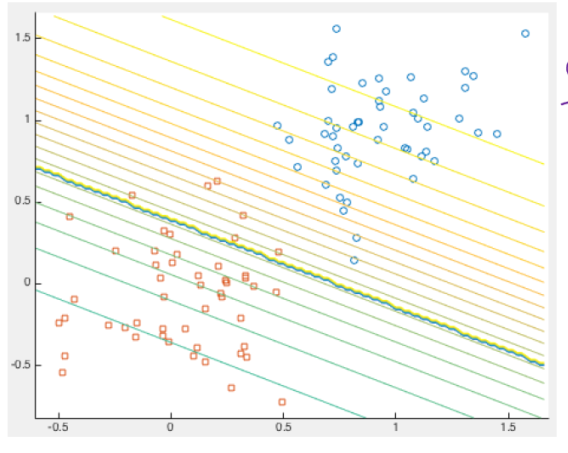
\includegraphics[width=0.5\textwidth]{figures/asymmetric_cost.png}
  \caption{Asymetric cost illustration}
  \label{fig:asymmetric_costs}
\end{figure}

It's also possible to made a ``doubtful'' logistic regression by making the following adjustments to the steps described above:

\begin{itemize}
\item We have an estimated conditional distribution:
  \begin{equation*}
    \hat{P}(y|\mathbf{x})=\mathrm{Bernoulli}(y;\sigma(\hat{\mathbf{w}}^T\mathbf{x}))
  \end{equation*}
\item An action set:
  \begin{equation*}
    \mathcal{A} = {+1,-1, D}
  \end{equation*}
\item A cost function:
  \begin{equation*}
    C(y,a)=
    \begin{cases}
      [y\neq a]\quad\text{if }a\in\{+1,-1\}\\
      c\quad \text{if } a=D
    \end{cases}
  \end{equation*}
\item Then the action that minimizes the expected cost
  \begin{equation*}
    a^*=\arg\min_{a\in\mathcal{A}}\mathbb{E}_y[C(y,a)|\mathbf{x}]
  \end{equation*}
  is given by:
  \begin{equation*}
    a^*=
    \begin{cases}
      y\quad\text{if }\hat{P}(y|\mathbf{x})\geq 1-c\\
      D\quad\text{otherwise }

    \end{cases}
  \end{equation*}
\end{itemize}
This corresponds to picking a given class if confidence enough.

\begin{figure}
  \centering
  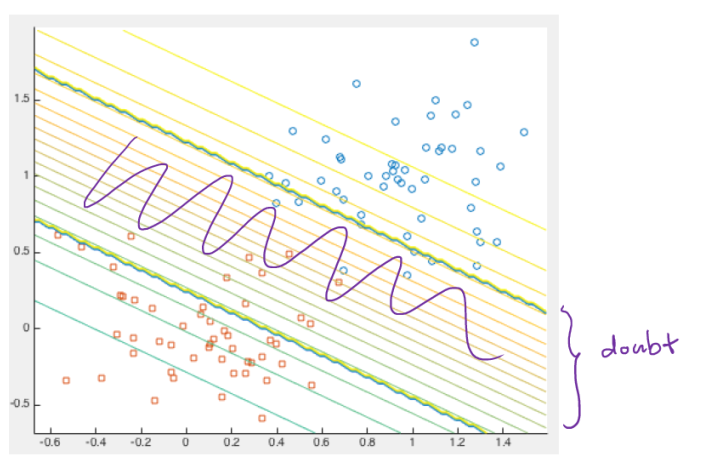
\includegraphics[width=0.5\textwidth]{figures/doubtful_classification.png}
  \caption{Area of doubt in doubtful logistic regression/}
  \label{fig:doubt_doubtful_classification}
\end{figure}

For least squares, the optimal decision is given by:

\begin{itemize}
\item Estimated conditional distribution
  \begin{equation*}
    \hat{P}(y|\mathbf{x})=\mathcal{N}(y;\hat{\mathbf{w}}^T\mathbf{x},\sigma^2)
  \end{equation*}
\item Action set is $\mathcal{A}=\mathbb{R}$
\item Cost function: $C(y,a)=(y-a)^2$
\item Then the action that minimizes the expected cost is:
  \begin{equation*}
    a^*=\arg\min_{a\in\mathcal{A}}\mathbb{E}_y[C(y,a)|\mathbf{x}]
  \end{equation*}
  is the conditional mean:
  \begin{align*}
    a^*&=\mathbb{E}_y[y|\mathbf{x}]=\int\hat{P}(y|\mathbf{x})dy\\
    &=\hat{\mathbf{w}}^T\mathbf{x}
  \end{align*}
\end{itemize}

And the asymmetric cost for regression is given by:

\begin{itemize}
\item Estimated conditional distribution
  \begin{equation*}
    \hat{P}(y|\mathbf{x})=\mathcal{N}(y;\hat{\mathbf{w}}^T\mathbf{x},\sigma^2)
  \end{equation*}
\item Action set is $\mathcal{A}=\mathbb{R}$
\item Cost function:
  \begin{equation*}
    C(y,a) = c_1\underbrace{\max(y-a,0)}_{underestimation}+c_@\underbrace{\max(a-y,0)}_{overestimation}
  \end{equation*}
  $=(y-a)^2$
\item Then the action that minimizes the expected cost is:
  \begin{equation*}
    a^*=\arg\min_{a\in\mathcal{A}}\mathbb{E}_y[C(y,a)|\mathbf{x}]
  \end{equation*}
  is:
  \begin{equation*}
    a^*= \hat{\mathbf{w}}^T\mathbf{x}+\sigma\cdot\phi^{-1}({c_1\over c_1+c_2})
  \end{equation*}
where $\phi^{-1}$ is the inverse Gaussian CDF.
\end{itemize}

\begin{figure}
  \centering
  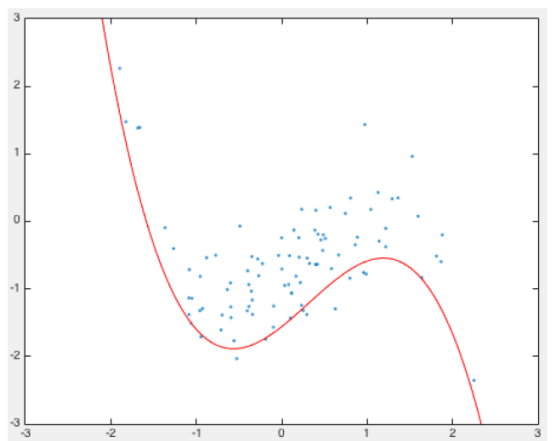
\includegraphics[width=0.5\textwidth]{figures/asymmetric_cost_regression.png}
  \caption{Asymmetric costs for regression}
  \label{fig:asymmetric_costs_for_regression}
\end{figure}

Note: asking an expert for labels is expensive, so we want to minimize the number of labels. A strategy to pick the examples we are most uncertain about is called uncertainty sampling.

\begin{itemize}
\item Given $D={(\mathbf{x}_i, \mathbf{y}_i)}^{n}_{i=1}$ you estimate $\hat{P}(y|\mathbf{x})$
\item For every $t=1,2,3,\ldots$:
  \begin{equation*}
    \hat{P}(y_i|\mathbf{x}_i)
  \end{equation*}
  given data $D$.
\item we pick the sample we are most uncertain about:
  \begin{equation*}
    i_t\in\arg\min_i|0.5-\hat{P}(Y_i|\mathbf{x}_i)|
  \end{equation*}
\item We query the label $y_{it}$, and set $D\leftarrow D\cup\{(\mathbf{x}_{i_t},y_{i_t})\}$
\end{itemize}

An example of obtaining the uncertainty score $u_j$ in logistic regression is:
\begin{equation*}
  u_j=-|\mathbf{w}^T\mathbf{x}_j|
\end{equation*}

Note that active learning and uncertainty sampling violate the i.i.d. assumption. It's also possible to get stuck with bad models. More advanced selection criteria are available.

Bayesian decision theory provides a principled way to derive decision rules from conditional distributions.

It can accomodate more complex settings like doubt, asymmetric losses, and active learning.

In summary:
\begin{enumerate}
\item Start with statistical assumptions on data. These data points are modeled iid but can be relaxed.
\item Choose likelihood function, e.g. Gaussian, student-t, logistic, exponential
\item We choose a prior, e.g. Gaussian, Laplace, exponential
\item Optimize for MAP parameters
\item Choose hyperparameters (variance, etc) through cross-validation.
\item Make predictions via BDT.
\end{enumerate}

\section{Discriminative vs. Generative modelling}

\subsection{Motivating example}

So far, we have considered only methods that estimate conditional distributions:
\begin{equation*}
  P(y|\mathbf{x})
\end{equation*}

Examples: linear regression, logistic regression, etc...

Such models do not attempt to model $P(\mathbf{x})$. Thus, they will not be able to detect outliers, i.e. unusual points for which $P(\mathbf{x})$ is very small.

The crucial difference between discriminative and generative modelling is the following. In discriminative models, we estimate:
\begin{equation*}
  P(y|\mathbf{x})
\end{equation*}
and in generative models, we seek to estimate the joint distribution
\begin{equation*}
  P(y,\mathbf{x})
\end{equation*}
It is possible to derive the conditional distribution from the joint distribution, but not vice versa.
\begin{equation*}
  (y|\mathbf{x}) \rightarrow P(y|\mathbf{x})={P(\mathbf{x}, y)\over P(\mathbf{x})}
\end{equation*}
where:
\begin{equation*}
  P(\mathbf{x}) = \sum_{y'}P(\mathbf{x}, y')
\end{equation*}

The typical approach for generative modelling is to follow these steps:
\begin{enumerate}
\item Estimate priors on labels $P(y)$\footnote{Mind the chain rule in probabilities: $P(\mathbf{x},y)=P(\mathbf{x}|y)P(y)=P(y|\mathbf{x})P(\mathbf{x})$}
\item Estimate the conditional distribution $P(\mathbf{x}|y)$ for each class $y$.
\item Obtain predictive distribution using Bayes' rule:
  \begin{equation*}
    P(y,\mathbf{x})=\underbrace{{1\over Z}}_{P(\mathbf{x})}\underbrace{P(y)P(\mathbf{x}|y)}_{P(y,\mathbf{x})}
  \end{equation*}
\end{enumerate}

Generative modeling attempts to infer the process, according to which examples are generated ($P(\mathbf{x},y)$). First, we generate class label $P(y)$. Then, we generate features given class $P(\mathbf{x}|y)$. An example of generative modelling is shown in figure~\ref{fig:example_generative_modelling}.

\begin{figure}
  \centering
  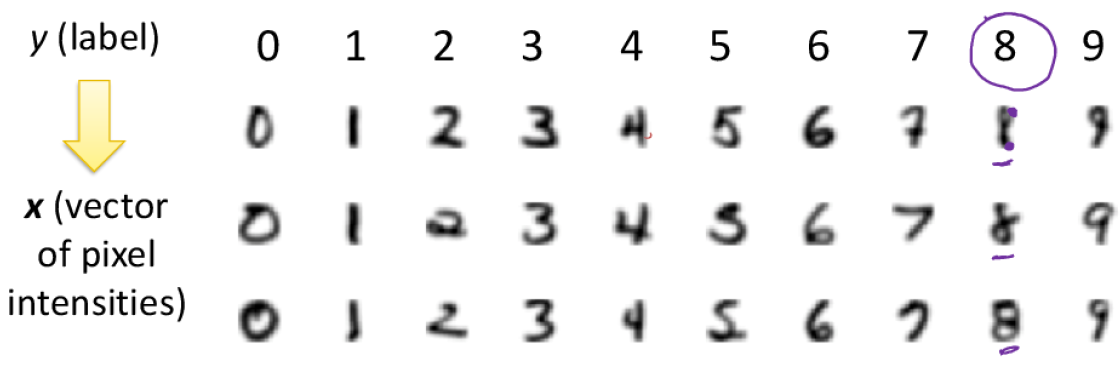
\includegraphics[width=0.5\textwidth]{figures/example_generative_modelling.png}
  \caption{Example of a generative model setting, producing handwritten digits.}
  \label{fig:example_generative_modelling}
\end{figure}

Gaussian naive Bayes classifiers:
\begin{description}
\item[Learning] Given data $\mathcal{D}=\{(\mathbf{x}_1,y_1),\ldots,(\mathbf{x}_n,y_n)\}$ we compute:
\begin{itemize}
\item MLE for class prior: $\hat{P}(Y=y)=\hat{p}_y={\text{Count}(Y=y)\over n}$
\item MLE for feature distribution:
  \begin{equation*}
    \hat{P}(x_i|y)=\mathcal{N}(x_i;\mu_{y,i}\sigma^2_{y,i})
  \end{equation*}
  \begin{align*}
    \hat{\mu}_{y,i}&={1\over\text{Count}(Y=y)}\sum_{j:y_j=y}\underbrace{x_{j,i}}_{\text{the value of feature }i\text{ for instance } j(x_j,y_j)}\\
    \hat{\sigma}^2_{y,i}&={1\over \text{Count}(Y=y)}\sum_{j:y_j=y}(x_{j,i}-\hat{\mu}_{y,i})^2
  \end{align*}
\item Prediction given a new point $\mathbf{x}$:
  \begin{equation*}
    y=\arg\max_{y'}\hat{P}(y'|\mathbf{x})=\arg\max\hat{P}(y')\prod_{i=1}^{d}\hat{P}(x_i|y')
  \end{equation*}
\end{itemize}
An example of decision boundaries under the following conditions:

\begin{equation*}
  \begin{cases}
    d=1\quad\text{1 feature }x\\
    \mathcal{Y}=\{-1,+1\}\\
    P(Y=+1)=P(Y=-1)=0.5\\
    \mu_+>\mu_-,\sigma_+^2<\sigma_-^2
  \end{cases}
\end{equation*}
is shown in figure \ref{fig:binary_nb_decision_boundary}.

\begin{figure}
  \centering
  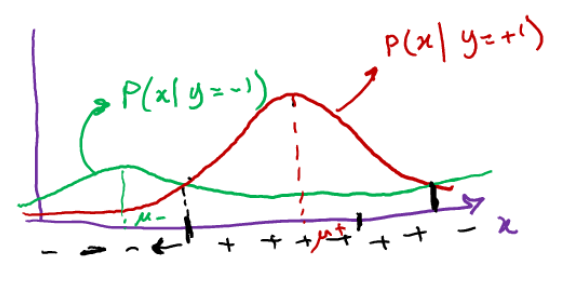
\includegraphics[width=0.5\textwidth]{figures/1d_decision_boundaries.png}
  \caption{Decision boundaries of a 1D scenario of binary NB classifier}
  \label{fig:binary_nb_decision_boundary}
\end{figure}

\end{description}

\subsection{Generative modelling with Bayes}

\begin{itemize}
\item Model class label as generated from categorical variable:
  \begin{equation*}
    P(Y=y) = p_y \quad y\in\mathcal{Y}=\{1,\ldots, c\}
  \end{equation*}
\item Model features as conditionally independent given $Y$.
  \begin{align*}
    P(X_1,\ldots, X_d|Y)&=\prod_{i=1}^{d}P(X_i|Y)\\
    P(X_1=\mathbf{x}_1,\ldots, X_d=\mathbf{x}_d|Y=y)&=\prod_{i=1}^{d}P(X_i=\mathbf{x}_i|Y=y_i)\\
  \end{align*}
Which is equivalent to saying that, given a class label, each feature is generated independently of the other features.

The feature distributions still need to be specified ($P(X_i|Y)$).
\end{itemize}

The model features can also be generated from conditionally independent Gaussians:

\begin{equation*}
  P(x_i|y)=\mathcal{N}(x_i|\mu_{y,i},\sigma^2_{y,i})
\end{equation*}
So the features depend on class $y$ and feature $i\in\{1,\ldots, d\}$

To estimate these parameters, we use MLE for $P(y)$. We assume that $\mathcal{Y}=\{-1,+1\}$. We want $P(Y=+1)=p$ and $P(Y=-1)=1-p$, and we have $\mathcal{D}=\{(\mathbf{x}_1,y_1), \ldots, (\mathbf{x}_n,y_n)\}$.

We can use $\mathcal{D}$ to estimate $p$ via MLE:
\begin{align*}
  \max_{p'}P(\mathcal{D}|p')&=\prod_{i=1}^{n}p'^{[y_i=1]}(1-p)^{[y_i=0]}\\
                            &=p'^{n_+}(1-p')^{n_-}\quad\text{where }
                    \begin{cases}
                      n_+ \quad\text{number of positive cases in }\mathcal{D}\\
                      n_- \quad\text{number of negative cases in }\mathcal{D}\\
                    \end{cases}
                            &=\max_{p' }\ell(p')
\end{align*}

where
\begin{equation*}
  \ell(p')=n_+\log p'+n_-\log (1-p')
\end{equation*}
and
\begin{equation*}
  {\partial\ell\over\partial p} ={n_+\over p'}+{n_-\over 1-p'}=0\Leftrightarrow p'={n_+\over n_++n_-}
\end{equation*}

Now, when devising decision rules for binary classification, we want to know:
\begin{equation*}
  y=\arg\max_{\hat
    {y'}} P(y'| \mathbf{x})
\end{equation*}
For binary tasks ($c=2$), this is equivalent to:
\begin{equation*}
    y=\text{sign}(\log{P(Y=1|\mathbf{x})\over P(Y=-1|\mathbf{x})})
\end{equation*}
The function $f(\mathbf{x})=\log{P(Y=1|\mathbf{x})\over P(Y=-1|\mathbf{x})}$ is called the discriminant function.

In case of GNB and $c=2$ with constant variance, we have:
\begin{equation*}
  f(\mathbf{x})=\mathbf{w}^T\mathbf{x}+w_0
\end{equation*}
where:
\begin{align*}
  w_0&=log{\hat{p}_+\over1-\hat{p}_+}+\sum_{i=1}^{d}{\hat{\mu}^2_{-,i}-\hat{\mu}^2_{+,i}\over 2\hat{\sigma}^2_{i}}\\
  w_i&={\hat{\mu}_{+,i}-\hat{\mu}_{-,i} \over\hat{\sigma}^2_{-,i}}
\end{align*}

There is a difference between the discriminant function vs. the class probability. Let us define

\begin{align*}
  P(Y=+1|\mathbf{x})&\coloneqq p(x)\\
                    &\Rightarrow f(\mathbf{x})=\log{P(\mathbf{x})\over 1-p(\mathbf{x})}\\
                    &\Rightarrow exp(f(\mathbf{x}))={p(\mathbf{x})\over 1-p(\mathbf{x})}\\
                    &\Rightarrow p(\mathbf{x})={\exp(f(\mathbf{x}))\over 1+\exp(f\mathbf{x})}={1\over1+\exp(-f(\mathbf{x}))}=\sigma(f(\mathbf{x}))
\end{align*}

The same function holds for GNB and logistic regression provided assumptions are not violated; GMG and Log Reg will yield the same prediction.

A significant issue with Naive Bayes model is the conditional independence assumption, which means that features are generated independently given a class label. If there is conditional correlation between class labels, then this assumption is violated. Due to this phenomenon, predictions can become overconfident. This might be fine if we care about the most likely class only, but not if we want to use probabilities for making decision, e.g. with asymmetric losses, etc.

A more general solution is the Gaussian Bayes classifier. Model class label are generated from a categorical variable. Model features are generated by a multivariate Gaussian:
\begin{equation*}
  P(\mathbf{x}|y)=\mathcal{N}(\mathbf{x};\mu_y,\sum_y)
\end{equation*}
In GNB we assumed the covariance matrix $\sum_y$ to equate
\begin{equation*}
  \sum_y =
  \begin{pmatrix}
    \sigma_{y,1}^2 & \ldots & 0 \\
    \vdots & \ddots & \ldots \\
    0 & \ldots & \sigma_{y,d}^2 \\
  \end{pmatrix}.
\end{equation*}

The MLE for the Gaussian Bayes Classifier is, for the class label distribution:

\begin{equation*}
  \hat{p}_y={\text{Count}(Y=y)\over n}
\end{equation*}
and for the features:
\begin{align*}
 \hat{P}(\mathbf{x}|y) &= \mathcal{N}(\mathbf{x};\hat{\mu}_y,\hat{\Sigma}_y)\\
  \hat{\mu}_y &= {1\over \text{Count}(Y=y)}\sum_{i:y_i=y}\mathbf{x}_i\\
  &\hat{\Sigma}_y={1\over \text{Count}(Y=y)}\sum_{i:y_i=y}(\mathbf{x}_i-\hat{\mu}_y)(\mathbf{x}_i-\hat{\mu}_y)^T\\
\end{align*}

The discriminant function for Gaussian Bayesian classifiers is given by:

\begin{equation}\label{eq:discriminantgbc}
  f(\mathbf{x})=\log({p\over 1-p})+{1\over 2}\left[\log{|\hat{\Sigma}_-|\over|\hat{\Sigma}_+|}+((\mathbf{x}-\hat{\mu}_-)^T\Sigma_-^{-1}(\mathbf{x}-\hat{\mu}_-))-((\mathbf{x}-\hat{\mu}_+)^T\Sigma_+^{-1}(\mathbf{x}-\hat{\mu}_+))\right]
\end{equation}

\subsection{Fisher's linear discriminant analysis}

Suppose we fix $p=0.5$. Further, we assume that the covariance matrices are equal. Then equation \ref{eq:discriminantgbc} simplifies to:
\begin{equation*}
  f(\mathbf{x})=\mathbf{x}^T\hat{\Sigma}^{-1}(\hat{\mu}_+-\hat{\mu}_-)+{1\over 2}(\hat{\mu}^T_-\Sigma^{-1}\hat{\mu}_--\hat{\mu}_=^{T}\Sigma^{-1}\hat{\mu}_+)
\end{equation*}
Under these assumptions, we predict
\begin{equation*}
  y = \text{sign}(f(\mathbf{x})) = \text{sign}(\mathbf{w}^T\mathbf{x}+w_0)
\end{equation*}
where
\begin{align*}
  \mathbf{w} &= \hat{\Sigma}^{-1}*(\hat{\mu}_+-\hat{\mu}_-)\\
  w_0 &= {1\over 2} (\hat{\mu}_-^T\Sigma^{-1}\hat{\mu}_- -\hat{\mu}_+^T\Sigma^{-1}\hat{\mu}_+)
\end{align*}

This linear classifier is called the linear discriminant analysis. Provided assumptions are met, LDA will make the same predictions as logistic regression.

An illustration of GNB vs. NB is given in Figure~\ref{fig:gnb_vs_nb}.

\begin{figure}
  \centering
  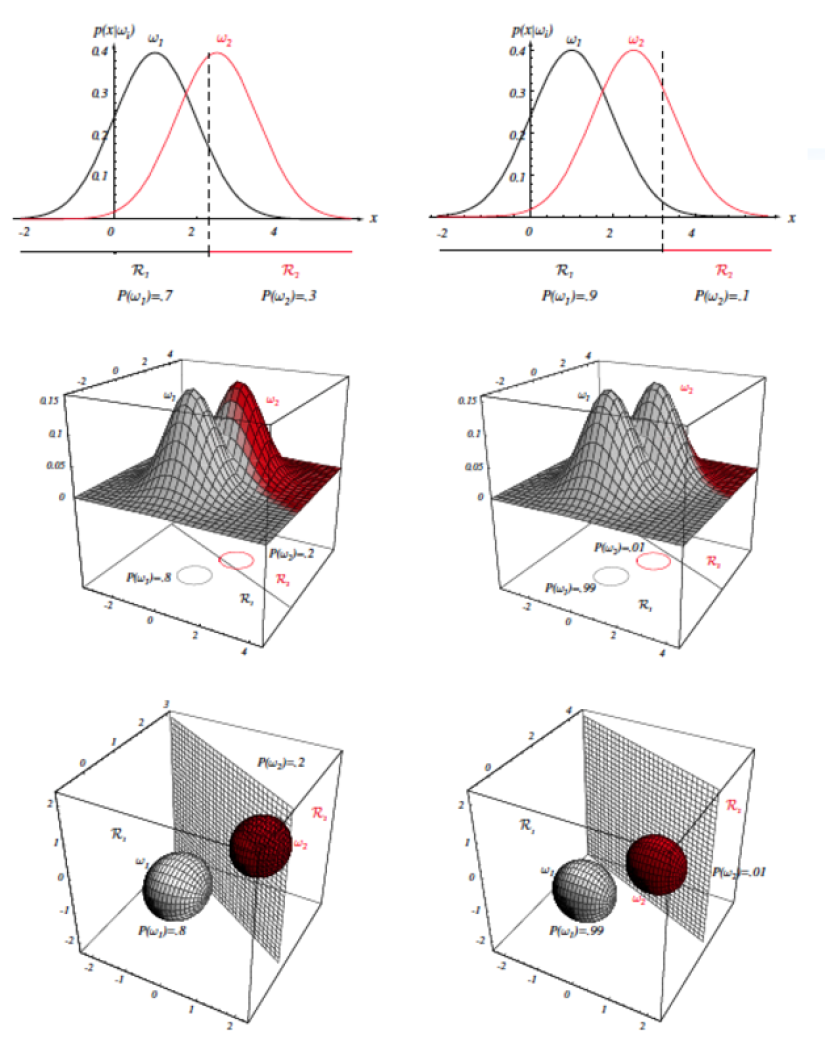
\includegraphics[width=0.5\textwidth]{figures/GNB_vs_NB.png}
  \caption{GNB vs NB}
  \label{fig:gnb_vs_nb}
\end{figure}

Note on LDA vs. PCA. LDA can be viewed as a projection to a 1-dim subspace that maximizes the ratio of between-class and within class variances. In contrast, PCA with $k=1$ maximizes the variance of the resulting 1-dim projection. An illustration is shown in Figure~\ref{fig:lda-vs-pca}.

\begin{figure}
  \centering
  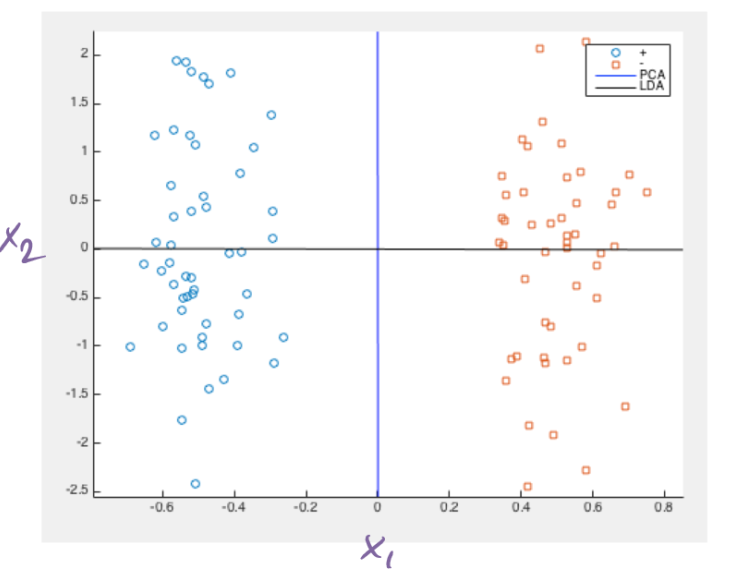
\includegraphics[width=0.5\textwidth]{figures/lda-vs-pca.png}
  \caption{LDA vs. PCA.}
  \label{fig:lda-vs-pca}
\end{figure}

\subsection{Quadratic Discriminant analysis}

In the general case:

\begin{equation*}
  f(\mathbf{x})=\log{p\over 1-p}+{1\over 2}\left[\log{|\hat{\Sigma}_-|\over \hat{\Sigma}_+}\right]+((\mathbf{x}-\hat{\mu}_-)^T\Sigma_-^{-1}(\mathbf{x}-\hat{\mu}_-))-((\mathbf{x}-\hat{\mu}_+)^T\Sigma_+ ^{-1}(\mathbf{x}-\hat{\mu}_ +))
\end{equation*}

We predict $y=\text{sign}f(\mathbf{x})$. This is called quadratic discriminant analysis. This covers a lot more cases, as seen in figure~\ref{fig:qda}. An Euler Diagram showing GBC, LDA, GNB and LR is shown in Figure~\ref{fig:gbclass}.

\begin{figure}
  \centering
  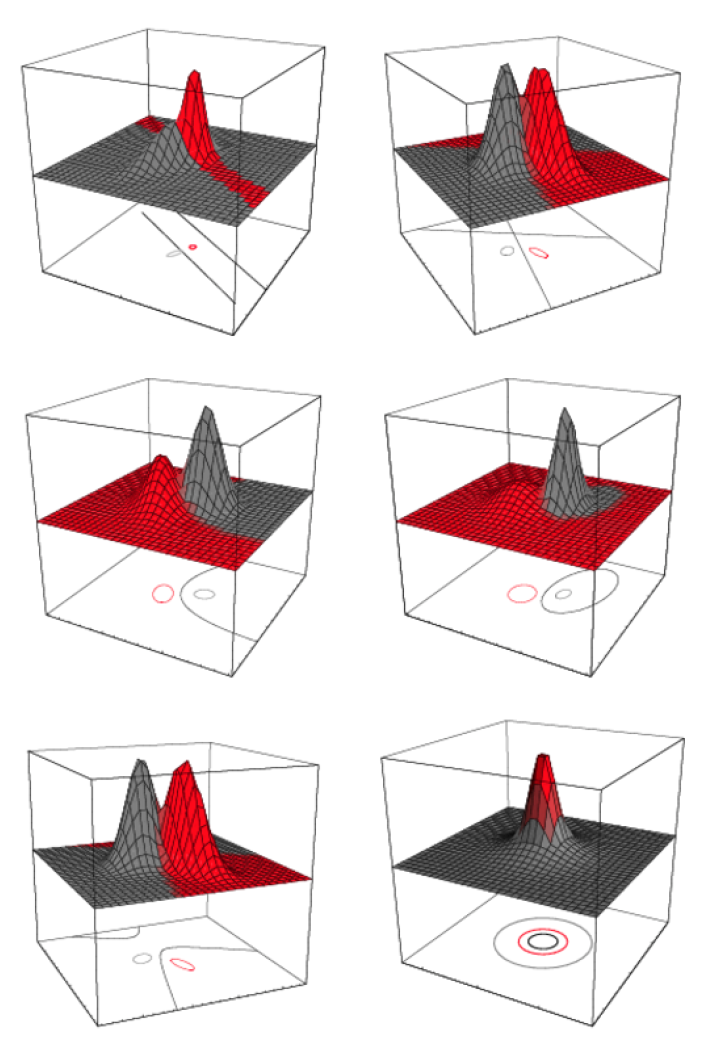
\includegraphics[width=0.4\textwidth]{figures/qda.png}
  \hfill
  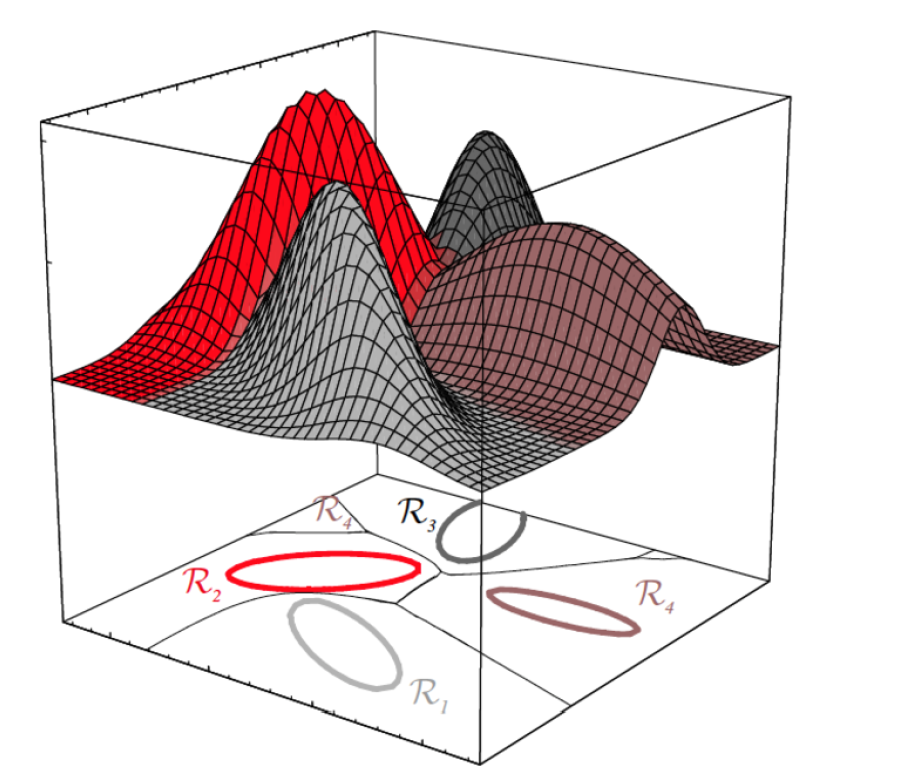
\includegraphics[width=0.4\textwidth]{figures/qda_mutliple_classes.png}
  \caption{Quadratic discriminant analysis illustration }
\label{fig:qda}
\end{figure}

\begin{figure}
  \centering
  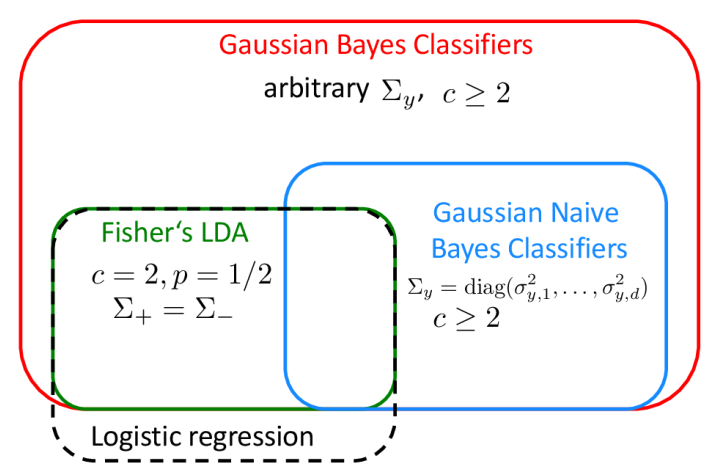
\includegraphics[width=0.5\textwidth]{figures/gbclass.png}
  \caption{Big picture of GB classifiers}
  \label{fig:gbclass}
\end{figure}

Comparing LDA with regression:
\begin{itemize}
\item Fisher's LDA:
  \begin{itemize}
  \item Generative model, i.e., models $P(\mathbf{X},Y)$
  \item Can be used to detect outliers: $P(\mathbf{X})<t$
  \item Assumes normality of $\mathbf{X}$.
  \item Not very robust against violation of this assumption
  \end{itemize}
\item Logistic regression
  \begin{itemize}
  \item Discriminative model, i.e. models $P(\mathbf{X}|Y)$
  \item Cannot detect outliers
  \item Makes no assumptions on $\mathbf{X}$
  \item More robust
  \end{itemize}
\end{itemize}

Comparing GNB vs. more general GBCs:
\begin{itemize}
\item GNB models:
  \begin{itemize}
  \item Conditional independence assumption may lead to overconfidence
  \item Predictions might still be useful
  \item Number of parameters = $\mathcal{O}(cd)$
  \item Complexity (memory + inference) linear in $d$.
  \end{itemize}
\item General Gaussian Bayes models
  \begin{itemize}
  \item Captures correlations among features
  \item avoids overconfidence
  \item number of Parameters = $\mathcal{O}(cd^2)$
    \item Complexity quadratic in $d$.
  \end{itemize}
\end{itemize}

\subsection{Working with categorical features}

If we have discrete features (gender, nationality, ...) it might not make sense to model $X_i$ as Gaussian. Generative models allow to easily swap different distributions, e.g. model $P(X_i|Y)$ as:
\begin{itemize}
\item Bernoulli
\item Categorical
\item Multinomial
\item ...
\end{itemize}
For instance: take a categorical naive Bayes classifier. Model class label as generated from categorical variable, i.e. $P(Y=y)-p_y$ where $y\in\mathcal{Y}=\{1,\ldots,c\}$. Model features are generated by conditionally independent categorical r.v.

\begin{align*}
  P(\mathbf{X}_i=\mathbf{x}|Y=y) &= \theta_{\mathbf{x}|y}^{(i)}\\
  \forall i,\mathbf{x},y:\theta_{\mathbf{x}|y}^{(i)} &\geq 0\\
  \forall i,y:\sum_{i=1}^{c}\theta_{\mathbf{x}|y}^{(i)} &=1\\
\end{align*}

Given dataset $\mathcal{D}=\{(\mathbf{x}_1,y_1),\ldots(\mathbf{x}_n,y_n)\}$. We want and MLE for the class label distribution $\hat{P}(Y=y)=\hat{p}_y$ given by
\begin{equation*}
  \hat{p}_y={\text{Count}(Y=y)\over n}
\end{equation*}
and the MLE for the distribution of feature $i$: $\hat{P}(X_i=c|y)=\theta_{c|y}^{(i)}$
is given by:
\begin{equation}\label{eq:mlefeaturescatnbclass}
  \theta_{c|y}^{(i)}={\text{Count}(X_i=c,Y=y)\over\text{Count}(Y=y)}
\end{equation}

The learning is done as follows:
\begin{itemize}
\item MLE for class prior:
  \begin{equation*}
    \hat{P}(Y=y) = \hat{p}_y={\text{Count}(Y=y)\over n}
  \end{equation*}
  \item MLE for distribution of feature $i$ is given by equation~\ref{eq:mlefeaturescatnbclass}.
\item The prediction given a new point $\mathbf{x}$ is given by:
  \begin{align*}
    y = \arg\max_{y'}\hat{P}(y'|\mathbf{x})&=\arg\max_{y'}\hat{P}(y')\prod_{i=1}^{d}\overbrace{\hat{P}(x_i|y')}^{\text{Categorical}}\\
    &=\arg\max_{y'}\log\hat{p}_y+\sum_{i=1}^{d}\log\theta_{x_i|y'}^{(i)}
  \end{align*}
\end{itemize}

\subsection{Beyond categorical Naive Bayes}

We could in principle lift the NB assumption by modelling a joint conditional distribution of the features: $P(\mathbf{X}_1,\ldots,\mathbf{X}_d|Y)$. The issue here is that the probability of each assignment needs to be specified. It therefore requires exponentially many parameters in $d$, which is computational intractable and overfits. A good remedy is to use graphical models and Bayesian networks.

The Naive Bayes classifier does not require each feature to follow the same type of conditional distribution. For example, this model features that are both Gaussians while other features are categorical. The training (MLE) and prediction remain the same. Given:
\begin{align*}
  X_{1:10}:P(X_i|Y)&=\text{Categorical}(X_i|Y,\theta)\\
  X_{1:10}:P(X_i|Y)&=\mathcal{N}(X_i|\mu_{i,y},\sigma^2_{i,y})\\
\end{align*}
We then have:
\begin{equation*}
  P(X_{1:20}|y)=\prod_{i=1}^{10}\text{Categorical}(X_i|Y,\theta)\prod_{i=11}^{20}\mathcal{N}(X_i|\mu_{i,y},\sigma^2_{i,y})
\end{equation*}

MLE is generally prone to overfitting. This is avoidable by restricting the model class (e.g. assumptions on covariance structure in GNB) which aim to reduce parameters. Using priors can also help.

As prior for our class probabilities in the case that $c=2$, we have $P(Y=1)=\theta$. The MLE is $\hat{\theta}={\text{Count}(Y=1)\over n}$. In the case that $n=1$, we end up with $\hat{\theta}={1\over 1} =1$. We therefore may want to put a prior distribution $P(\theta)$ and compute the posterior distribution using the available data.

\begin{equation*}
  P(\theta|y_1,\ldots,y_n)={1\over z}P(\theta)\cdot P(y_{1:n}|\theta)
\end{equation*}
where $x=\int P(\theta)p(y_{1:n}|\theta)d\theta$.

A natural choice for providing a prior of a r.v. is the beta distribution given by:

\begin{equation*}
  \mathrm {B} (\theta;\alpha_+,\alpha_-)={1\over\mathrm{B}(\alpha_+,\alpha_-)}\theta^{\alpha_+-1}(1-\theta)^{\alpha_--1}
\end{equation*}
Shapes of the p.d.f. of this distribution is shown in Figure~\ref{fig:beta_dist}

\begin{figure}
  \centering
  \includegraphics[width=0.7\textwidth]{figures/beta_distribution.png}
  \caption{Beta distribution under different values of $\alpha_+$ and $\alpha_-$}
  \label{fig:beta_dist}
\end{figure}

Assume observation data $D$ with $n_+$ times $Y=+1$ and $n_-$ times $Y=-1$, then we have:

\begin{equation*}
  p(\theta|D)={1\over z}p(\theta)p(D|\theta)={1\over z'}\theta^{\alpha_+-1}(1-\theta)^{\alpha_--1}\theta^{n_+}(1-\theta)^{n_-}
\end{equation*}

\subsection{Conjugate prior and distributions}

A pair of prior distributions and likelihood functions is called conjugate if the posterior distribution remains in the same family as the prior. For instance, if we take a prior $\mathrm {B} (\theta;\alpha_+,\alpha_-)$ and oberve $n_+$ positives and $n_-$ negatives, the posterior is given by $\mathrm {B} (\theta;\alpha_++x_+,\alpha_-+n_-)$. Here $\alpha_+$ and $\alpha_-$ act as pseudo-counts. The MAP estimate is given by:

\begin{equation*}
  \hat{\theta} = \arg\max_{\theta}p(\theta|y_1,\ldots,y_n;\alpha_+,\alpha_-)={\alpha_++n_+-1\over \alpha_++n_++\alpha_-+n_--2}
\end{equation*}

\begin{table}
  \centering
  \begin{tabular}{ll}
    \toprule
    \textbf{Prior/posterior} & \textbf{Likelihood function}\\
    \midrule
    Beta & Bernouilli/Binomial\\
    Dirichtlet & Categorial/Multinomial\\
    Gaussian (fixed variance) & Gaussian\\
    Gaussian-inverse Wishart & Gaussian\\
    Gaussian process & Gaussian\\
    \bottomrule
  \end{tabular}
  \caption{Conjugate prior and likelihood function}
  \label{tab:likelihood_function}
\end{table}

It is possible to use conjugates as regularizers and add no substantial computational cost. The hyperparameters of these conjugate priors can be chosen using cross validation.

\subsection{Generative vs. Discriminative models}

\begin{itemize}
\item Discriminative models:
  \begin{itemize}
  \item Model $P(y|\mathbf{x})$. Does not attempt to model $P(\mathbf{x})$
  \item Cannot detect outliers (property of $P(\mathbf{x})$
  \item Are typically more robust, since accurately modelling $\mathbf{x}$ may be difficult.
\end{itemize}
\item Generative models
  \begin{itemize}
  \item Model joint distribution $P(\mathbf{x},y)$, which is more ambitious
  \item Can be more powerful if model assumptions are met (can detect outliers)
  \item Are typically less robust against outliers.
  \end{itemize}
\end{itemize}

\subsection{Dealing with missing data}

Missing data can either contain missing labels or missing features. An example of trying to infer class labels from feature distributions is shown in Figure~\ref{fig:gaussian_missing_data}.

\begin{figure}
  \centering
  \includegraphics[width=0.5\textwidth]{figures/Gaussian_Mixtures.png}
G \caption{Gaussian Mixture allows to recover class labels from feature distribution.}
  \label{fig:gaussian_missing_data}
\end{figure}

Figure~\ref{fig:gaussian_missing_data} is provided by a convex combination of Gaussian distributions:
\begin{equation*}
  P(\mathbf{x}|\theta) = P(\mathbf{x}|\mu,\Sigma,\mathbf{w}) = \sum_{i=1}^{c}w_i\mathcal{N}(\mathbf{x}\mu_i,\Sigma_i)
\end{equation*}
where $w_i\geq 0$ and $\sum_iw_i=1$.

\begin{figure}
  \centering
  \includegraphics[width=0.5\textwidth]{figures/Gaussian_mixtures_2.png}
  \caption{Gaussian mixuture, contour and scatterplot}
  \label{fig:gmm2}
\end{figure}

Fitting a mixture model means finding:
\begin{equation*}
  (\mu^*,\Sigma^*,w^*) = \arg\min-\sum_i\log\sum_{j=1}^{k}w_j\mathcal{N}(\mathbf{x}_i|\mu_j\Sigma_j)
\end{equation*}

The MLE for Gaussian mixture is found by minimizing:

\begin{equation*}
  L(w_{1:k},\mu_{1:k},\Sigma_{1:k})=-\sum_{i=1}^{n}\log\sum_{j=1}^{k}w_j\mathcal{N}(\mathbf{x}_i|\mu_j,\Sigma_j)
\end{equation*}

which is non-convex objective.

It is still possible to apply stochastic gradient descent. However, several challenges remain:
\begin{itemize}
\item Covariance matrices must remain symmetric positive definite
\item These constraints might be difficult to maintain.
\end{itemize}

Both GBC and GBB work with the joint distribution. The difference between GBCs in GMMs is that GMMs, the variable $z$ is unobserved. Therefore, fitting a GMM is equivalent to training a GBC without labels. This is equivalent to clustering, because we want to model a latent variable. If we could get the labels, we could compute the MLE in closed form.

Enter: the Hard-EM algorithm. It consists of the following steps:


\begin{itemize}
\item Initialize the parameters $\theta^{(0)}$
\item For $t=1,2,\ldots$:
  \begin{itemize}
  \item \textbf{E-step}: predict the most likely class for each data point:
    \begin{align*}
      z_i^{(t)}&=\arg\max_{z}P(z|\mathbf{x}_i,\theta^{(t-1)})\\
      &= \arg\max_{z}\underbrace{P(z|\theta^{t-1})}_{w_z^{(t-1)}} \underbrace{P(\mathbf{x}_i|z,\theta^{(t-1)})}_{\mathcal{N}(\mathbf{x}_i|\mu_z^{(t-1)},\Sigma_z^{t-1})}
    \end{align*}
  \item The result is complete data.
  \item \textbf{M-step}: compute the MLE as for the GBC, using:
    \begin{equation*}
      \theta^{(t)}=\arg\max_{\theta}P(D^{(t)}|\theta)
    \end{equation*}
  \end{itemize}
\end{itemize}

The problems with the EM algorithm is that points assigned a fixed label, even though the model is uncertain. Intuitively, this tries to extract too much information from a single point. In practice, this may work poorly if clusters are overlapping.

Ideally we want to compute the posterior probabilities of belonging to a cluster. Suppose we're given a model $P(z|\theta)$, $P(\mathbf{x}|z,\theta)$. Then for each data point, we compute a posterior distribution over cluster membership. This means inferring distributions over latent hidden variables $z$ as follows:

\begin{equation*}
  \gamma_j*(\mathbf{x}) = P(Z=j|\mathbf{x},\Sigma,\mu,\mathbf{w}) = {w_j P(\mathbf{x}|\Sigma_j,\mu_j\over \sum_{\ell}w_{ell}P(\mathbf{x}|\Sigma_{ell},\mu_{\ell}))}
\end{equation*}

We can look at this optimality condition as a MLE problem.

\begin{theorem}
  At MLE
  \begin{equation*}
    (\mu^*,\Sigma^*,w^*)=\arg\min-\sum_i\log\sum_{j=1}^kw_j\mathcal{N}(\mathbf{x}_i|\mu_j,\Sigma_j)
  \end{equation*}
  the following must hold:
  \begin{align*}
    \mu_j^*&={\sum_{i=1^n}\gamma_j(\mathbf{x}_i)\mathbf{x}_i\over \sum_{i=1^n}\gamma_j(\mathbf{x}_i)}\\ \Sigma_j^*&={\sum_{i=1}^{n}\gamma_j(\mathbf{x})(\mathbf{x}_i-\mu_j^*)(\mathbf{x}_i-\mu_j^*)^T \over\sum_{i=1}^n\gamma_j(\mathbf{x}_i)}\\
    w_j^*&={1\over n}\sum_{i=1}^{n}\gamma_j(\mathbf{x}_i)
  \end{align*}
\end{theorem}

This allows us to define the soft EM algorithm.

\begin{itemize}
\item While not converged
  \begin{itemize}
  \item \textbf{E-step}: calculate cluster membership weights (aka. expected sufficient statistic or responsibilities) for each point. We calculate $\gamma_j^{(t)}(\mathbf{x}_i)$ for each $i$ and $j $ givenestimates of $\mu^{t-1}$,$\Sigma^{t-1}$,$\mathbf{w}^{(t-1)}$ from the previous iteration.
  \item\textbf{M-step}: fit cluster to weighted data points which corresponds to the maximum likelihood solution:
  \begin{align*}
    w_j^{(t)}&\leftarrow{1\over n}\sum_{i=1}^{n}\gamma_j^{(t)}(\mathbf{x}_i)\\
    \mu_j^{(t)}&\leftarrow{\sum_{i=1}^{n}\gamma_j^{(t)}(\mathbf{x}_i)\mathbf{x}_i\over\sum_{i=1}^{n}\gamma_j^{(t)}(\mathbf{x}_i)}\\
    \Sigma_j^{(t)}&\leftarrow{\sum_{i=1}^n\gamma_j^{(t)}(\mathbf{x}_i)(\mathbf{x}_i-\mu_j^{(t)})(\mathbf{x}_i-\mu_j^{(t)})^T \over\sum_{i=1}^{n}\gamma_j^{(t)}(\mathbf{x}_i)}
  \end{align*}
  \end{itemize}
\end{itemize}

An illustration of the EM algorithm in action is shown in figure~\ref{fig:emalgopics}.

\begin{figure}
  \centering
  \includegraphics[width=.2\textwidth]{figures/EM1.png}
  \includegraphics[width=.2\textwidth]{figures/EM2.png}
  \includegraphics[width=.2\textwidth]{figures/EM3.png}
  \includegraphics[width=.2\textwidth]{figures/EM4.png}
  \caption{EM algorithm illustration}
  \label{fig:emalgopics}
\end{figure}


\begin{figure}
  \centering
  \includegraphics[width=.4\textwidth]{figures/kmeans.png}
  \includegraphics[width=.4\textwidth]{figures/gmm.png}
  \caption{$k$-means vs. GMM}
  \label{fig:gmmvskmeans}
\end{figure}


Note: we can also have constrained GMMs by tying together parameters in MLE:
\begin{itemize}
\item Spherical: $\Sigma_j=\sigma_j^2\cdot I_j$
\item Diagonal: $\Sigma_j=
  \begin{pmatrix}
    \sigma_{j,1}^{2} & \ldots & 0\\
    \vdots & \ddots & \vdots\\
    0 & \ldots & \sigma_{j,1}^{2}
  \end{pmatrix}
  $ (a.k.a. GNB).
\item Tied $\Sigma_1=\ldots=\Sigma_c$
\item Full
\end{itemize}

The EM algorithm estimating using soft assignments to clusters is called soft EM. The intuitive first attempt we discussed first uses hard assignments, and is called hard EM. In general, soft EM will typically result in higher likelihood values. Reason it can deal better with overlapping cluster. The term EM alone typically refers to soft EM.

\begin{theorem}
  Hard EM with uniform weights and spherical covariances is equivalent to $k$-means.
\end{theorem}
For proof, see slide 32 of lecture 23.

Initialization of EM:
\begin{itemize}
\item For weights, we can typically use a uniform distribution
\item For means, we randomly initialize them and k-means++.
\item For variances, we initialize them as spherical, e.g. according to empirical variance in the data.
\end{itemize}

Selecting $k$: in GMMs, we face a similar challenge of selecting the number of clusters. We can generally use the same techniques. However, in contrast to $k$-means, for GMMs typically cross-validation works fairly well. It aims to maximize log-likelihood on the validation set. If the data is truly generated from a GMM, using cross-validation can be used to select $k$. See Figure~\ref{fig:selecting_k_gmm}.

\begin{figure}
  \centering
  \includegraphics[width=.8\textwidth]{figures/selecting_k_gmm.png}
  \caption{Selecting $k$ in GMM.}
  \label{fig:selecting_k_gmm}
\end{figure}

\subsection{Degeneracy of GMMs}

Suppose we are given a single data point. What is the optimal log-likelihood that can be achieved? Well, because
\begin{equation*}
  -\log P(x|\mu,\sigma)={1\over 2}\log(2\pi\sigma^2)+{1\over 2\sigma^2}(x-\mu)^2
\end{equation*}
Small variances will be encouraged and the model won't generalize at all. See Figure~\ref{fig:degeneracy_gmm}. The loss essentially converges to 0 as $\mu=x,\sigma\rightarrow 0$. Thus, an optimal GMM chosses $k=n$, and puts one Gaussian around each data point with variance tending to 0. This is overfitting.

\begin{figure}
  \centering
  \includegraphics[width=.3\textwidth]{figures/degeneracy_gmm_1.png}
  \includegraphics[width=.3\textwidth]{figures/degeneracy_gmm_2.png}
  \caption{Degeneracy of GMM. Red, what happens without regularization, green is what we want: wider variance for better generalization.}
\label{fig:degeneracy_gmm}
\end{figure}

Overfitting can be avoided by adding a small term to the diagonal of the MLE as follows:
\begin{equation*}
  \Sigma_j\leftarrow {\sum_{i=1}^{n}\gamma_j^{(t)}(\mathbf{x})(\mathbf{x}-\mu_i^{(j)})(\mathbf{x}-\mu_i^{(j)})^T\over\sum_{i=1}^{n}\gamma_j^{(t)}(\mathbf{x})}+\mu^2\mathbf{I}
\end{equation*}

This can be motivated from a Bayesian standpoint: this is equivalent to placing a conjugate Wishart prior on the covariance matrix, and computing the MAP instead of the MLE to regularize. $\mu$ can be chosen by cross-validation.

\subsection{Gaussian Mixtures Bayes Classifiers}

GMMs are useful because:
\begin{itemize}
\item Can encode information about shape of clusters.
\item Can be part of more complex statistical models.
 \item Probabilistic models can output the likelihood $P(\mathbf{x})$ of a point $\mathbf{x}$, which is useful for anomaly or outlier detection, and therefore can
   be naturally used for semi-supervised learning.
 \end{itemize}

 A Gaussian Mixture Bayes classifier is defined as follows:

 \begin{itemize}
 \item Given $\mathcal{D} = {(\mathbf{x}_1,y_1),\ldots,(\mathbf{x}_n,y_n)}$, where the label $y\in\{1,\ldots, m\}$, we estimate the class prior $P(y)$ and estimate the conditional distribution for each class:
 \begin{equation*}
   P(\mathbf{x}|y)=\sum_j w_j^{(y)}\mathcal{N}(\mathbf{x};\mu_{j}^{(y)},\Sigma_j^{(y)})
 \end{equation*} as a Gaussian mixture model.
\item To use this model for classification, we perform the following:
  \begin{equation*}
    P(y|\mathbf{x})={1\over Z}p(y)\sum_{j=1}^{k_y}w_j^{(y)}\mathcal{N}(\mathbf{x};\mu_j^{(y)},\Sigma_j^{(y)})
  \end{equation*}
 \end{itemize}

 \begin{figure}
   \centering
   \includegraphics[width=.3\textwidth]{figures/clustering_for_non_linear_classification.png}
   \includegraphics[width=.3\textwidth]{figures/gaussian_mixture_model.png}
   \caption{Clustering for non linear features vs. Gaussian mixture Bayes classifier.}
   \label{fig:power_of_bayes}
 \end{figure}

GMMs can also be used for density estimation. We may be interested in fitting a Gaussian mixture model not for clustering but for density estimation. This combines the advantage of accurate predictions and robustness from discriminative models with the ability to detect outliers.

We can perform anomaly detection with mixture models by comparing the estimated density of the a data point against a threshold, see Figure~\ref{fig:gmm_anomaly_detection}.

\begin{figure}
  \centering
  \includegraphics[width=.5\textwidth]{figures/anomaly_detection_with_mixture_models.png}
  \caption{GMM for anomaly detection.}
  \label{fig:gmm_anomaly_detection}
\end{figure}

Picking the threshold is tricky if we have no examples. If we do have some examples, varying the threshold trades false-positives and false-negatives. One can use PR-curves and ROC curves as evaluation criterion; e.g. maximize the F1 score. the threshold can also be optimized via cross-validation.

GMMs allow one to combine unlabeled and labeled data in a semi supervised learning context. In SSL, for instances $\gamma_j(\mathbf{x}_i)=[j=y_i]$

The EM algorithm for semi-supervised learning with GMM goes as follows:

While not converged:
\begin{itemize}
\item \textbf{E-step}: for unlabeled points:
  \begin{equation*}
    \gamma_j^{(t)}(\mathbf{x}_i)=P(Z=j|\mathbf{x}_i,\mu^{(t-1)},\Sigma^{(t-1)},\mathbf{w}^{(t-1)})
  \end{equation*}
  and for labeled points
  \begin{equation*}
    \gamma_j^{(t)}(\mathbf{x}_i)=[j=y_i]
  \end{equation*}
  \item\textbf{M-step}: Fit clusters to weighted data points, which corresponds to the closed form of the maximum likelihood solution described above, i.e. maximize
  \begin{equation*}
    \theta^{(t)}=\arg\max_{\theta}Q(\theta;\theta^{(t-1)})
  \end{equation*}
\end{itemize}

\subsection{Theory behind the EM algorithm}

We can show that the EM algorithm is equivalent to the following procedure:
\begin{itemize}
\item \textbf{E-step}: calculate the expected complete data log likelihood, which is equivalent to a function of $\theta$:

\begin{align*}
  Q(\theta;\theta^{(t-1)})&=\mathrm{E}_{z_{1:n}}[\log P(\mathbf{x}_{1:n},\mathbf{z}_{1:n}|\theta)|\mathbf{x}_{1:n},\theta^{(t-1)}]\\
                          &=\sum_{z_{1:n}} P(z_{1:n}|\mathbf{x}_{1:n},\theta^{(t-1)})\underbrace{\log P(\mathbf{x}_{1:n},z_{1:n}|\theta^{(t-1)})}_{\text{Complete data log-likelihood}}
\end{align*}
\item \textbf{M-step}: maximize $\theta^{(t)}=\arg\max_{\theta} Q(\theta;\theta^{(t-1)})$
\end{itemize}

Note that the EM objective function can be simplified to:
\begin{equation*}
  Q(\theta;\theta^{(t-1)}) = \sum_{i=1}^{n}\sum_{j=1}^{k}\underbrace{P(z_i=j|\mathbf{x}_i,\theta^{(t-1)})}_{\gamma_j(\mathbf{x}_i))}\log \underbrace{P(\mathbf{x}_i,z_i=j|\theta)}_{w_j\mathcal{N}(\mathbf{x}_i,\mu_j,\Sigma_j)}
\end{equation*}
Thus, the E-step is equivalent to computing $\gamma_z(\mathbf{x}_i)$, which are called expected sufficient statistics. See slide 25 of lecture 24 for the complete derivation.

In the M-step, we need to compute:
  \begin{equation*}
    \theta^{(t)}=\arg\max_{\theta}Q(\theta;\theta^{(t-1)})
  \end{equation*}
  which is very similar to the MLE of the GBC:
    \begin{equation*}
    \theta^{*}=\arg\max_{\theta}\sum_{i-1}^{n}\log P(\mathbf{x},z_i|\theta)
  \end{equation*}
Thus, each iteration of the M-step is equivalent to training a GBC with weighted data and has a closed form solution.

\begin{theorem}\label{th:emconvergence}
  The EM algorithm monotonically increases the likelihood, i.e. the following holds:
  \begin{equation*}
    \log P(\mathbf{x}_{i:n}|\theta^{(t)})\geq \log P(\mathbf{x}_{i:n}|\theta^{(t-1)})
  \end{equation*}
\end{theorem}

For GMMs, EM is guaranteed to converge to a local maximum. The quality of the solution highly depends on the initialization, as in $k$-means. A common strategy is to rerun the algorithm multiple times and use the solution with the largest likelihood. The proof of Theorem \ref{th:emconvergence} is shown in slides 29-31 of slide deck 24 and slides 1-9 of slide deck 25.

The EM algorithm is much more widely applicable. It can be used whenever the E and M steps are tractable, that means we must just be able to compute and maximize the complete data likelihood. Furthermore, this algorithm can be used, for instance, for some missing features, and likelihoods beyond Gaussian (e.g. categorical).

\section{Generative Modelling with Neural Networks}

So far, we have considered very simple probabilistic models (hand selected priors, and likelihood functions). These fail to capture complex, high-dimensional data types like images and audio.

\subsection{Implicit generative models}

Given a sample of unlabeled points $\{\mathbf{x}_1,\ldots,\mathbf{x}_n\}$, the goal is to learn a model $\mathbf{X}=G(\mathbf{Z};\mathbf{w})$ where $\mathbf{Z}$ is a simple distribution (e.g. low dimensional Gaussian). and $G$ some flexible nonlinear function approximated by a neural net. A schemaic mapping of this function is shown in Figure~\ref{fig:implicit_generative_models}:

\begin{figure}
  \centering
  \includegraphics[width=.5\textwidth]{figures/mapping_generative_models.png}
  \caption{Implicit generative models}
  \label{fig:implicit_generative_models}
\end{figure}

The key challenge here is to compute the likelihood of the data. Thus, we need an alternative/surrogate objective functions for training. Variants exist, such as VAE and GANs.

\subsection{Generative Adversarial Networks}

By Goodfellow et al, the goal is to optimize parameters $\mathbf{w}$ to make samples from model hard to distinguish from a data sample. Therefore, one can use a discriminative model to train a generative model. The generator tries to produce realistic examples which the discriminator tries to detect fake examples.

\begin{figure}
  \centering
  \includegraphics[width=.5\textwidth]{figures/GAN_scheme.png}
  \caption{GAN setup}
  \label{fig:gan_setup}
\end{figure}

Formally:

\begin{align*}
  D:\mathrm{R}^d&\rightarrow [0,1]\text{ wants }: D(\mathbf{x}) =
  \begin{cases}
    \approx 1\text{ if }x\text{is real}\\
    \approx 0\text{ if }x\text{is fake}
  \end{cases}
  G:\mathrm{R}^m&\rightarrow \mathrm{R}^d\text{ wants }: D(G(\mathbf{z})) \approx 1\text{ for samples} z
\end{align*}
The overall training objective is:
\begin{equation*}
  \min_G\max_D\underbrace{\mathrm{E}_{\mathbf{X}\sim\mathcal{D}}\log D(\mathbf{x}) +\mathrm{E}_{\mathbf{X}\sim\text{Noise}}\log (1- D(\mathbf{x}))}_{M(G,D)}
\end{equation*}

Training a GAN requires finding a saddle point rather than a local minimimum, due to:
\begin{equation*}
  \min_{\mathbf{w}_G}\max_{\mathbf{w}_D}M(\mathbf{w}_G,\mathbf{w}_D)
\end{equation*}
as illustrated in Figure~\ref{fig:gan_optim_landscape}. Another illustration is shown in Figure to show how the training process approximates the distribution of the data.

\begin{figure}
  \centering
  \includegraphics[width=0.5\textwidth]{figures/GAN_optim_landscape.png}
  \caption{Gan optimization landscape and objective (red dot).}
  \label{fig:gan_optim_landscape}
\end{figure}

\begin{figure}
  \centering
  \includegraphics[width=.8\textwidth]{figures/GAN_training_process.png}
  \caption{GAN training process, the number of iterations increases from left to right}
  \label{fig:gan_iterations}
\end{figure}

GANs have a convergence guarantee. If $G$ and $D$ have enough capacity, then the data generating distribution is indeed the saddle point of:
\begin{equation*}
  \min_{\mathbf{w}_G}\max_{\mathbf{w}_D}M(\mathbf{w}_G,\mathbf{w}_D)
\end{equation*}

Key idea: the best possible discriminator $\ell^*=\max_{\mathbf{w_D}}M(\mathbf{w}_G,\mathbf{w}_D)$ is up to constants the Jensen-Shannon divergence $JS(p_{\text{Data}}||q_{\text{Generator}})$. Where:

\begin{equation*}
  JS(p||q) = {1\over 2}\text{KL}(p||{p+q\over 2})+{1\over 2}\text{KL}(q||{p+q\over 2}); JS(p||q)=0\Leftrightarrow p=q.
\end{equation*}
 In practice, we train a GAN on a finite sample. While we run into the danger of running into the memorization trap, diminishing the power of the discriminator can help alleviate that.

Training approaches for GAN is to simultaneously apply stochastic gradient descent to the empirical GAN objective.

\begin{align*}
  \mathbf{w}_G^{(t+1)} &= \mathbf{w}_G^{(t)} - \eta\nabla_{\mathbf{w}_G}M(\mathbf{w}_G,\mathbf{w}_D^{(t)})\\
  \mathbf{w}_G^{(t+1)} &= \mathbf{w}_G^{(t)} + \eta\nabla_{\mathbf{w}_D}M(\mathbf{w}_G^{(t)},\mathbf{w}_D)\\
\end{align*}

Gradients are approximated by samples of data points.

Note that when training GANs, there is a risk of oscillations and divergence. See Figure~\ref{fig:oscillations_gan_training}.

\begin{figure}
  \centering
  \includegraphics[width=.6\textwidth]{figures/oscillations_gan_training.png}
  \label{fig:oscillations_gan_training}
  \caption{Oscillations: a challenge when training GANs.}
\end{figure}

Another issue that arises is mode collapse, when GANs only model parts of the mode of a distribution. One way to solve this is e.g. in VEEGAN, see Figure~\ref{fig:mode_collapse}.

\begin{figure}
  \centering
  \includegraphics[width=.5\textwidth]{figures/gan_mode_collapse.png}
  \caption{VEEGAN as a solution to mode collapse.}
  \label{fig:mode_collapse}
\end{figure}

When evaluating GANs, it is not possible to compute the likelihood on a holdout set. Generally, it's a difficult problem with no well-accepted and domain independent solution. There are various heuristics though such as the inception score \& FID for images. This remains an open area of research.

\end{document}